\RequirePackage{lineno}
\documentclass[article, a4paper, 11pt, amsmath, amssymb]{revtex4-1}
\usepackage[dvips]{graphicx}
\usepackage{threeparttable}
\usepackage[yyyymmdd,hhmmss]{datetime}


\usepackage{hyperref}
\hypersetup{
    colorlinks=true,
    linkcolor=blue,
    filecolor=magenta,
    urlcolor=cyan,
    pdftitle={Overleaf Example},
    pdfpagemode=FullScreen,
}


% format for abbreviations
\usepackage{enumitem}
\newlist{abbrv}{itemize}{1}
\setlist[abbrv,1]{label=,labelwidth=1in,align=parleft,itemsep=0.1\baselineskip,leftmargin=!}


\usepackage{subfigure}
% \usepackage{subcaption}
\usepackage{indentfirst}
\usepackage{color}
\usepackage{rotating}
\usepackage{footmisc}


% \usepackage{listings}
%\lstset{basicstyle=\footnotesize\ttfamily, breaklines=true, frame=bottomline, escapechar=|}
% styles for code
%\usepackage[charsperline=90]{sty_file/jlcode}
\usepackage{listings}
\usepackage{xcolor}
\definecolor{codegreen}{rgb}{0,0.6,0}
\definecolor{codegray}{rgb}{0.5,0.5,0.5}
\definecolor{codepurple}{rgb}{0.58,0,0.82}
\definecolor{backcolour}{rgb}{0.95,0.95,0.92}
\lstdefinestyle{ylw_style}{
    backgroundcolor=\color{backcolour},
    commentstyle=\color{codegreen},
    keywordstyle=\color{magenta},
    numberstyle=\tiny\color{codegray},
    stringstyle=\color{codepurple},
    basicstyle=\ttfamily\scriptsize\linespread{1.0}\selectfont,
    breakatwhitespace=false,
    breaklines=true,
    captionpos=b,
    keepspaces=true,
    numbers=left,
    numbersep=5pt,
    showspaces=false,
    showstringspaces=false,
    showtabs=false,
    tabsize=4
}
\lstset{style=ylw_style}


\pagestyle{plain}
\bibliographystyle{apsrev}
\DeclareGraphicsExtensions{.eps, .mps, .pdf, .jpg, .png}

\begin{document}
\setpagewiselinenumbers
\modulolinenumbers[5]


% -------------------------------------------------------------------- %

\begin{titlepage}
    \begin{center}
        \vspace*{1cm}

        \Huge
        \textbf{\LARGE{GPU Programming: When, Why and How?}}\\
        \vspace{0.0cm}
        \textbf{\Large{--- --- A Best Practice Guide}}

        \vspace{0.3cm}

        \textrm{\large{AAA~$^{1}$, BBB~$^{2}$, CCC~$^{3}$, DDD~$^{4}$, EEE~$^{5}$}}\\
        \vspace{1.0cm}
        $^1$ 111\\
        $^2$ 222\\
        $^3$ 333\\
        $^4$ 444\\
        $^5$ 555

        \vspace{2.0cm}

        
\includegraphics[height=5cm]{fig_logo_history/eurocc.png}
        %\hspace{0.8cm}
        %
\includegraphics[height=5cm]{fig_logo_history/enccs.png}

    \end{center}
\end{titlepage}


\begin{abstract}
\textbf{\LARGE{Rules to highlight keywords in this paper}}:
\begin{itemize}
    \item The $Italicized$-$text$ is used to highlight variables from code examples, such as the variables $threadIdx.x$, $threadIdx.y$, and $threadIdx.z$ from code examples.
    \item The~\textbf{black bold} font for normal keywords where we want to highlight them, for example,~\textbf{CUDA/oneAPI/MPI/SYCL}.
    \item The~\textbf{\textcolor{red}{red bold}} font for important keywords, directives, build-in kernels, and some statements in programming languages, like \textbf{\textcolor{red}{threadIdx.x/numpy/@vectorize}}.
    \item The~\textbf{\textcolor{brown}{brown bold}} font for directories, names for files, and flags for compilation. Here are several examples.
        \begin{itemize}
            \item \textbf{\textcolor{brown}{-arch=sm\_XY}}
            \item \textbf{\textcolor{brown}{content/examples/cuda-hip}} directory
            \item \textbf{\textcolor{brown}{CUDA.jl}} for NVIDIA GPUs
            \item \textbf{\textcolor{brown}{\$ export MPICH\_GPU\_SUPPORT\_ENABLED=1}}
            \item \textbf{\textcolor{brown}{cuda\_runtime.h}} and~\textbf{\textcolor{brown}{cuda.h}} for CUDA
        \end{itemize}
\end{itemize}
\end{abstract}


\maketitle


% -------------------------------------------------------------------- %
\clearpage
\tableofcontents
%\lstlistoflistings


% -------------------------------------------------------------------- %
\clearpage
\linenumbers


\section{Introduction}


\par
High Performance Computing (HPC) refers to the use of advanced computing technologies to solve complex problems and perform large-scale simulations or calculations at speeds and scales that are beyond the capabilities of typical desktop or server computers~\cite{hpc}.
HPC integrates systems administration (including network and security knowledge) and parallel programming into a multidisciplinary field that combines digital electronics, computer architecture, system software, programming languages, algorithms and computational techniques~\cite{hpc}.


\par
As one of the most important hardware processors, the Central Processing Unit (CPU) is known for its general-purpose and substantial processing power to execute parallel and computationally intensive tasks in HPC.
Besides CPU, the graphics processing unit (GPU) is a specialized hardware accelerator initially designed to accelerate tasks related to graphics rendering and parallel computation, and have recently been evolved to be powerful, general-purpose, and fully programmable processors, ideally suited to tackle massively parallel computing problems due to their many-core architectures~\cite{gpu_wiki}.


\par
GPU Programming involves writing code to harness the computational power of GPUs for specific tasks, including parallel computing, data processing, and scientific simulations.
However, mastering GPU programming techniques requires intensive expertise in parallel programming, memory management, extensive practical experience, and a commitment to continuous learning due to the continuous development of GPU architectures.
Therefore in this Best Practice Guide (BPG), we provide a systematic and comprehensive information for GPU programming allowing developers to leverage the massively parallel architecture of GPUs to accelerate applications in various domains.
It should be noted that this BPG extends the previously developed series of BPGs~\cite{prace-bpg} (these older guides are still relevant as they provide valuable background information about modern accelerators~\cite{modern-accelerators}, modern processors~\cite{modern-processors}, general purpose GPUs~\cite{gpgpu}, $etc.$)., but mainly covers GPU programming issues focusing on a wide range of programming languages, software environments, and APIs, such as~\textbf{directive-based programming models} (Section~\ref{sec:directive-based-programming-models}),~\textbf{non-portable kernel-based programming models} (Section~\ref{sec:non-portable-kernel-based-programming-models}), and~\textbf{portable kernel-based programming models} (Section~\ref{sec:portable-kernel-based-programming-models}).
In addition, representative high-level frameworks and libraries developed for GPU programming, the general procedures for porting code from CPU to GPU and between different GPU framerowks (Section~\ref{sec:porting_code}) are also discussed in this BPG.
At the last section~\ref{sec:stencil_example}, we provide multiple code samples for the two-dimensional heat diffusion problem using the Stencil technique. 

\section{Why GPUs?}


\subsection{Moore’s Law}


\par
Historically, computational demands have been predominantly linked to the Central Processing Unit (CPU), a complex component governing operations across diverse computing platforms, ranging from desktops to laptops and smartphones. The evolution of the modern CPU has been an intricate journey, driven in large part by the exacting standards set by the scientific and High Performance Computing (HPC) sectors. Transistors, the fundamental units of the CPU, dictate the performance of computers, mobile devices, and other contemporary electronic circuits.

\begin{figure}[!h]
\centering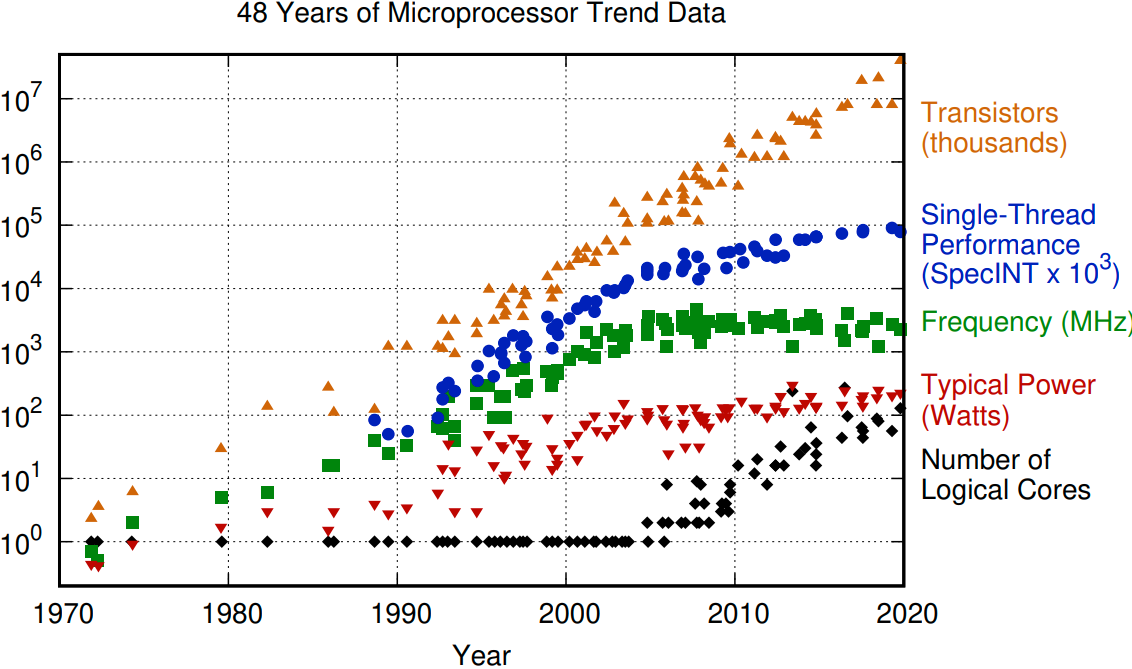
\includegraphics[width=0.8\textwidth]{fig_logo_history/microprocessor_trend.png}
\caption{The Moore’s Law timeline, including Moore's bend with transistors/CPU inflected with multi-core CPUs. Before 2000, the increase in the single core clock frequency was the major source of the increase in the performance. Mid 2000 mark a transition towards multi-core processors. Original data up to the year 2010 collected and plotted by M. Horowitz, F. Labonte, O. Shacham, K. Olukotun, L. Hammond, and C. Batten. New plot and data collected for 2010-2019 by K. Rupp~\cite{microprocessor-trend-data}. }\label{fig:microprocessor_trend}
\end{figure}


\par
\textbf{The Moore's Law} states that the number of transistors in a dense integrated circuit doubles about every two years (Fig.~\ref{fig:microprocessor_trend}).
More transistors means smaller size of a single element, so higher core frequency can be achieved.
Up until the year 2000s, the CPU manufacturers including IBM, Intel, and AMD produce faster CPUs by making them work at a higher speed, 16 MHz, 20 MHz, 66 MHz, 100 MHz, and eventually 200, 333, 466 MHz$\cdots$.
It looks like they could keep increasing the CPU speeds and provide higher performance every year.
However, at the beginning of 2000s, it was obvious that continuously increasing the CPU speeds couldn’t go on forever due to the power consumption limits.
The power consumption scales with frequency to the third power, and therefore the growth in the core frequency has slowed down significantly, which limits the improvement on the computational performance of single-core CPUs.


\par
Increasing computational performance of processing units has been sustained with two main strategies over the years: 1) Increase the single processor performance; and 2) More recently, increase the number of physical cores.
Both strategies promote the development of parallel computing for scientific and HPC community.
In fact, higher performance of a single node has to rely on its more complicated structure and still can be achieved with SIMD (single instruction multiple data), branch prediction, $etc$.


% -------------------------------------------------------------------- %


\subsection{Parallel computing}


\par
Parallel computing, which is interchangeable with parallel processing or in conjunction with parallel programming, refers to the process of decomposing a computational problem into smaller subtasks that can be executed simultaneously using multiple processing units (Fig.~\ref{fig:comput_serial_parallel}).
Parallel computing is critical for large scale projects in which speed and accuracy are needed.
It is a complex task, but allows developers, researchers, and users to accomplish research and analysis quicker than with a program that can only process one task at a time.


\begin{figure}[!h]
\centering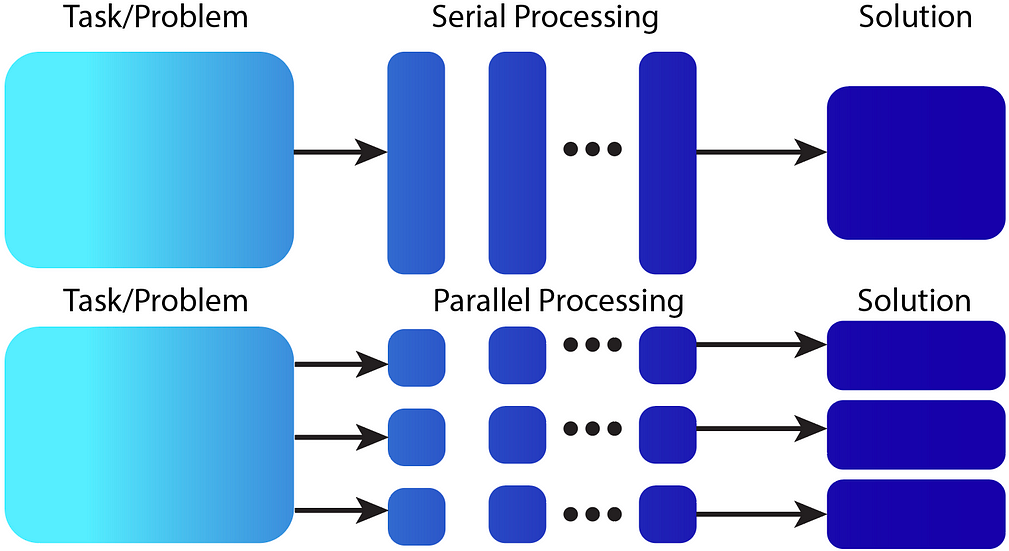
\includegraphics[width=0.8\textwidth]{fig_logo_history/comput_serial_parallel.png}
\caption{Serial processing and parallel computing.}\label{fig:comput_serial_parallel}
\end{figure}


\par
How a problem is split into smaller subtasks strongly depends on the problem.
There are two fundamental types of parallelism in applications:~\textbf{task parallelism} and~\textbf{data parallelism}.
\begin{itemize}
    \item Task parallelism arises when there are many tasks or functions that can be operated independently and largely in parallel. Task parallelism focuses on distributing functions across multiple cores.
    \item Data parallelism arises when there are many data items that can be operated on at the same time. Data parallelism focuses on distributing the data across multiple cores.
\end{itemize}


\par
More pertinently, two of the most commonly used programming approaches are SIMD and MIMD.
SIMD, or single instruction multiple data, is a form of parallel computing related to a computer architecture.
There are multiple cores in the computer.
All cores execute the same instruction stream at any time, each operating on different data streams.
SIMD is typically used to analyze large data sets that are based on the same specified benchmarks.
Vector computers are typically characterized as SIMD, and most modern computers employ a SIMD architecture.
Perhaps the biggest advantage of SIMD is that, while writing code on the CPU, the programmers can continue to think sequentially yet achieve parallel speed-up from parallel data operations because the compiler takes care of the details.
MIMD, or multiple instruction multiple data, is another common form of parallel computing and computer architecture in which multiple cores operate on multiple data streams, each executing independent instructions.
Many MIMD architectures also include SIMD execution sub-components.


\par
Besides SIMD and MIMD, the computer architecture can also be subdivided by its memory organization, which is generally classified into two types:~\textbf{multi-node with distributed memory} and~\textbf{multiprocessor with shared memory}.
In a multi-node system, large scale computational engines are constructed from many processors connected by a network. Each processor has its own local memory, and processors can communicate the contents of their local memory over the network.
The left figure in Fig.~\ref{fig:multinode_vs_multicore} shows a typical multi-node system with distributed memory. These systems are often referred to as~\textbf{clusters}.
Multiprocessor architectures typically range in size from dual-processor to dozens or hundreds of processors. These processors are either physically connected to the same memory (the right figure in Fig.~\ref{fig:multinode_vs_multicore}), or share a low-latency link (such as PCI-Express or PCIe).
Although sharing memory implies a shared address space, it does not necessarily mean there is a single physical memory.
Such multiprocessors include both single-chip systems with multiple cores, known as~\textbf{multicore}, and computers consisting of multiple chips, each of which might have a multicore design.
Multicore architectures have displaced single-core architectures permanently. The term~\textbf{many-core} is usually used to describe multicore architectures with an especially high number of cores (tens or hundreds).
Recently, computer architectures have been transitioning from multicore to many-core, and a representative of many-core computing hardware is graphics processing unit (GPU).


\begin{figure}[!h]
\centering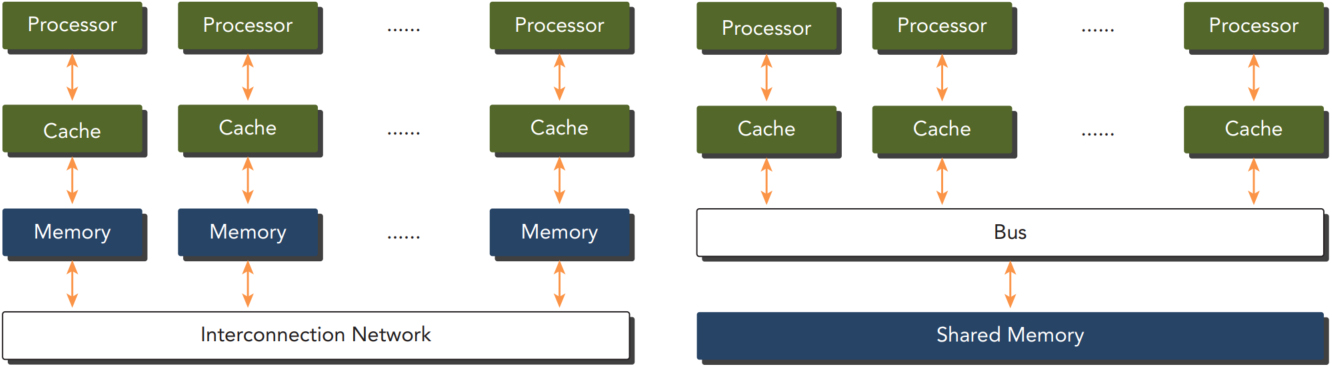
\includegraphics[width=0.9\textwidth]{fig_hardware/multinode_vs_multicore.jpg}
\caption{Two types of computer architectures depending on their memory organization. Left for multi-node with distributed memory and right for multiprocessor with shared memory.}\label{fig:multinode_vs_multicore}
\end{figure}


% -------------------------------------------------------------------- %


\subsection{Graphics processing units}


\par
A GPU is a specialized electronic circuit initially designed to accelerate computer graphics and image processing (either on a video card or embedded on the motherboards, mobile phones, personal computers, workstations, and game consoles), but have recently been evolved to be powerful, general-purpose, fully programmable, task and data parallel processors, ideally suited to tackle massively parallel computing problems due to their many-core architectures~\cite{gpu_wiki}.


% -------------------------------------------------------------------- %


\subsection{Advantages and limitations of CPU and GPU programming}


\par
CPUs have several distinct advantages for modern computing tasks:
\begin{itemize}
    \item Flexibility: a CPU is a general-purpose processor that can handle many tasks, and multitask between multiple activities.
    \item Faster in many contexts: CPUs are faster than GPUs when handling operations like data processing in RAM, I/O operations, and operating system administration.
    \item Precision: CPUs can support mid-range math operations with higher precision than GPUs, which is important for many use cases.
    \item Cache memory: CPUs have a large local cache memory, which lets them handle large sets of linear instructions.
    \item Hardware compatibility: CPUs are compatible with all types of motherboards and system designs, whereas GPUs require specialized hardware support.
\end{itemize}


CPUs have the following disadvantages compared to GPUs:
\begin{itemize}
    \item Parallel processing: CPUs are less adept at tasks that require millions of identical operations because of their limited parallelism.
    \item Slower development: CPUs are a very mature technology that is already reaching the limits of its development, while GPUs have much more potential to improve.
    \item Compatibility: several types of CPUs, including x86 and ARM processors, and software may not be compatible with all types.
\end{itemize}


The unique advantages of GPUs include:
\begin{itemize}
    \item High data throughput: a GPU can perform the same operation on many data points in parallel, so that it can process large data volumes at speeds unmatched by CPUs.
    \item Massive parallelism: a GPU has hundreds of cores, allowing it to perform massively parallel calculations, such as matrix multiplications.
    \item Suitable for specialized use cases: GPUs can provide massive acceleration for specialized tasks like deep learning, big data analytics, genomic sequencing, and more.
    \item Improved energy efficiency: Compared to CPUs, GPUs can perform more calculations per watt of power consumed, which can result in significant energy savings. This is indeed evident from the Green500 list~\cite{green500}.
    \item Cost-effectiveness: GPUs can be more cost-effective than traditional CPU-based systems for certain workloads.
\end{itemize}


The limitations of GPUs compared to CPUs include:
\begin{itemize}
    \item Difficulty handling complexity: Not all workloads can be efficiently parallelized and accelerated on GPUs. A GPU can struggle with processing tasks that are not well structured. They cannot efficiently process branching logic, sequential operations, or other complex programming patterns. % Certain types of workloads, such as those with irregular data access patterns or high branching behavior, may not see significant performance improvements on GPUs.
    \item Steeper learning curve: Depending on the GPU programming API that you choose, GPU computing could require specialized skills in GPU programming and knowledge of GPU architecture, leading to a steeper learning curve compared to CPU programming. Fortunately, if you study this training material closely you will become productive with GPU programming quickly!
\end{itemize}


\par
GPU computing is not meant to replace CPU computing.
Each approach has advantages for certain kinds of programs.
CPU computing is good for control-intensive tasks, and GPU computing is good for data-parallel computation-intensive tasks.
When CPUs are complemented by GPUs, it makes for a powerful combination.
The CPU is optimized for dynamic workloads marked by short sequences of computational operations and unpredictable control flow; and GPUs aim at the other end of the spectrum: workloads that are dominated by computational tasks with simple control flow. 


\par
If a problem has a small data size, sophisticated control logic, and/or low-level parallelism, the CPU is a good choice because of its ability to handle complex logic and instruction-level parallelism.
If the problem at hand instead processes a huge amount of data and exhibits massive data parallelism, the GPU is the right choice because it has a large number of programmable cores, can support massive multi-threading, and has a larger peak bandwidth compared to the CPU.
The CPU + GPU heterogeneous parallel computing architectures evolved as such a combination ensures that the characteristics of the GPU and CPU complement each other, leading to a full utilization of the computational power of the combined CPU + GPU system.


\par
For the heterogeneous architecture, CPUs and GPUs are discrete processing components connected by the PCI-Express bus (Fig.~\ref{fig:cpu_gpu_architecture}).
The switch from traditional homogeneous CPU systems to current heterogeneous CPU+GPU systems is a milestone in the history of HPC.
\textbf{Homogeneous computing} uses one or more processor of the same architecture to execute an application.
\textbf{Heterogeneous computing} instead uses a suite of processor architectures to execute an application, applying tasks to architectures to which they are well-suited, yielding performance improvement as a result.


\begin{figure}[htbp]
\centering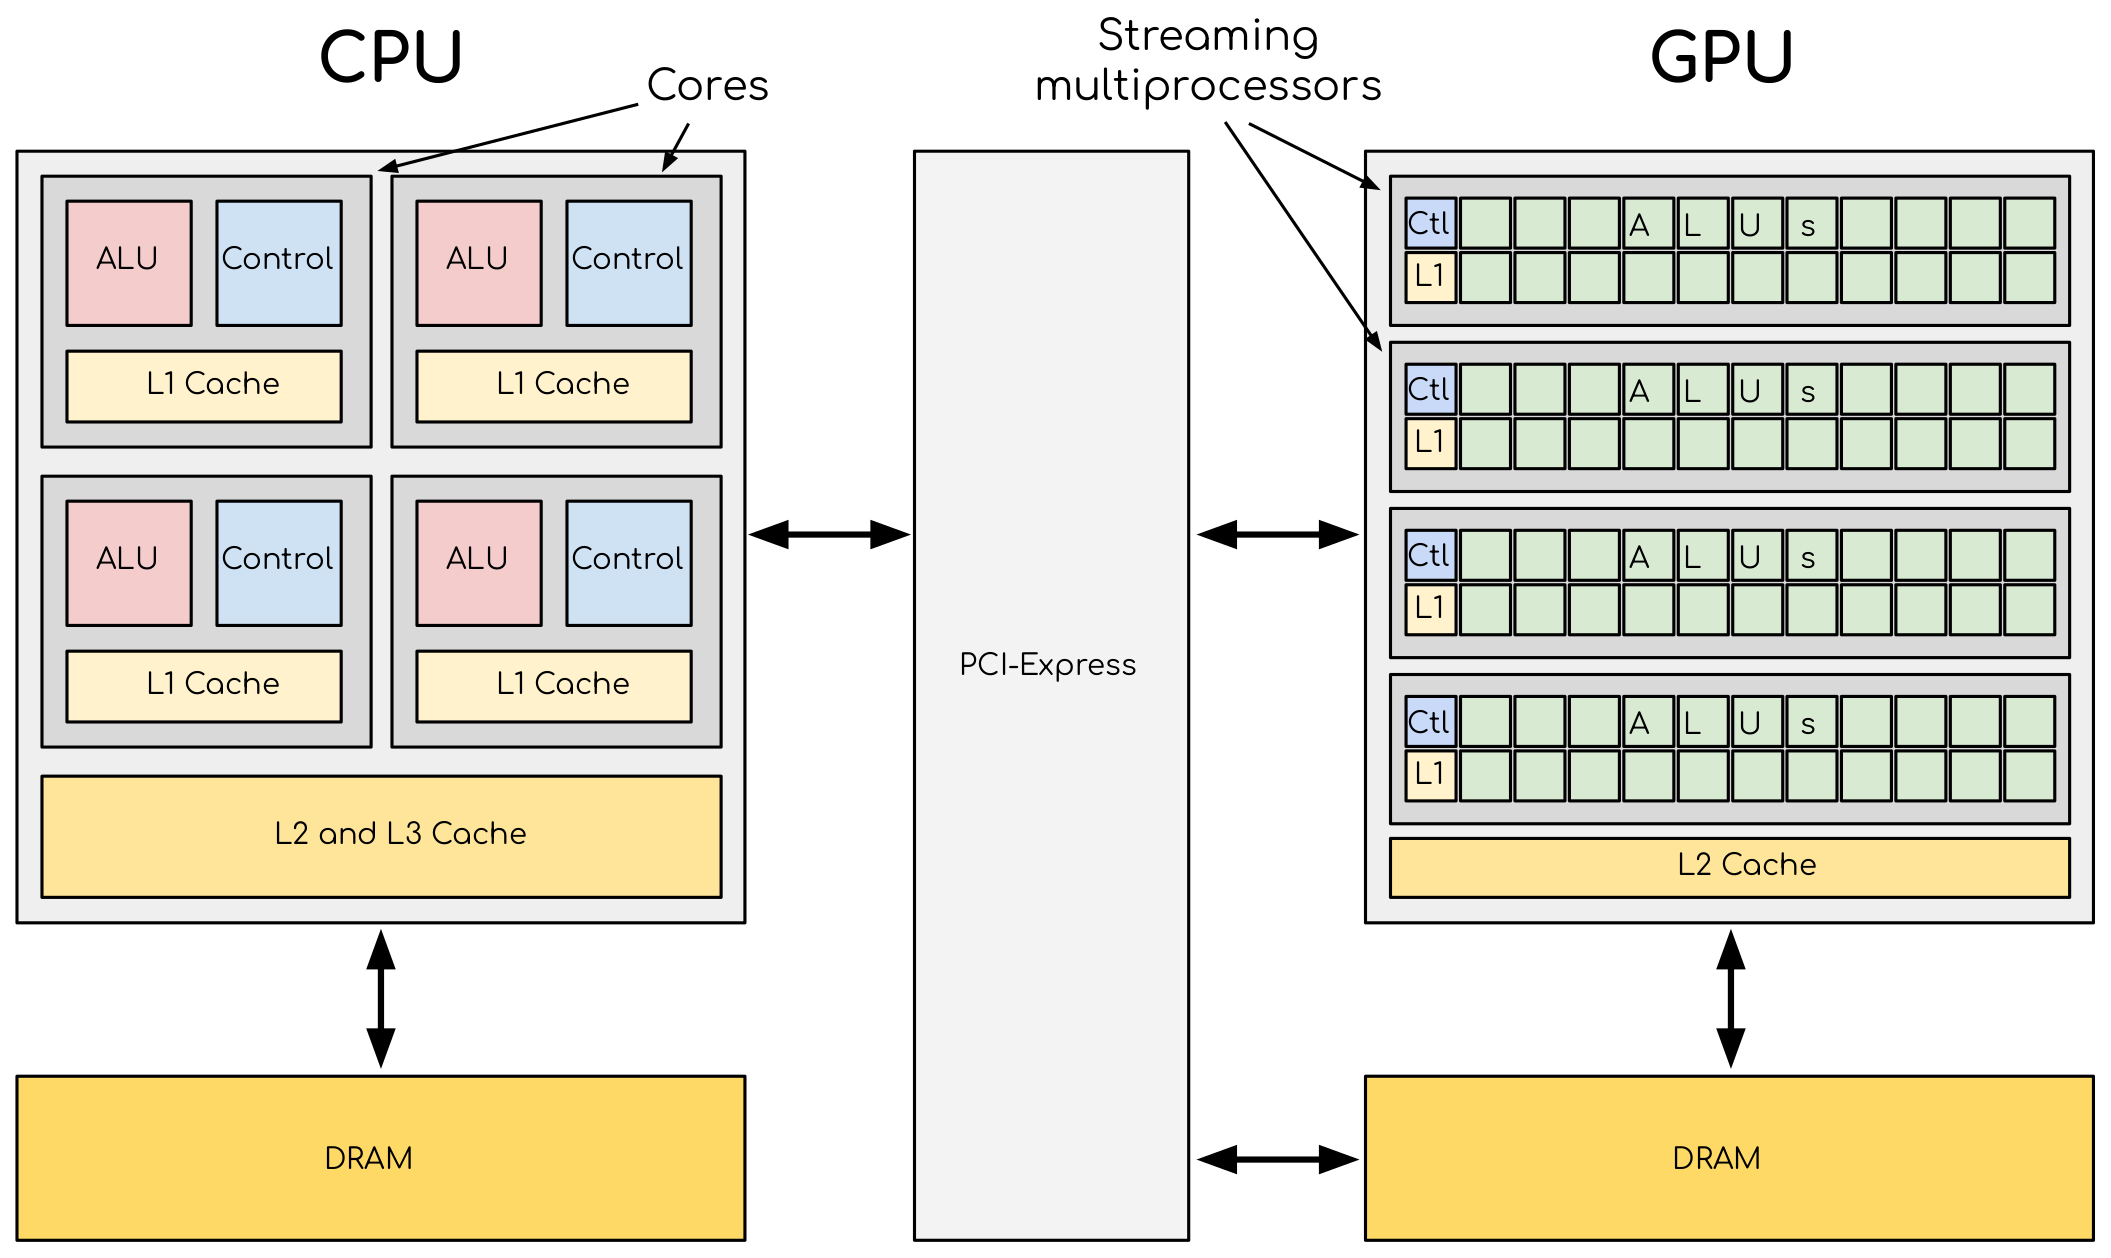
\includegraphics[width=0.8\textwidth]{fig_hardware/cpu_gpu_architecture.png}
\caption{A comparison of CPU and GPU architecture. CPU (left) has complex core structure and pack several cores on a single chip. GPU cores are very simple in comparison, they also share data and control between each other. This allows to pack more cores on a single chip, thus achieving very high compute density.}\label{fig:cpu_gpu_architecture}
\end{figure}


\par
The GPU-enabled heterogeneous computing systems require a heterogeneous programming model that involves both CPU and GPU, where the CPU and its memory are referred to as the~\textbf{host}, and the GPU and its memory as the~\textbf{device}.
Correspondingly, a program running on heterogeneous computing systems consists of two parts, the host code running on CPUs and the device code running on GPUs.
The program executing on a heterogeneous platform is typically initialized by the CPU.
The CPU code is responsible for managing the environment, code, and data for the device before loading compute-intensive tasks on the device.
With computational intensive applications, program sections often exhibit a rich amount of data parallelism. GPUs are used to accelerate the execution of this portion of data parallelism.
Therefore, for optimal performance we need to use both CPU and GPU for computational intensive applications, executing the sequential parts or task parallel parts on the CPU and intensive data parallel parts on the GPU.


\par
To support joint CPU + GPU execution of an application, the three major GPU vendors, NVIDIA, AMD, and Intel, in addition to design and produce GPUs for HPC, have designed their own computing platforms~\textbf{CUDA} (Compute Unified Device Architecture),~\textbf{ROCm} (Radeon Open Compute), and~\textbf{oneAPI}, respectively.
This way they can offer optimization, differentiation (offering unique features tailored to their devices), vendor lock-in, licensing, and royalty fees, which can result in better performance, profitability, and customer loyalty.
There are also cross-platform APIs (application programming interfaces) such~\textbf{DirectCompute} (only for Windows operating system),~\textbf{OpenCL}, and~\textbf{SYCL}.
These are the main topics of this workshop targeted for GPU programming.


% -------------------------------------------------------------------- %


\subsection{The Top500 HPC supercomputers at a glance}


\par
HPC is a set of technologies that enable large-scale, massively parallel computing.
Traditionally, HPC systems were based on CPUs, but modern HPC systems increasingly make use of GPUs.
It is common for HPC servers to combine multiple CPUs and GPUs in one system.


\par
The TOP500 project ranks and details the 500 most powerful non-distributed HPC systems in the world.
This project was launched in 1993 to improve and renew the Mannheim supercomputer statistics, and publishes an updated list of the supercomputers twice a year~\cite{top500_1}.
Fig.~\ref{fig:supercomputer_top5} shows the top-5 HPC systems as of June 2023~\cite{top500_2}, where the columns show:
\begin{itemize}
    \item Cores: Number of processors
    \item Rmax: Maximal LINPACK performance achieved
    \item Rpeak: Theoretical peak performance
    \item Power: Power consumption
\end{itemize}


\begin{figure}[htbp]
\centering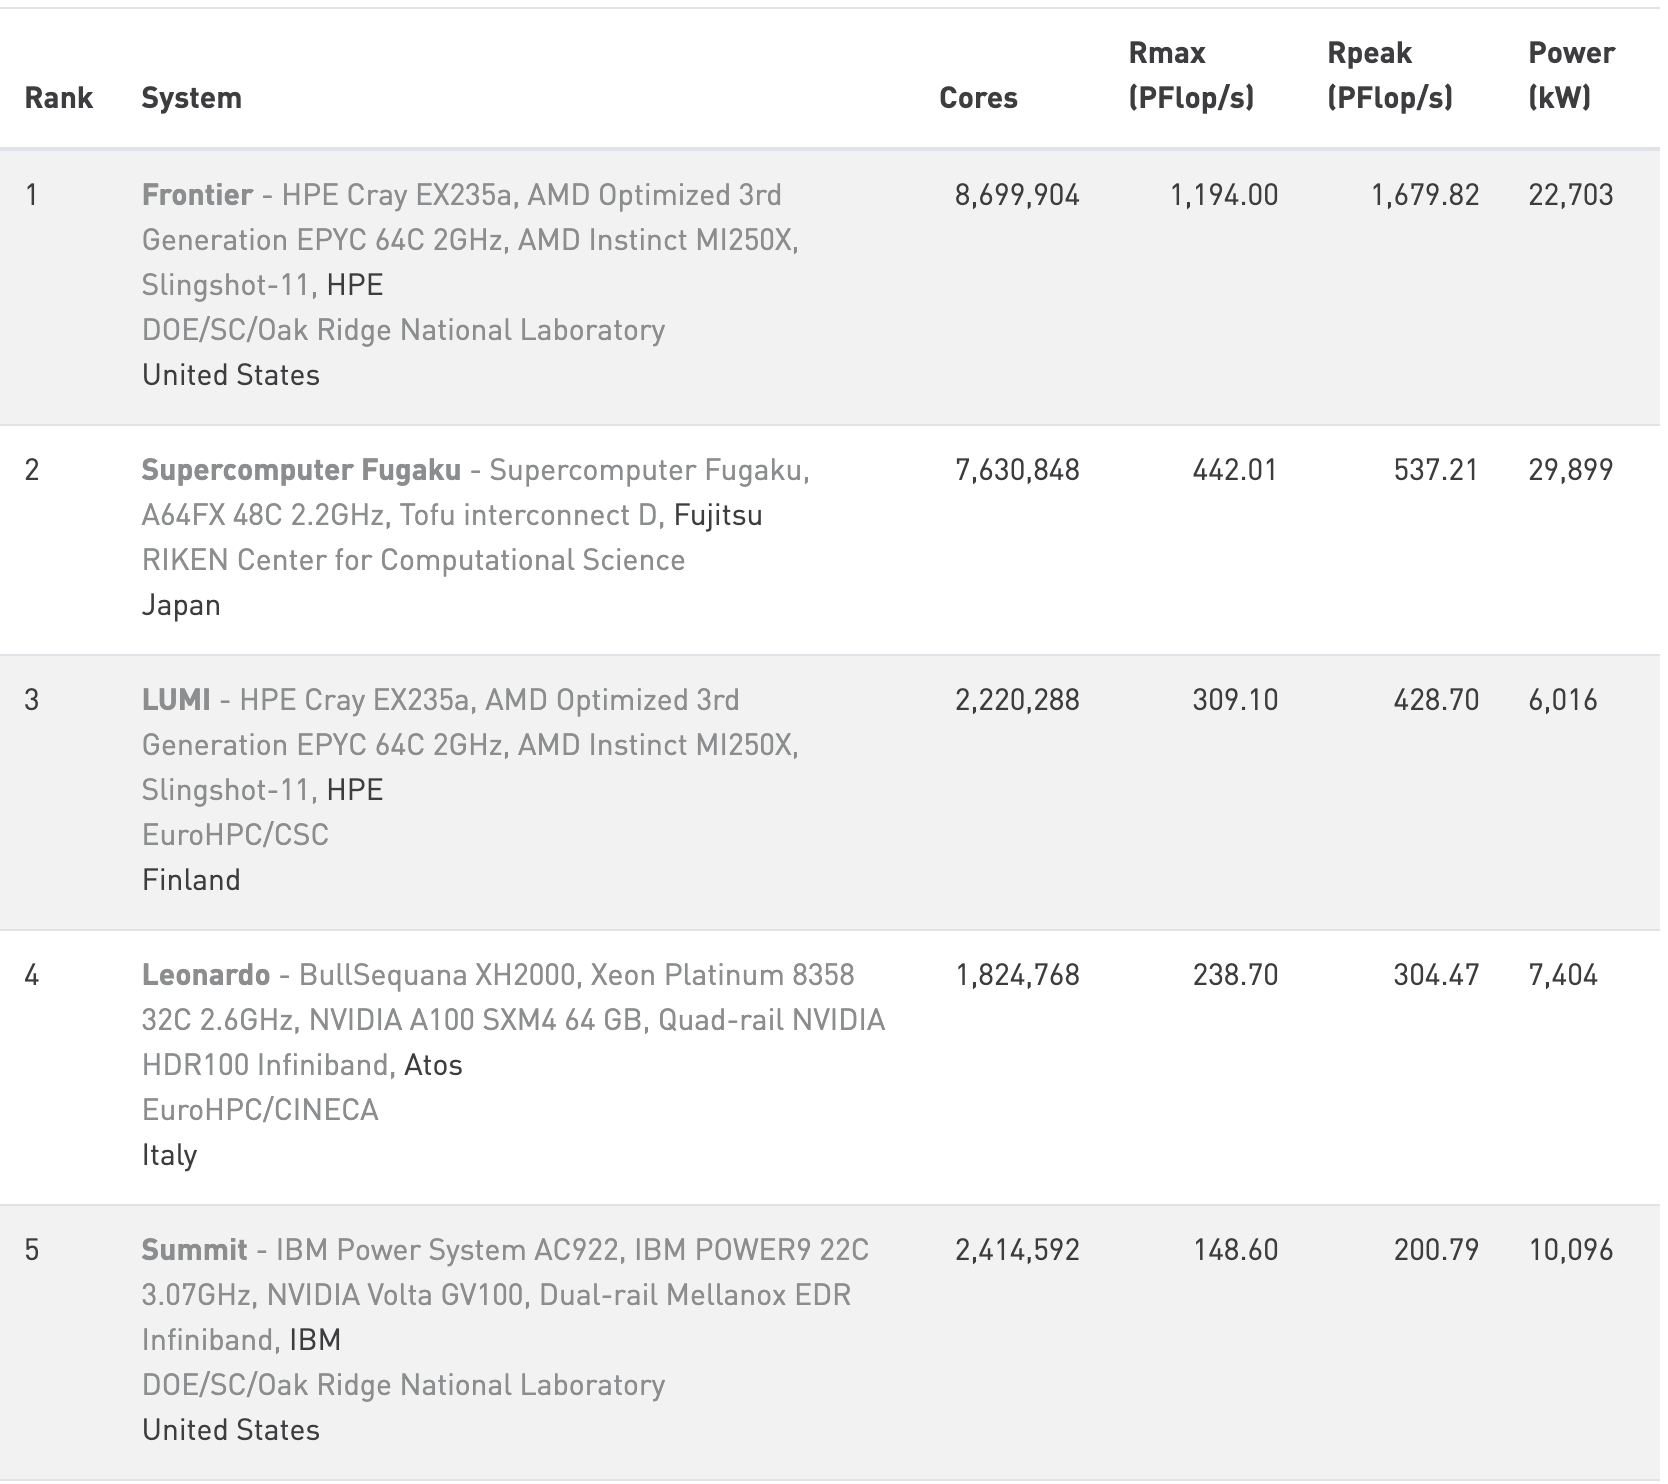
\includegraphics[width=0.8\textwidth]{fig_logo_history/supercomputer_top5.png}
\caption{The top 5 HPC systems on the Top500 list from June, 2023.}\label{fig:supercomputer_top5}
\end{figure}


\par
All systems in the top-5 positions contain GPUs from AMD or NVIDIA, except for the Fugaku system at the RIKEN Center for Computational Science in Kobe, Japan, which instead relies on custom-built Arm A64FX CPUs.
The Frontier system at the Oak Ridge National Laboratory, Tennessee, USA remains the No. 1 system on the TOP500 and is still the only system reported with an HPL performance exceeding one Exaflop/s.
Frontier is based on the latest HPE Cray EX235a architecture and equipped with AMD EPYC 64C 2GHz processors. The system has 8,699,904 total cores, a power efficiency rating of 52.59 gigaflops/watt, and relies on Slingshot-11 interconnect for data transfer.  
The No. 3 and No. 4 HPC systems are the LUMI system at EuroHPC/CSC in Finland and the Leonardo system at EuroHPC/CINECA in Italy, and have HPL scores of 309.1 Pflop/s and 239 Pflop/s, respectively.
The Summit system, also at the Oak Ridge National Laboratory, Tennessee, USA, was launched in 2018 and has a hybrid architecture with each node containing multiple IBM POWER9 CPUs and NVIDIA Volta GPUs all connected together with NVIDIA’s high-speed NVLink.
Each node has over half a terabyte of coherent memory (high bandwidth memory + DDR4) addressable by all CPUs and GPUs plus 800GB of non-volatile RAM that can be used as a burst buffer or as extended memory.


\section{GPU Hardware and Software Ecosystem}


\subsection{Overview of GPU hardware}


\par
GPU hardware is a specialized type of processor designed primarily for rendering and manipulating graphics.
Over times, GPUs have evolved to become highly parallel accelerators capable of performing a wide range of general-purpose computing tasks.
One of the most important features that allows these accelerators to reach their high performance computing capability is their scalability. 
Computational cores on accelerators are usually grouped into multiprocessors, and these multiprocessors share the data and logical elements.
This allows to achieve a very high density of compute elements on a GPU, and also allows for better scaling: more multiprocessors means more raw performance and this is very easy to achieve with more transistors available.


\par
Accelerators are a separate main circuit board with the processor, memory, power management, $etc$.
It is connected to the motherboard with CPUs via PCIe bus(Fig.~\ref{fig:cpu_gpu_architecture}).
Having its own memory means that the data has to be copied to and from it.
CPU acts as a main processor, controlling the execution workflow.
It copies the data from its own memory to the GPU memory, executes the program and copies the results back.
GPUs are coprocessors (helpers) to CPUs, and run tens of thousands of threads simultaneously on thousands of cores and does not do much of the data management.
With many cores trying to access the memory simultaneously and with little cache available, the accelerator can run out of memory very quickly.
This makes the data management and its access pattern is essential on the GPU.
Accelerators like to be overloaded with the number of threads, because they can switch between threads very quickly.
This allows to hide the memory operations: while some threads wait, others can compute.


% -------------------------------------------------------------------- %


\subsection{How do GPUs differ from CPUs?}


\par
CPUs and GPUs were designed with different goals in mind.
While the CPU is designed to excel at executing a sequence of operations, called a thread, as fast as possible and can execute a few tens of these threads in parallel, the GPU is designed to excel at executing many thousands of them in parallel.
GPUs were initially developed for highly-parallel task of graphic processing and therefore designed such that more transistors are devoted to data processing rather than data caching and flow control.
More transistors dedicated to data processing is beneficial for highly parallel computations; the GPU can hide memory access latencies with computation, instead of relying on large data caches and complex flow control to avoid long memory access latencies, both of which are expensive in terms of transistors.
A short summary of the difference between CPU and GPU is provided in Table~\ref{tbl:difference_cpu_gpu}.


\begin{table}[!h]
\centering\caption{The general difference between CPU and GPU.}\label{tbl:difference_cpu_gpu}
\begin{tabular}{ |c|c| }
\hline
\textbf{CPU} & \textbf{GPU} \\
\hline
General purpose & Highly specialized for parallelism \\ 
Good for serial processing & Good for parallel processing \\ 
Great for task parallelism & Great for data parallelism \\ 
Low latency per thread & High-throughput \\
Large area dedicated cache and control & Hundreds of floating-point execution units \\
\hline
\end{tabular}
\end{table}


% -------------------------------------------------------------------- %


\subsection{GPU platforms}


\par
GPUs come together with software stacks or APIs that work in conjunction with the hardware and give a standard way for the software to interact with the GPU hardware.
They are used by software developers to write code that can take advantage of the parallel processing power of the GPU, and they provide a standard way for software to interact with the GPU hardware.
Typically, they provide access to low-level functionality, such as memory management, data transfer between the CPU and the GPU, and the scheduling and execution of parallel processing tasks on the GPU.
They may also provide higher level functions and libraries optimized for specific HPC workloads, like linear algebra or fast Fourier transforms. 
Finally, in order to facilitate the developers to optimize and write correct codes, debugging and profiling tools are also included.


\par
Three major GPU vendors, NVIDIA, AMD, and Intel, have designed their own computing platforms~\textbf{CUDA},~\textbf{ROCm}, and~\textbf{oneAPI}, respectively.
This way they can offer optimization, differentiation (offering unique features tailored to their devices), vendor lock-in, licensing, and royalty fees, which can result in better performance, profitability, and customer loyalty.
There are also cross-platform APIs such~\textbf{DirectCompute} (only for Windows operating system),~\textbf{OpenCL}, and~\textbf{SYCL}.


\subsubsection{CUDA}


\par
CUDA is the parallel computing platform and API developed by NVIDIA.
The CUDA API provides a comprehensive set of functions and tools for developing high-performance applications that run on NVIDIA GPUs.
It consists of two main components: the CUDA Toolkit and the CUDA driver.
The toolkit provides a set of libraries, compilers, and development tools for programming and optimizing CUDA applications, while the driver is responsible for communication between the host CPU and the device GPU.
CUDA is designed to work with programming languages such as C, C++, and Fortran.


\par
The CUDA provides a programming model and tools that enable developers to write software applications that can run on NVIDIA GPUs.
It includes a specialized language extension called CUDA C/C++, which is an extension of the C and C++ programming languages.
There are several compilers that can be used for developing and executing code on NVIDIA GPUs:~\textbf{nvcc}.
The latest versions are based on the widely used LLVM (low level virtual machine) open source compiler infrastructure.
The~\textbf{nvcc} produces optimized code for NVIDIA GPUs and drives a supported host compiler for AMD, Intel, OpenPOWER, and Arm CPUs.
In addition to~\textbf{nvcc}, several other CUDA compilers are also provided, including~\textbf{nvc} (C11 compiler),~\textbf{nvc++} (C++17 compiler), and~\textbf{nvfortran} (ISO Fortran 2003 compiler).
These compilers can also support GPU and multicore CPU programming with parallel language features, such as OpeanACC and OpenMP.
This enables the developers to write code that can directly access and utilize the GPU's parallel computing capabilities.


\par
The CUDA provides a rich set of APIs and libraries such as:~\textbf{cuBLAS} (for linear algebra operations, such a dense matrix multiplication),~\textbf{cuFFT} (for performing fast Fourier transforms),~\textbf{cuRAND} (for generating pseudo-random numbers),~\textbf{cuSPARSE} (for sparse matrices operations),~\textbf{cuDNN} (for image and signal processing), $etc$.
These libraries offer optimized implementations of common algorithms and functions.
Using these libraries, developers can quickly and easily accelerate complex computations on NVIDIA GPUs without having to write low-level GPU code themselves.


\par
When programming mistakes are inevitable they have to be fixed as soon as possible.
The CUDA toolkit includes the command line tool~\textbf{cuda-gdb} which can be used to find errors in the code.
It is an extension to GDB, the GNU Project debugger.
The existing GDB debugging features are inherently present for debugging the host code, and additional features have been provided to support debugging CUDA device code, allowing simultaneous debugging of both GPU and CPU code within the same application.
The tool provides developers with a mechanism for debugging CUDA applications running on actual hardware.
This enables developers to debug applications without the potential variations introduced by simulation and emulation environments.


\par
In addition to this the command line tool~\textbf{compute-sanitizer} can be used to look exclusively for memory access problems: unallocated buffers, out of bounds accesses, race conditions, and uninitialized variables.


\par
In order to utilize the GPUs at maximum some performance analysis tools.
NVIDIA provides NVIDIA Nsight Systems and NVIDIA Nsight Compute tools to help developers to optimize their applications.
The former, NVIDIA Nsight Systems, is a system-wide performance analysis tool that provides detailed metrics on both CPU and GPU usage, memory bandwidth, and other system-level metrics.
The latter, NVIDIA Nsight Compute, is a kernel-level performance analysis tool that allows developers to analyze the performance of individual CUDA kernels.
It provides detailed metrics on kernel execution, including memory usage, instruction throughput, and occupancy.
These tools have graphical which can be used for all steps of the performance analysis, however on supercomputers it is recommended to use the command line interface for collecting the information needed and then visualize and analyse the results using the graphical interface on personal computers.


\par
Apart from what was presented above there are many others tools and features provided by NVIDIA.
The CUDA eco-system is very well developed, and it enables developers to harness the computational power of NVIDIA GPUs for general-purpose computing tasks, offering significant acceleration for a wide range of applications through parallel execution and optimized libraries.


\subsubsection{ROCm}


\par
ROCm is an open-source software platform developed by AMD that allows researchers to leverage the computational power of AMD accelerators.
The ROCm platform is built on the foundation of open portability, supporting environments across multiple accelerator vendors and architectures.
In some way it is very similar to CUDA API. It contains libraries, compilers, and development tools for programming and optimizing programs for AMD GPUs. For debugging, it provides the command line tool~\textbf{rocgdb}, while for performance analysis~\textbf{rocprof} and~\textbf{roctracer}.
In order to produce code for the AMD GPUs, one can use the Heterogeneous-Computing Interface for Portability (HIP).
HIP is a C++ runtime API and a set of tools that allows developers to write portable GPU-accelerated code for both NVIDIA and AMD platforms.
It provides the~\textbf{hipcc} compiler driver, which will call the appropriate toolchain depending on the desired platform.
On the AMD ROCm platform, HIP provides a header and runtime library built on top of the HIP-Clang (ROCm compiler).
Libraries are prefixed by~\textbf{roc}, which can be called directly from HIP.
In order to make portable calls, one can call the libraries using hip-prefixed wrappers.
These wrappers can be used at no performance cost and ensure that HIP code can be used on other platforms with no changes.
On NVIDIA platform, HIP provides a header file which translates from the HIP runtime APIs to CUDA runtime APIs.
The header file contains mostly inlined functions and thus has very low overhead.
The code is then compiled with~\textbf{nvcc}, the standard C++ compiler provided with CUDA.


\par
In addition, ROCm supports multiple programming models and languages for GPU programming, and also supports heterogeneous computing utilizing different types of processors (such as CPUs and GPUs) to perform specialized tasks.
Additionally, ROCm provides support to OpenCL, allowing developers to write cross-platform GPU-accelerated applications.
A collection of GPU-accelerated libraries optimized for AMD GPUs, including~\textbf{ROCm BLAS},~\textbf{ROCm FFT},~\textbf{MIOpen} (for deep learning),~\textbf{ROCm ScaLAPACK} (for numerical algorithms), $etc$, are also provided in the ROCm platform.
These libraries are almost one-to-one equivalent to the ones supplied with CUDA.


\par
ROCm also integrates with popular machine learning frameworks, such as~\textbf{TensorFlow} and~\textbf{PyTorch}, and provides optimized libraries and drivers to accelerate machine learning workloads on AMD GPUs enabling the researchers to tap the power of ROCm and AMD accelerators to train and deploy machine learning models efficiently.


\par
The ROCm platform is continuously evolving, and AMD actively works on expanding its capabilities and compatibility. ROCm aims to create a robust ecosystem by collaborating with industry partners and supporting popular frameworks and tools. 


\subsubsection{oneAPI}


\par
OneAPI is a unified software toolkit developed by Intel that allows developers to optimize and deploy applications across a variety of architectures, including CPUs, GPUs, and FPGAs (Field Programmable Gate Arrays).
It provides a comprehensive set of tools, libraries, and frameworks, enabling developers to leverage the full potential of heterogeneous computing environments.
With oneAPI, the developers can write code once and deploy it across different hardware targets without the need for significant modifications or rewriting.
This approach promotes code reusability, productivity, and performance portability, as it abstracts the complexities of heterogeneous computing and provides a consistent programming interface based on open standards.


\par
The core of suite is~\textbf{Intel oneAPI Base Toolkit}, a set of tools and libraries for developing high-performance, data-centric applications across diverse architectures.
It features an industry-leading C++ compiler that implements SYCL, an evolution of C++ for heterogeneous computing.
It includes the Collective Communications Library, the Data Analytics Library, the Deep Neural Networks Library, the Math Kernel Library, the Video Processing Library, the DPC++/C++ Compiler, the DPC++ Library, the DPC++ Compatibility Tool, the Intel Distribution for Python, the Threading Building Blocks, the debugging tool Intel Distribution for GDB, the performance analisis tools Intel Adviser and Intel Vtune Profiler, the Integrated Performance Primitives,
the FPGA Add-on for oneAPI Base Toolkit, $etc$.
This can be complemented with additional toolkits.
The~\textbf{Intel oneAPI HPC Toolkit} contains DPC++/C++ Compiler, Fortran and C++ Compiler Classic, debugging tools Cluster Checker and Inspector, the Intel MPI Library, and the performance analysis tool Intel Trace Analyzer and Collector.

\par
OneAPI supports multiple programming models and programming languages.
It enables developers to write OpenMP codes targeting multi-core CPUs and Intel GPUs using the Classic Fortran and C++ compilers and as well SYCL programs for GPUs and FPGAs using the DPC++ compiler.
Initially, the DPC++ compiler only targeted Intel GPUs using the oneAPI Level Zero low-level programming interface, but now support for NVIDIA GPUs (using CUDA) and AMD GPUs (using ROCm) has been added.
Overall, Intel oneAPI offers a comprehensive and unified approach to heterogeneous computing, empowering developers to optimize and deploy applications across different architectures with ease.
By abstracting the complexities and providing a consistent programming interface, oneAPI promotes code reusability, productivity, and performance portability, making it an invaluable toolkit for developers in the era of diverse computing platforms.


% -------------------------------------------------------------------- %


\subsection{Differences and similarities}


\par
GPUs in general support different features, even among the same producer, and additionally, new cards come with extra features and sometimes old features are not supported anymore.
Varied GPU cards offer different GPU models catering to specific performance levels.
A short list of terminology for different GPU hardware is listed in Table~\ref{tbl:gpu_terminology_nvidia_amd_intel}.


\begin{table}[!h]
\centering\caption{Terminology for different GPU Hardware.}\label{tbl:gpu_terminology_nvidia_amd_intel}
\begin{tabular}{ |c|c|c| } 
\hline
\textbf{NVIDIA} & \textbf{AMD} & \textbf{Intel} \\
\hline
streaming processor/streaming core & SIMD lane & processing element \\
SIMT unit & SIMD unit & Vector engine (XVE) \\
Streaming Multiprocessor (SM) & Computing Unit (CU) & Xe-core/Execution unit (EU) \\
GPU processing clusters (GPC) & Compute Engine & Xe-slice \\
\hline
\end{tabular}
\end{table}


\par
In addition, it is important to create binaries targeting specific architectures when compiling.
A binary built for a newer card will not run on older devices, while a binary build for older devices might not run efficiently on newer architectures.
In CUDA the compute capability which is targeted is specified by the~\textbf{\textcolor{brown}{-arch=sm\_XY}}, where $X$ specifies the major architecture and it is between 1 and 9, and $Y$ the minor.
When using HIP on NVIDIA platforms one needs to use compiling option~\textbf{\textcolor{brown}{-{}-gpu-architecture=sm\_XY}}, while on AMD platforms~\textbf{\textcolor{brown}{-offload-arch=gfxabc}} (where $abc$ is the architecture code such as $90a$ for the MI200 series or $908$ for MI100 series).
Note that in the case of portable (single source) programs one would specify openmp as well as target for compilation, enabling to run the same code on multicore CPU.
A short summary of similarities and differences among GPU cards in terms of architecture, performance, software support, and target markets are provided below.
Please keep in mind that this table is only a rough approximation.
Each GPU architecture is different, and it’s impossible to make a 1-to-1 mapping between terms used by different vendors.


% -------------------------------------------------------------------- %


\subsection{Summary of GPU hardware}


\begin{itemize}
    \item GPUs are designed to execute thousands of threads simultaneously, making them highly parallel processors. In contrast, CPUs excel at executing a smaller number of threads in parallel.
    \item GPUs allocate a larger portion of transistors to data processing rather than data caching and flow control. This prioritization of data processing enables GPUs to effectively handle parallel computations and hide memory access latencies through computation.
    \item GPU producers provide comprehensive toolkits, libraries, and compilers for developing high-performance applications that leverage the parallel processing power of GPUs. Examples include CUDA (NVIDIA), ROCm (AMD), and oneAPI (Intel).
    \item These platforms offer debugging tools ($e.g.$,~\textbf{cuda-gdb},~\textbf{rocgdb}) and performance analysis tools ($e.g.$, NVIDIA Nsight Systems, NVIDIA Nsight Compute,~\textbf{rocprof},~\textbf{roctracer}) to facilitate code optimization and ensure efficient utilization of GPU resources.
\end{itemize}


\section{What Problems Fit to GPU?}


\subsection{What are GPUs good for?}

\par
An answer from~\textbf{Stack Exchange}~\cite{stackexchange}:~\emph{From a metaphorical point of view, the GPU can be seen as a person lying on a bed of nails. The person lying on top is the data and in the base of each nail there is a processor, so the nail is actually an arrow pointing from processor to memory. All nails are in a regular pattern, like a grid. If the body is well spread, it feels good (performance is good), if the body only touches some spots of the nail bed, then the pain is bad (bad performance).}


\par
GPU computing is well-suited to problems that involve large amounts of data parallelism.
Specifically, you can expect good performance on GPUs for:
\begin{itemize}
    \item \textbf{Large-scale matrix and vector operations}: Common in machine learning, scientific computing, and image processing.
    \item \textbf{Fourier transforms}: Also common in machine learning, scientific computing, and image processing.
    \item \textbf{Monte Carlo simulations}: Used across finance, physics, and other fields to simulate complex systems.
    \item \textbf{Molecular dynamics simulations}: Used in chemistry, biochemistry and physics.
    \item \textbf{Computational fluid dynamics}: Used in engineering, physics, and other fields.
    \item \textbf{Convolutional neural networks and computer vision algorithms}.
    \item \textbf{Big data analytics}: Clustering, classification, regression, $etc$.
    \item \textbf{Graphics rendering}: Original use-case for GPUs.
\end{itemize}


% -------------------------------------------------------------------- %


\subsection{What are GPUs not good for?}


\par
Not all programming problems can efficiently leverage the parallelism offered by GPUs.
Some types of problems that do not fit well on a GPU include:
\begin{itemize}
    \item \textbf{Sequential tasks}: Problems that require a series of dependent steps, where each step relies on the outcome of the previous step, are not well-suited for parallel processing. Examples include recursive algorithms, certain dynamic programming problems, and some graph traversal algorithms.
    \item \textbf{Fine-grained branching}: GPUs perform best when the code being executed across different threads follows a similar control flow. When there is extensive branching ($i.e.$, many if statements) within a kernel or algorithm, performance may suffer due to the divergence in execution paths among the GPU threads.
    \item \textbf{Low arithmetic intensity}: GPUs excel at performing a large number of mathematical operations quickly. If a problem has low arithmetic intensity ($i.e.$, a low ratio of arithmetic operations to memory accesses), the GPU may not be able to efficiently utilize its computational power, leading to underperformance.
    \item \textbf{Small data sets}: If the problem involves a small data set that does not require significant parallelism, using a GPU may not result in noticeable performance gains. In such cases, the overhead of transferring data between the CPU and GPU, and the time spent initializing the GPU, may outweigh any potential benefits.
    \item \textbf{Limited parallelism}: Some algorithms have inherent limitations on the degree of parallelism that can be achieved. In these cases, using a GPU may not lead to significant performance improvements.
    \item \textbf{Memory-bound problems}: GPUs generally have less memory available compared to CPUs, and their memory bandwidth can be a limiting factor. If a problem requires a large amount of memory or involves memory-intensive operations, it may not be well-suited for a GPU.
\end{itemize}


% -------------------------------------------------------------------- %


\subsection{Examples of GPU acceleration}

\par
To give a flavor of what type of performance gains we can achieve by porting a calculations to a GPU, let’s look at a few case examples.


\subsubsection{Matrix multiplication}


\par
Here is a case of matrix multiplication in the Julia language, as shown in List~\ref{lst:03_example_julia_matrix_multiplication}, and consider following questions:
\begin{itemize}
    \item How much faster do you think the GPU version is compared to running on a single CPU core?
    \item Julia automatically parallelises matrix multiplication over available CPU cores. Will the GPU version be faster than running on 64 cores?
    \item Does the size of the array affect how much the performance improves?
\end{itemize}


\lstinputlisting[language=c++, caption={An example of matrix multiplication in Julia.}, label={lst:03_example_julia_matrix_multiplication}, xleftmargin=0.05\textwidth, xrightmargin=0.05\textwidth]{code_examples/03_example_julia_matrix_multiplication.jl}


\par
The solution for this matrix multiplication example running on LUMI (MI250X AMD GPU, 64-core AMD Trento CPUs) is listed in Table~\ref{tbl:example_julia_matrix_multiplication}.


\begin{table}[h]
\centering\caption{Computational results of the matrix multiplication example shown in List~\ref{lst:03_example_julia_matrix_multiplication}.}\label{tbl:example_julia_matrix_multiplication}
\begin{tabular}{ |c|c|c|c|c| } 
\hline
\textbf{Matrix size} & \textbf{1 CPU core} & \textbf{64 CPU cores} & \textbf{1 GPU} & \textbf{GPU speedup} \\
\hline
(512, 512) &     5.472 ms & 517.722 $\mu$s & 115.805 $\mu$s & $\sim$47x/$\sim$5x \\
(1024, 1024) &  43.364 ms & 2.929     ms   & 173.316 $\mu$s & $\sim$250x/$\sim$17x \\
(2048, 2048) & 344.364 ms & 30.081    ms   & 866.348 $\mu$s & $\sim$400x/$\sim$35x \\
(4096, 4096) &   3.221  s & 159.563   ms   & 5.910  ms      & $\sim$550x/$\sim$27x \\
\hline
\end{tabular}
\end{table}


\subsubsection{Electronic structure calculations}


\par
VASP (Vienna Ab initio Simulation Package) is a popular software package used for electronic structure calculations.
Fig.~\ref{fig:vasp_gpu} and Fig.~\ref{fig:vasp_energy} present the speedup observed in a recent benchmark study on the Perlmutter and Cori supercomputers, along with an analysis of total energy usage.


\begin{figure}[!h]
\centering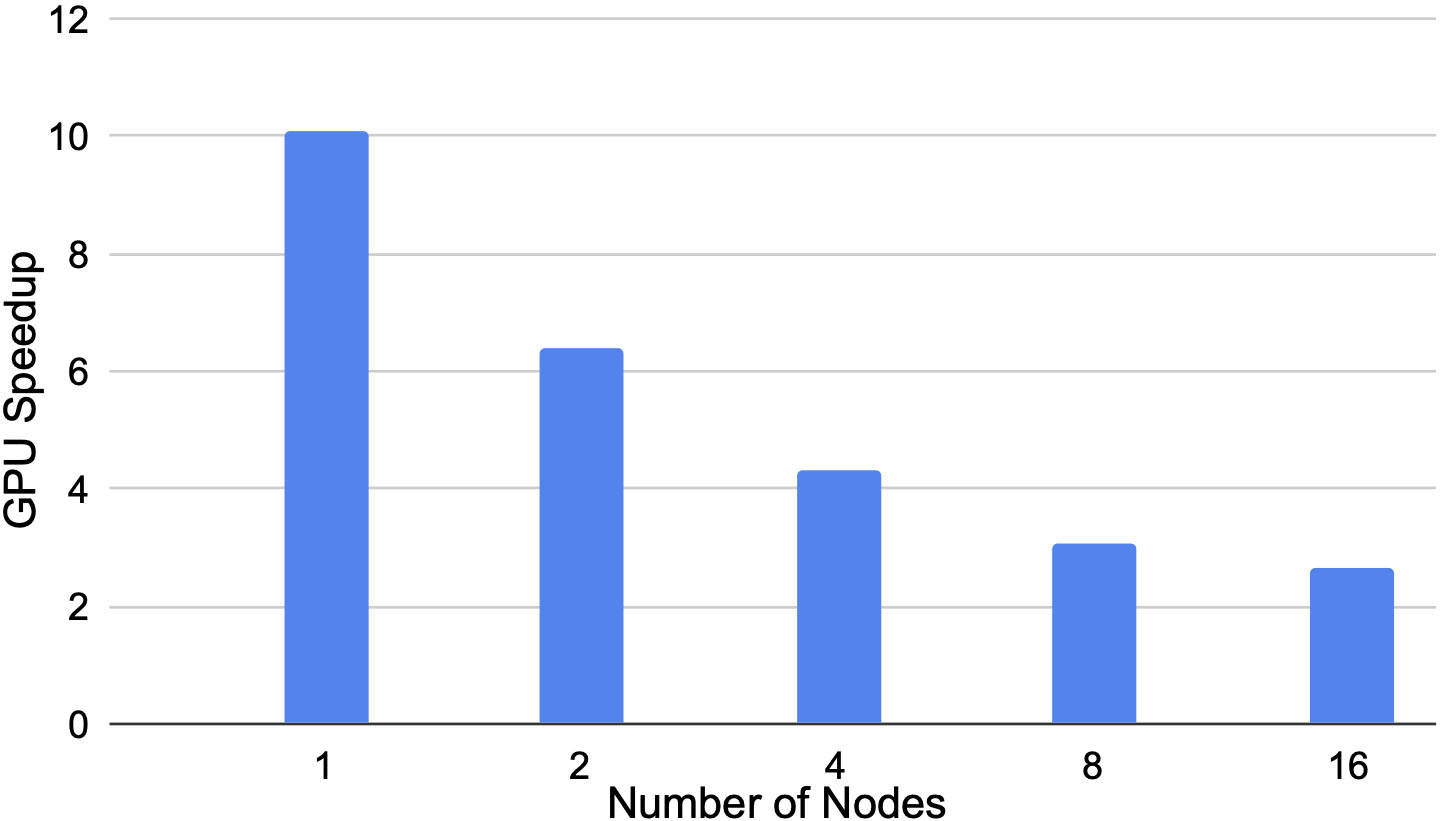
\includegraphics[width=0.8\textwidth]{fig_problem/vasp_gpu.jpg}
\caption{VASP GPU speedup for benchmark Si128 acfdtr. The horizontal axis shows the number of nodes, and the vertical axis shows the GPU speedup of VASP (Time(CPU)/Time(GPU)). (Recent unpublished benchmarks of VASP on NVIDIA A100 GPUs).}\label{fig:vasp_gpu}
\end{figure}


\begin{figure}[!h]
\centering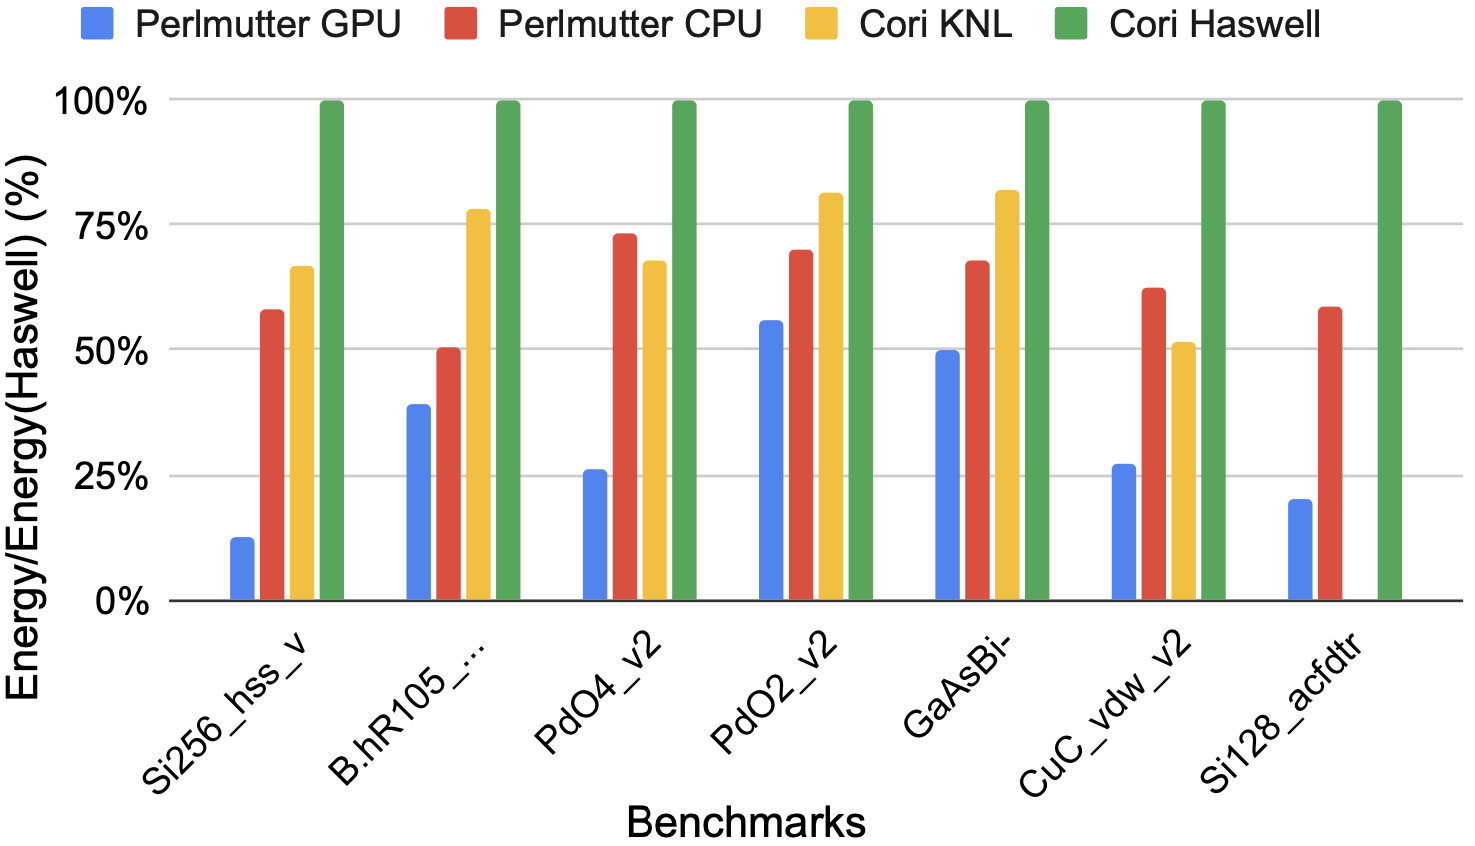
\includegraphics[width=0.8\textwidth]{fig_problem/vasp_energy.jpg}
\caption{Total energy usage comparison when running VASP on Perlmutter and Cori. The vertical axis shows the energy used by VASP benchmark jobs on Perlmutter GPUs (blue bars), CPUs (red bars), Cori KNL (yellow bars), and Cori Haswell (green bars) in ratio to the Cori Haswell usage. (Recent unpublished benchmarks of VASP on NVIDIA A100 GPUs).}\label{fig:vasp_energy}
\end{figure}


\subsubsection{Computational Chemistry}


\par
A great deal of computational resources are spent in Quantum Chemical calculations which involve the solution of the Hartree-Fock eigenvalue problem, which requires the diagonalization of the Fock matrix whose elements are given by:
\begin{eqnarray}\label{eq:hf_equation}
F_{\alpha\beta} = H_{\alpha\beta}^{core} + \sum_{\gamma\delta}D_{\gamma\delta}\Big[(\alpha\beta|\gamma\delta)-\frac{1}{2}(\alpha\delta|\gamma\beta)\Big] \,.
\end{eqnarray}


\par
The first term is related to the one electron contributions and the second term is related to the electron repulsion integrals (ERIs), in parenthesis, weighted by the by the density matrix $D_{\gamma\delta}$.
One of the most expensive parts in the solution of the Hartree-Fock equations is the processing (digestion) of the ERIs, one algorithm to do this task is shown in Fig.~\ref{fig:hf_algorithm}.


\begin{figure}[!h]
\centering
\includegraphics[width=0.4\textwidth]{fig_problem/hartree_fock_algorithms.png}
\caption{The pseudocode for a na\"ive ERI digestion algorithm~\cite{barca2021faster}.}\label{fig:hf_algorithm}
\end{figure}


\par
This algorithm is suitable for GPUs as it involves many arithmetic operations.
In addition to this, there are symmetries and properties of the integrals that could be used to rearrange the loops in an efficient manner that fit GPU architectures.


\subsubsection{Humanities}


\par
Below is a brief introduction into some of the work that is being done in the humanities that can benefit from utilizing GPUs.


\paragraph{Language models and NLP (natural language processing).}
With the recent popularity of ChatGPT, the use of language models has come into the mainstream, however such models have been used in the humanities many years already.
One of the biggest goals of humanities researchers is working with textual data which has increased exponentially over recent years due to the rise in social media.
Analyzing such textual data to gain insights into questions of sociology, linguistics and various other fields have become increasingly reliant on using language models.
Along with language models, the need for GPU access has become essential.


\paragraph{Archeology.}
The field of archeology also makes use of GPUs in their 3D modelling and rendering work.
The biggest problem with archeological sites is that once they are excavated, they are destroyed, so any researchers who aren’t present at the site, would lose valuable insights into how it looked when it was found.
However, with recent developments in technology and accessibility to high-performance computing, they are able to generate extremely detailed renderings of the excavation sites which act as a way to preserve the site for future researchers to gain critical insights and contribute to the research.


\paragraph{Cognitive Science.}
Techniques such as Markov Chain Monte Carlo (MCMC) sampling have proven to be invaluable in studies that delve into human behavior or population dynamics.
MCMC sampling allows researchers to simulate and analyze complex systems by iteratively sampling from a Markov chain, enabling the exploration of high-dimensional parameter spaces.
This method is particularly useful when studying human behavior, as it can capture the inherent randomness and interdependencies that characterize social systems.
By leveraging MCMC sampling, researchers can gain insights into various aspects of human behavior, such as decision-making, social interactions, and the spread of information or diseases within populations.


\par
By offloading the computational workload to GPUs, researchers can experience substantial speedup in the execution of MCMC algorithms.
This speedup allows for more extensive exploration of parameter spaces and facilitates the analysis of larger datasets, leading to more accurate and detailed insights into human behavior or population dynamics.
Examples of studies done using these methods can be found at the Center for Humanities Computing Aarhus (CHCAA) and Interacting Minds Centre (IMC) at Aarhus University.


\section{GPU Programming Concepts}


\subsection{Different types of parallelism}


\subsubsection{Distributed- vs. shared-memory architecture}


\par
Most of computing problems are not trivially parallelizable, which means that the subtasks need to have access from time to time to some of the results computed by other subtasks.
The way subtasks exchange needed information depends on the available hardware.
How the information/data exchange depending on the detailed computer architecture.


\par
As shown in Fig.~\ref{fig:distributed_vs_shared}, in a distributed memory environment each computing unit operates independently from the others.
It has its own memory and it cannot access the memory in other nodes.
The communication is done via network and each computing unit runs a separate copy of the operating system.
In a shared memory machine all computing units have access to the memory and can read or modify the variables within.


\begin{figure}[!h]
\centering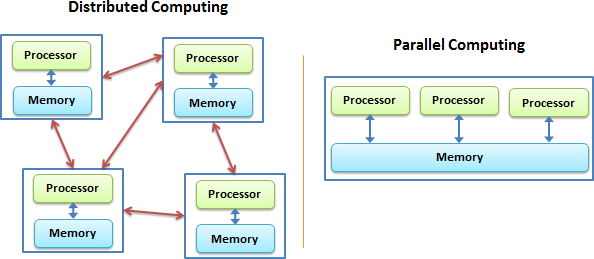
\includegraphics[width=0.8\textwidth]{fig_hardware/distributed_vs_shared.png}
\caption{Distributed- vs shared-memory parallel computing.}\label{fig:distributed_vs_shared}
\end{figure}


\subsubsection{Process-based and thread-based parallelism}


\par
The type of programming environment (distributed- or shared-memory) determines the programming model.
There are two types of parallelism,~\textbf{process-based parallelism} and~\textbf{thread-based parallelism}, as shown in Fig.~\ref{fig:process_thread_parallelism}.


\begin{figure}[!h]
\centering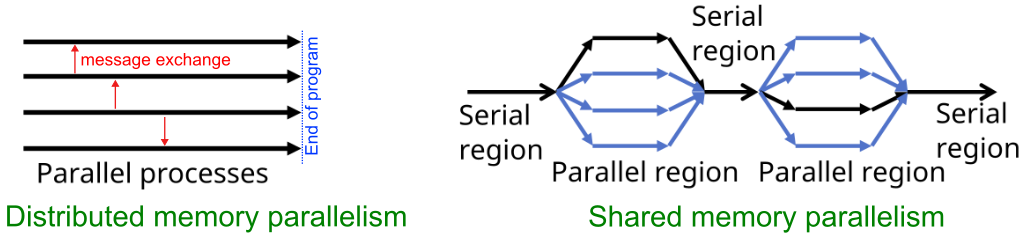
\includegraphics[width=0.8\textwidth]{fig_hardware/process_thread_parallelism.png}
\caption{The process-based and thread-based parallelism.}\label{fig:process_thread_parallelism}
\end{figure}


\par
For distributed memory machines, a process-based parallel programming model is employed.
The processes are independent execution units which have their own memory address spaces.
They are created when the parallel program is started and they are only terminated at the end.
The communication between them is done explicitly via message passing like~\textbf{MPI}.


\par
On the shared memory architectures it is possible to use a thread-based parallelism.
The threads are light execution units and can be created and destroyed at a relatively small cost.
The threads have their own state information but they share the same memory address space.
When needed the communication is done though the shared memory.


\par
Both approaches have their advantages and disadvantages.
Distributed machines are relatively cheap to build and they have an~\lq\lq infinite\rq\rq~capacity.
In principle one could add more and more computing units.
In practice the more computing units are used the more time consuming is the communication.
The shared memory systems can achieve good performance and the programming model is quite simple.
However they are limited by the memory capacity and by the access speed.
In addition in the shared parallel model it is much easier to create race conditions.


\subsubsection{Data and task parallelism}

\par
There are two types of parallelism that can be explored, as shown in Fig.~\ref{fig:data_task_parallelism}.
The data parallelism is when the data can be distributed across computational units that can run in parallel.
The units process the data by applying the same or very similar operation to different data elements.
A common example is applying a blur filter to an image --- the same function is applied to all the pixels on an image.
This parallelism is natural for the GPU, where the same instruction set is executed in multiple threads.


\begin{figure}[!h]
\centering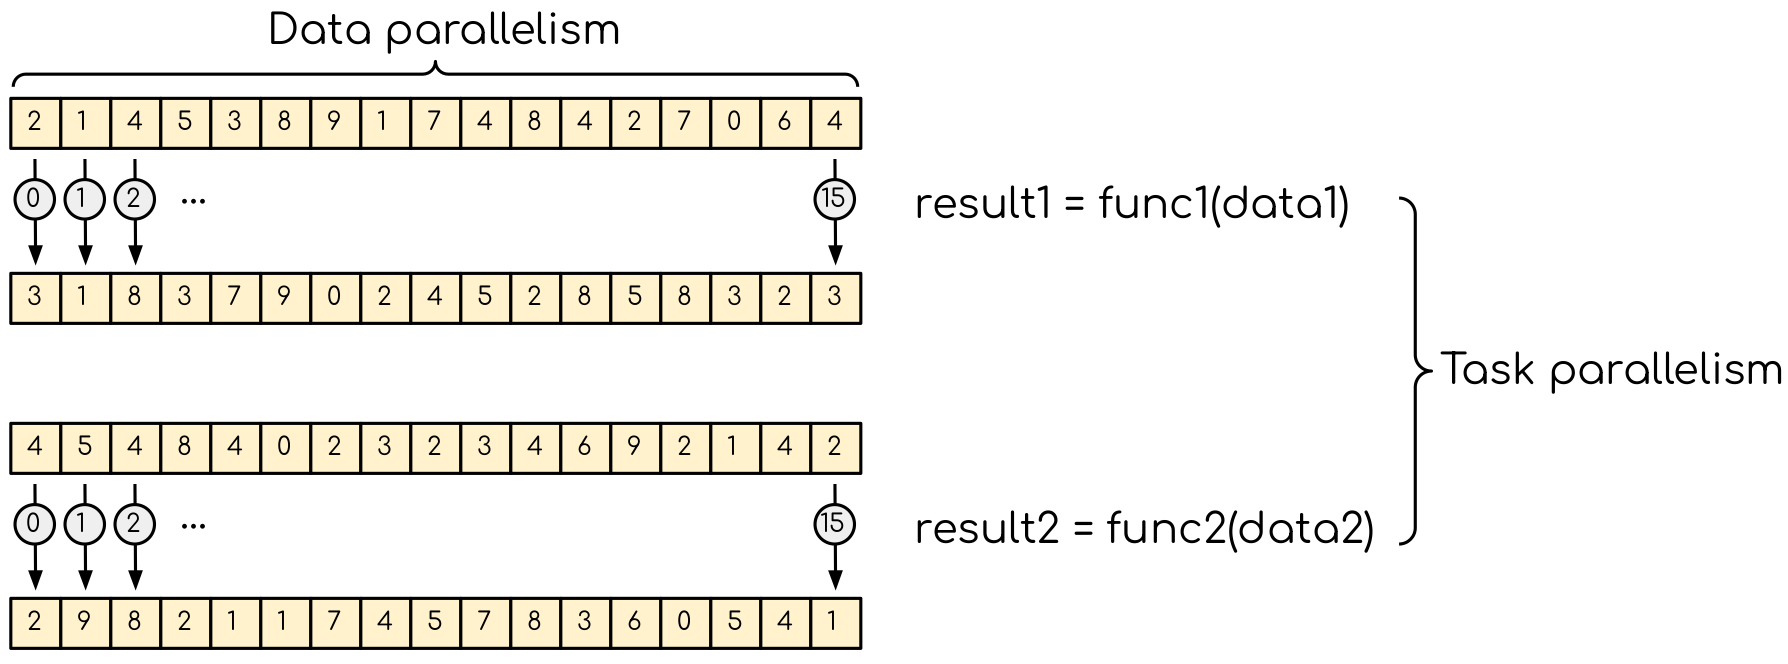
\includegraphics[width=0.8\textwidth]{fig_hardware/data_task_parallelism.png}
\caption{The data parallelism and task parallelism.}\label{fig:data_task_parallelism}
\end{figure}


\par
Data parallelism can usually be explored by the GPUs quite easily.
The most basic approach would be finding a loop over many data elements and converting it into a GPU kernel.
If the number of elements in the data set is fairly large (tens or hundred of thousands elements), the GPU should perform quite well.
Although it would be odd to expect absolute maximum performance from such a naive approach, it is often the one to take.
Getting absolute maximum out of the data parallelism requires good understanding of how GPU works.

\par
Another type of parallelism is the task parallelism.
This is when an application consists of more than one task that requiring to perform different operations with (the same or) different data.
An example of task parallelism is cooking: slicing vegetables and grilling are very different tasks and can be done at the same time.
Note that the tasks can consume totally different resources, which also can be explored.


\par
A short summary of this subsection:
\begin{itemize}
    \item Computing problems can be parallelized in distributed memory or shared memory architectures.
    \item In distributed memory, each unit operates independently, with no direct memory access between nodes.
    \item In shared memory, units have access to the same memory and can communicate through shared variables.
    \item Parallel programming can be process-based (distributed memory) or thread-based (shared memory).
    \item Process-based parallelism uses independent processes with separate memory spaces and explicit message passing.
    \item Thread-based parallelism uses lightweight threads that share the same memory space and communicate through shared memory.
    \item Data parallelism distributes data across computational units, processing them with the same or similar operations.
    \item Task parallelism involves multiple independent tasks that perform different operations on the same or different data.
    \item Task parallelism involves executing different tasks concurrently, leveraging different resources.
\end{itemize}


% -------------------------------------------------------------------- %


\subsection{GPU execution model}


\par
In order to obtain maximum performance it is important to understand how GPUs execute the programs (Fig.~\ref{fig:cpu_gpu_highway}).
As mentioned before a CPU is a flexible device oriented towards general purpose usage.
It’s fast and versatile, designed to run operating systems and various, very different types of applications.
It has lots of features, such as better control logic, caches and cache coherence, that are not related to pure computing.
CPUs optimize the execution by trying to achieve low latency via heavy caching and branch prediction.


\begin{figure}[!h]
\centering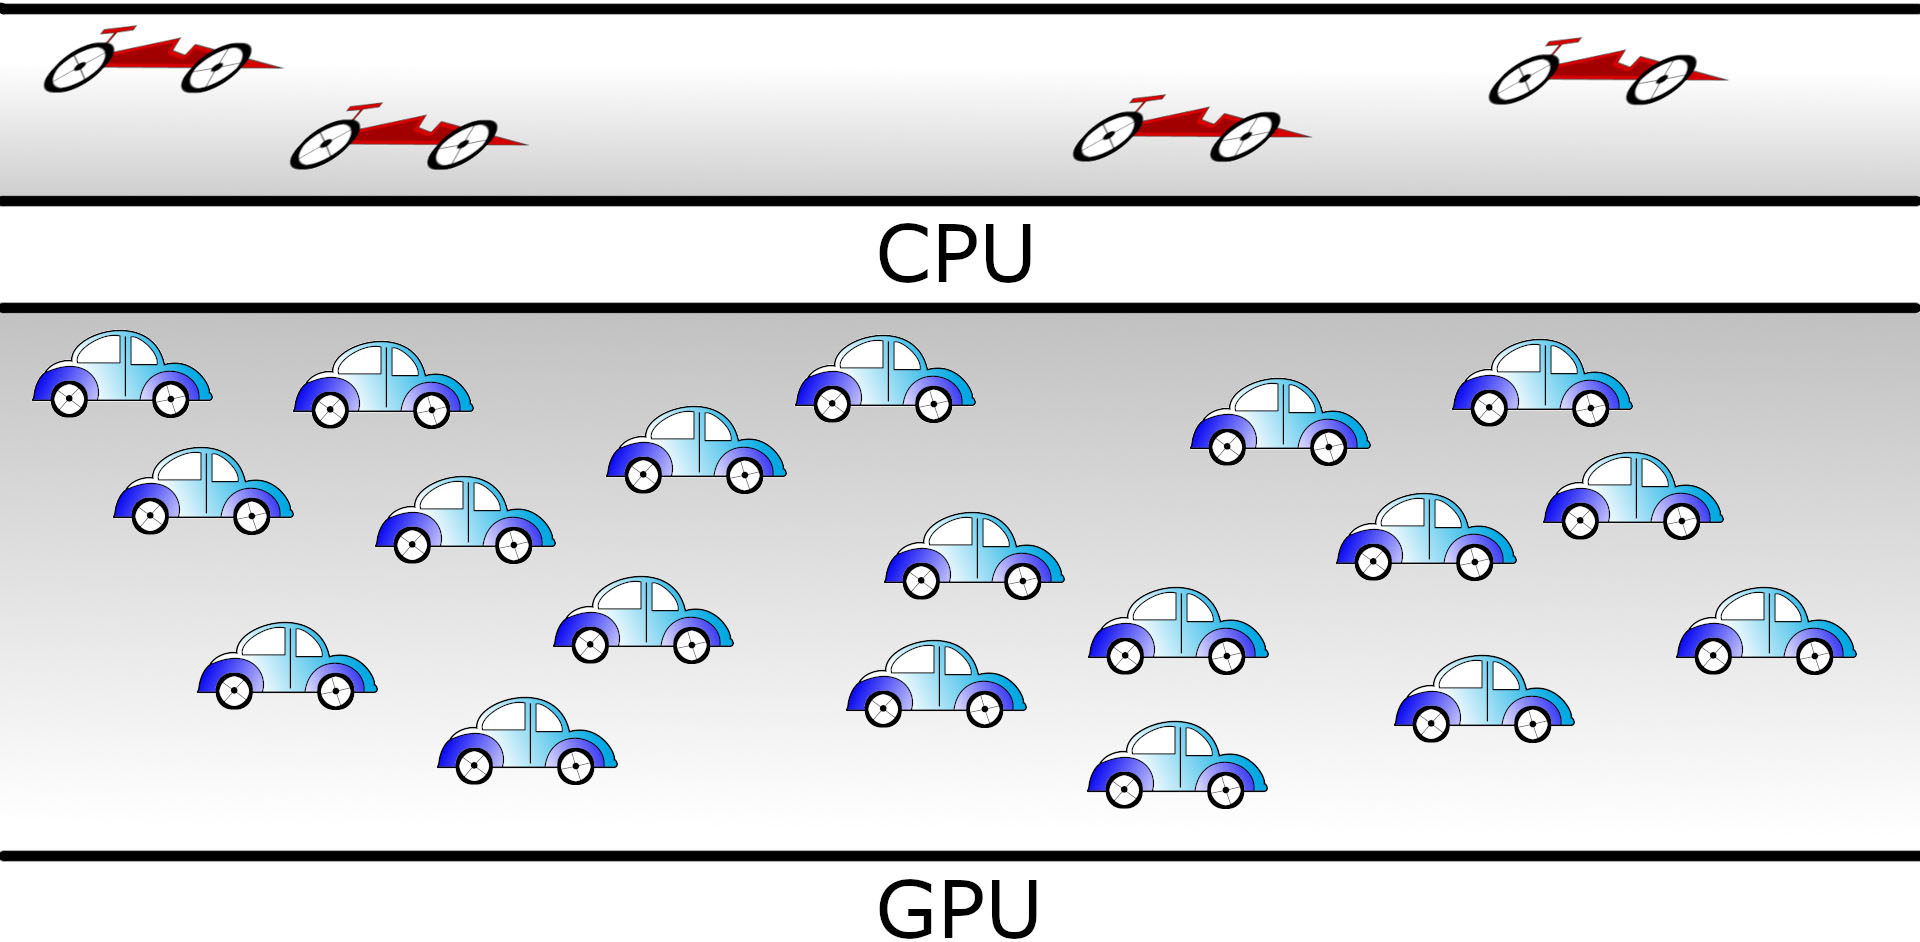
\includegraphics[width=0.8\textwidth]{fig_hardware/cpu_gpu_highway.jpg}
\caption{Cars and roads analogy for the CPU and GPU behavior. The compact road is analogous to the CPU (low latency, low throughput) and the broader road is analogous to the GPU (high latency, high throughput).}\label{fig:cpu_gpu_highway}
\end{figure}


\par
In contrast the GPUs contain a relatively small amount of transistors dedicated to control and caching, and a much larger fraction of transistors dedicated to the mathematical operations.
Since the cores in a GPU are designed just for 3D graphics, they can be made much simpler and there can be a very larger number of cores.
The current GPUs contain thousands of CUDA cores.
Performance in GPUs is obtain by having a very high degree of parallelism.
Lots of threads are launched in parallel.
For good performance there should be at least several times more than the number of CUDA cores.
GPU threads are much lighter than the usual CPU threads and they have very little penalty for context switching.
This way when some threads are performing some memory operations (reading or writing) others execute instructions.


\subsubsection{GPU threads}


\par
In order to perform some work the program launches a function called~\textbf{kernel}, which is executed simultaneously by tens of thousands of threads that can be run on GPU cores parallelly, as shown in Fig.~\ref{fig:thread_core}.
GPU threads are much lighter than the usual CPU threads and they have very little penalty for context switching.
By~\lq\lq over-subscribing\rq\rq~the GPU there are threads that are performing some memory operations (reading or writing), while others execute instructions.


\begin{figure}[!h]
\centering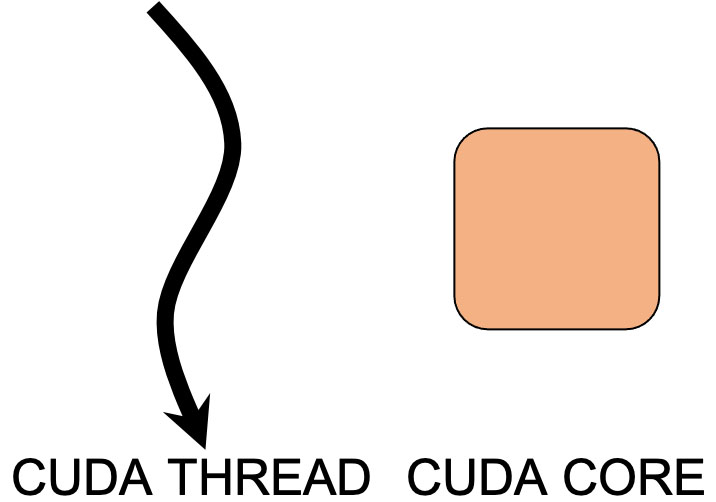
\includegraphics[width=0.5\textwidth]{fig_hardware/thread_core.jpg}
\caption{GPU Threads are executed on GPU cores}\label{fig:thread_core}
\end{figure}


\par
Every thread is associated with a particular intrinsic index which can be used to calculate and access memory locations in an array. 
Each thread has its context and set of private variables.
All threads have access to the global GPU memory, but there is no general way to synchronize when executing a kernel.
If some threads need data from the global memory which was modified by other threads the code would have to be splitted in several kernels because only at the completion of a kernel it is ensured that the writing to the global memory was completed.


\subsubsection{GPU warps}


\par
Apart from being much light weighted there are more differences between GPU threads and CPU threads.
GPU threads with consecutive thread indexes are bundled together in groups called~\textbf{warps}, as shown in Fig.~\ref{fig:warp_simt}.
This done at hardware level.


\begin{figure}[!h]
\centering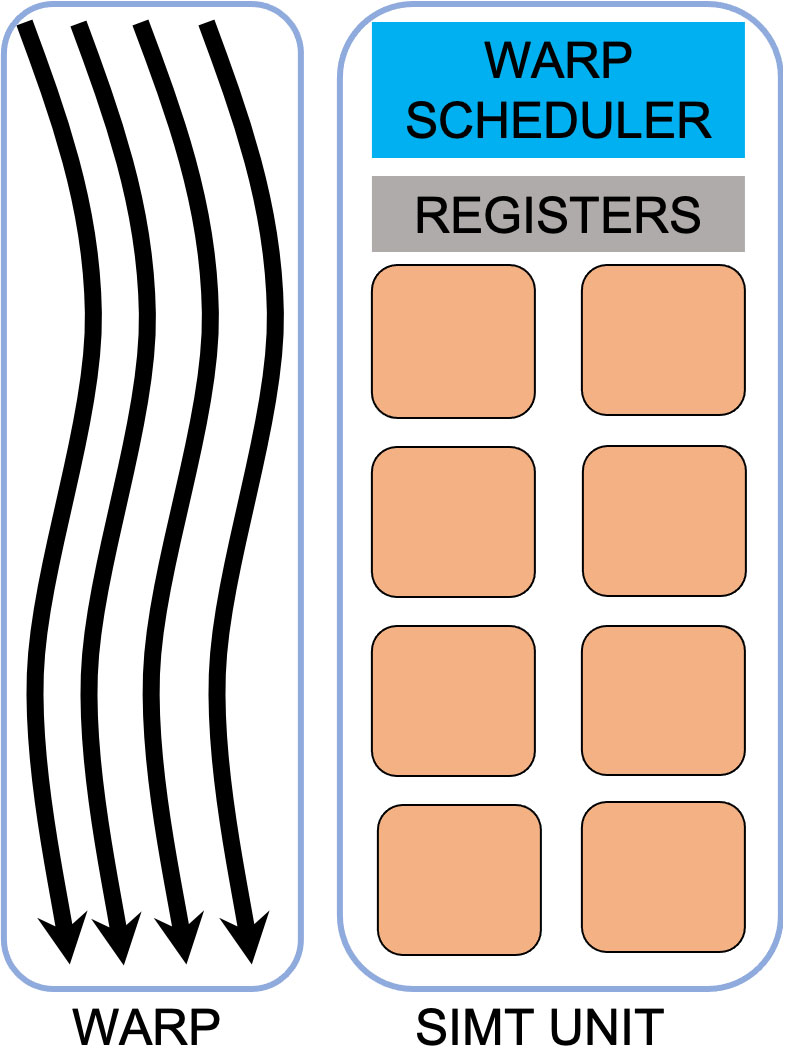
\includegraphics[width=0.4\textwidth]{fig_hardware/warp_simt.jpg}
\caption{Warp is the scheduling unit in SMs, and it executes in a SIMD manner.}\label{fig:warp_simt}
\end{figure}


\par
All memory accesses to the GPU memory are as a group in blocks of specific sizes (32B, 64B, 128B, $etc.$).
To obtain good performance, the CUDA threads in the same warp need to access elements of the data which are adjacent in the memory. 
This is called coalesced memory access.


\par
On some architectures, all members of a warp have to execute the same instruction, the so-called~\lq\lq lock-step\rq\rq~execution. 
This is done to achieve higher performance, but there are some drawbacks.
If an $if$-$else$ statement is present inside a warp will cause the warp to be executed more than once, one time for each branch.
When different threads within a single warp take different execution paths based on a conditional statement, both branches are executed sequentially, with some threads being active while others are inactive.
On architectures without lock-step execution, such as NVIDIA Volta/Turing ($e.g.$, GeForce 16xx-series) or newer, warp divergence is less costly.


\subsubsection{GPU blocks}


\par
There is another level in the GPU threads hierarchy. The threads are grouped together in so called~\textbf{blocks}.
Each block is assigned to one Streaming Multiprocessor (SMP) unit, as illustrated in Fig.~\ref{fig:block_smp}.
A SMP contains one or more SIMT (single instruction multiple threads) units, schedulers, and very fast on-chip memory.
Some of this on-chip memory can be used in the programs, this is called~\textbf{shared memory}.
The shared memory can be used to~\lq\lq cache\rq\rq~data that is used by more than one thread, thus avoiding multiple reads from the global memory.
It can also be used to avoid memory accesses which are not efficient.
For example in a matrix transpose operation, we have two memory operations per element and only can be coalesced.
In the first step a tile of the matrix is saved read a coalesced manner in the shared memory.
After all the reads of the block are done the tile can be locally transposed (which is very fast) and then written to the destination matrix in a coalesced manner as well.
Shared memory can also be used to perform block-level reductions and similar collective operations.
All threads can be synchronized at block level.
Furthermore when the shared memory is written in order to ensure that all threads have completed the operation the synchronization is compulsory to ensure correctness of the program.


\begin{figure}[!h]
\centering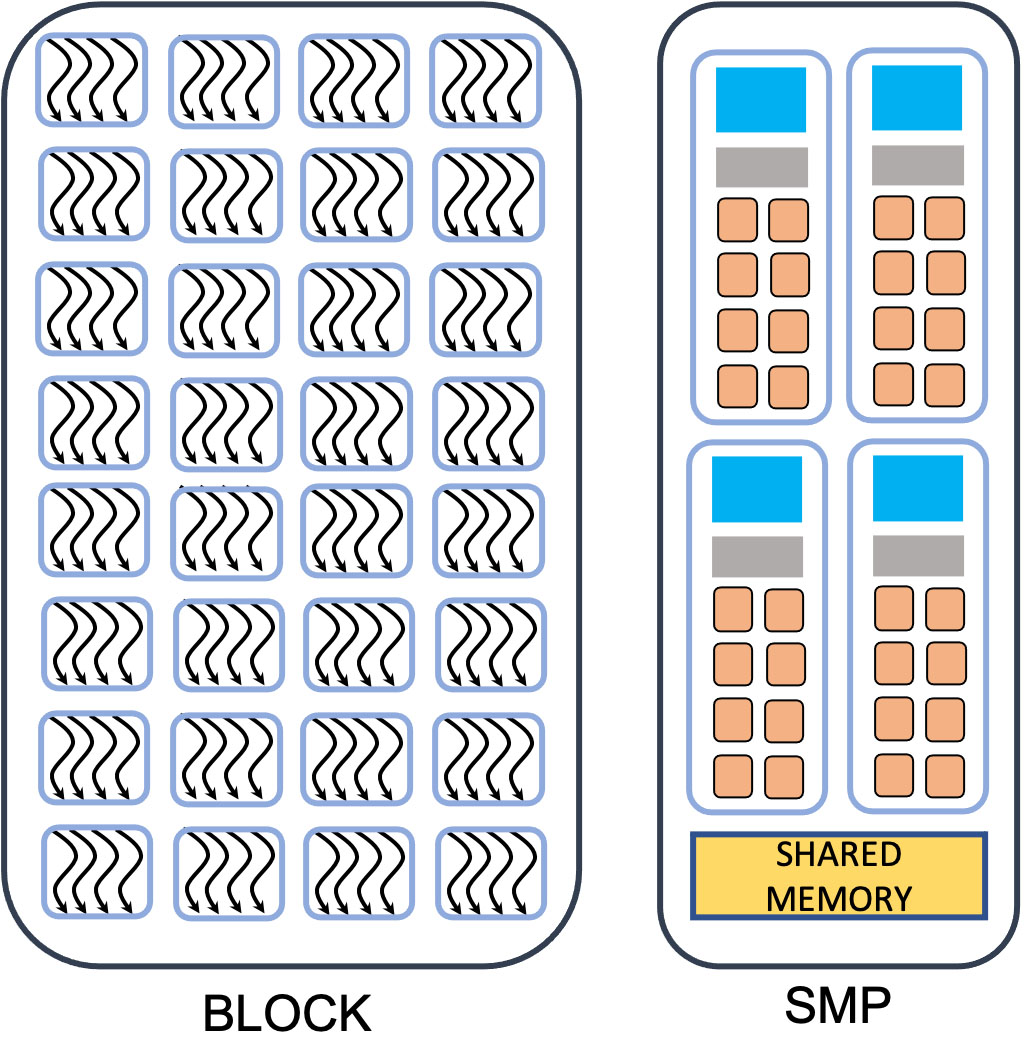
\includegraphics[width=0.5\textwidth]{fig_hardware/block_smp.jpg}
\caption{Each block is assigned to one SMP unit.}\label{fig:block_smp}
\end{figure}


\par
Finally, a block of threads can not be splitted among SMPs.
For performance blocks should have more than one warp.
The more warps are active on an SMP the better is hidden the latency associated with the memory operations.
If the resources are sufficient, due to fast context switching, an SMP can have more than one block active in the same time.
However these blocks can not share data with each other via the on-chip memory.


\par
In order to hide latencies it is recommended to~\lq\lq over-subscribe\rq\rq~the GPU.
There should be many more blocks than SMPs present on the device.
Also in order to ensure a good occupancy of the CUDA cores there should be more warps active on a given SMP than SIMT units.
This way while some warps of threads are idle waiting for some memory operations to complete, others use the CUDA cores, thus ensuring a high occupancy of the GPU.


\par
In addition to this there are some architecture-specific features of which the developers can take advantage.
Warp-level operations are primitives provided by the GPU architecture to allow for efficient communication and synchronization within a warp.
They allow threads within a warp to exchange data efficiently, without the need for explicit synchronization.
These warp-level operations, combined with the organization of threads into blocks and clusters, make it possible to implement complex algorithms and achieve high performance on the GPU.
The cooperative groups feature introduced in recent versions of CUDA provides even finer-grained control over thread execution, allowing for even more efficient processing by giving more flexibility to the thread hierarchy. Cooperative groups allow threads within a block to organize themselves into smaller groups, called cooperative groups, and to synchronize their execution and share data within the group.


\subsubsection{Mapping thread and thread block to elements of an array}


\par
In CUDA, a grid refers to the collection of thread blocks that together form the entire set of parallel work to be executed on a GPU. 
A CUDA grid is organized in a one-, two-, or three-dimensional structure, depending on the problem and data organization.
The dimensions of the grid determine how the blocks are arranged in the grid.
For example, a one-dimensional grid has a linear arrangement of blocks, while a two-dimensional grid forms a grid-like structure with rows and columns of blocks.


\par
Within a grid, individual blocks are organized in a one-, two-, or three-dimensional arrangement as well.
Each block consists of multiple threads that execute concurrently.
The dimensions of a block determine how threads are arranged within the block.
A one-dimensional block has threads arranged linearly, while a two-dimensional block has a grid-like arrangement of threads.


\par
To execute a grid of threads on the GPU, a CUDA kernel function is launched.
The kernel function defines the code that will be executed by each thread within the grid.
When launching a CUDA kernel, the size of the grid (the number of blocks) and the size of each block (the number of threads) should be clearly specified.
Within the kernel function, each thread can determine its unique index within the grid using built-in variables provided by CUDA.
For example, the variables $threadIdx.x$, $threadIdx.y$, and $threadIdx.z$ represent the thread's index within its block, while $blockIdx.x$, $blockIdx.y$, and $blockIdx.z$ represent the block's index within the grid.
The combination of these indices allows each thread to compute its unique global index within the entire grid.


\par
Fig.~\ref{fig:thread_block_index} presents an example of how the threads in a grid can be associated with specific elements of an array.
The thread marked by orange color is part of a grid of threads size 4096.
The threads are grouped in blocks of size 256.
The~\lq\lq orange\rq\rq~thread has index 3 in the block 2 and the global calculated index 515.
For a vector addition example this would be used as follow $c[index] = a[index] + b[index]$.


\begin{figure}[htbp]
\centering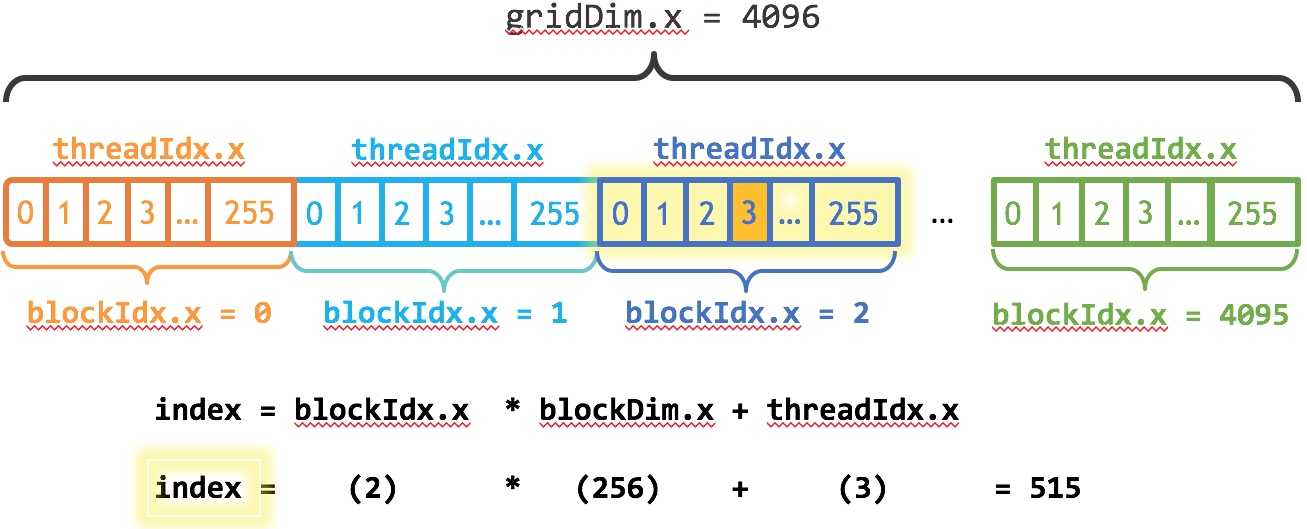
\includegraphics[width=0.8\textwidth]{fig_hardware/thread_block_index.png}
\caption{An example of the CUDA Indexing Pattern. $gridDim.x$ is the number of blocks, $blockDim.x$ is the number of threads in each block, $blockIdx.x$ is the index of the current block within the grid, and $threadIdx.x$ is the index of the current thread inside the block~\cite{indexing}.}\label{fig:thread_block_index}
\end{figure}


\par
To summarize this section.
\begin{itemize}
    \item GPUs have a distinct execution model compared to CPUs, with a focus on parallelism and mathematical operations.
    \item GPUs consist of thousands of lightweight threads that can be executed simultaneously on GPU cores.
    \item Threads are organized into warps, and warps are grouped into blocks assigned to streaming multiprocessors (SMPs).
    \item GPUs achieve performance through high degrees of parallelism and efficient memory access.
    \item Shared memory can be used to cache data and improve memory access efficiency within a block.
    \item Synchronization and data sharing are limited to the block level, with some possible sharing at the warp level depending on the architecture.
    \item Over-subscribing the GPU and maximizing warp and block occupancy help hide latencies and improve performance.
    \item Warp-level operations and cooperative groups provide efficient communication and synchronization within a warp or block.
    \item Thread indexing allows associating threads with specific elements in an array for parallel processing.
\end{itemize}


% -------------------------------------------------------------------- %


\subsection{GPU Terminology}


\par
At the moment there are three major GPU producers: NVIDIA, Intel, and AMD.
While the basic concept behind GPUs is pretty similar they use different names for the various parts.
Furthermore there are software environments for GPU programming, some from the producers and some from external groups all having different naming as well.
In Table~\ref{tbl:gpu_terminology_cuda_hip_opencl_sycl}, there is a short compilation of the some terms used across different platforms and software environments.


\begin{table}[h]
\begin{center}
\begin{threeparttable}\caption{Software mapping naming.}\label{tbl:gpu_terminology_cuda_hip_opencl_sycl}
\begin{tabular}{ |c@{\quad}|c@{\quad}|c@{\quad}|c@{\quad}| } 
\hline
\textbf{CUDA} & \textbf{HIP} & \textbf{OpenCL} & \textbf{SYCL} \\
\hline
\multicolumn{2}{|c|}{grid of threads} & \multicolumn{2}{c|}{NDRange} \\ \hline
\multicolumn{2}{|c|}{block} & \multicolumn{2}{c|}{work-group} \\ \hline
warp & wavefront & \multicolumn{2}{c|}{sub-group} \\ \hline
\multicolumn{2}{|c|}{thread} & \multicolumn{2}{|c|}{work-item} \\ \hline
\multicolumn{2}{|c|}{registers} & \multicolumn{2}{|c|}{private memory} \\ \hline
shared memory & local data share & \multicolumn{2}{|c|}{local memory} \\ \hline
\multicolumn{2}{|c|}{threadIdx.\{x,y,z\}} & get\_local\_id({0,1,2}) & nd\_item::get\_local({2,1,0})\tnote{**} \\ \hline
\multicolumn{2}{|c|}{blockIdx.{x,y,z}} & get\_group\_id({0,1,2}) & nd\_item::get\_group({2,1,0})\tnote{**} \\ \hline
\multicolumn{2}{|c|}{blockDim.{x,y,z}} & get\_local\_size({0,1,2}) & nd\_item::get\_local\_range({2,1,0})\tnote{**} \\
\hline
\end{tabular}
\begin{tablenotes}
\item[**] (1,2,3) In SYCL, the thread indexing is inverted. In a 3D grid, physically adjacent threads have consecutive X(0) index in CUDA, HIP, and OpenCL, but consecutive Z(2) index in SYCL. In a 2D grid, CUDA, HIP, and OpenCL still has contiguous indexing along X(0) dimension, while in SYCL it is Y(1). Same applies to block dimensions and indexing.
\end{tablenotes}
\end{threeparttable}
\end{center}
\end{table}


\section{Introduction to GPU Programming Models}


\par
There are different ways to use GPUs for computations.
In the best case, when someone has already written the code, one only needs to set the parameters and initial configurations in order to get started.
Or in some cases the problem is in such a way that it is only needed to use a library to solve the most intensive part of the code.
However these are quite limited cases and in general some programming might be needed.
There are several GPU programming software environments and APIs available, such as~\textbf{directive-based models},~\textbf{non-portable kernel-based models}, and~\textbf{portable kernel-based models}, as well as~\textbf{high-level frameworks and libraries}.
Below provides a general explanation of these contents, and the detailed description of these contents will be illustrated in the following sections.


\subsection{Standard C++/Fortran}


\par
Programs written in standard C++ and Fortran languages can now take advantage of NVIDIA GPUs without depending of any external library.
This is possible thanks to the NVIDIA Software Development Kit (SDK), which provides a suite of compilers~\cite{NVIDIA_SDK} that translates and optimizes the code for running on GPUs.
Guidelines for writing C++ and Fortran code are available at the community for developers using NVIDIA GPUs~\cite{guideline_gpu_cpp, guideline_gpu_fortran}.
The performance of these two approaches is promising as it can be seen in the examples provided in those guidelines.


% -------------------------------------------------------------------- %


\subsection{Directive-based programming}


\par
A fast and cheap way is to use directive based approaches.
In this case the existing serial code is annotated with hints which indicate to the compiler which loops and regions should be executed on the GPU.
In the absence of the API the directives are treated as comments and the code will just be executed as a usual serial code.
This approach is focused on productivity and easy usage (but to the detriment of performance), and allows employing accelerators with minimum programming effort by adding parallelism to existing code without the need to write accelerator-specific code.
There are two common ways to program using directives, namely~\textbf{OpenACC} and~\textbf{OpenMP}.


\subsubsection{OpenACC}

\par
OpenACC (Open Accelerator)~\cite{openacc} is developed by a consortium formed in 2010 with the goal of developing a standard, portable, and scalable programming model for accelerators, including GPUs.
Members of the OpenACC consortium include GPU vendors, such as NVIDIA and AMD, as well as leading supercomputing centers, universities, and software companies.
Until recently it was supporting only NVIDIA GPUs, but now there is effort to support more and more devices and architectures.


\par
OpenACC provides directives, compiler directives, and APIs that enable developers to annotate existing code and offload computationally intensive portions to accelerators while maintaining portability across different platforms.
OpenACC relies on compiler directives to express parallelism and data management.
Directives are pragmas or comments inserted into the source code to guide the compiler in parallelizing and optimizing the code.
These directives indicate which parts of the code should be offloaded to an accelerator, such as a GPU, and how to distribute the workload for loop parallelization, data mapping, data privatization, and loop collapsing, among others.


\subsubsection{OpenMP}


\par
OpenMP (Open Multi-Processing)~\cite{openmp} is a multi-platform and shared-memory parallel programming API.
It provides a scalable approach to parallel computing on multi-core CPUs, and adds relatively recently support for GPU offloading.
It aims to support various types of GPUs.


\par
OpenMP also uses compiler directives, typically in the form of pragmas, to express parallelism and guide the compiler in parallelizing the code.
Directives are inserted into the source code to indicate which sections or loops should be executed in parallel.
These directives enable developers to parallelize their code by adding directives and library calls, enabling the execution of multiple threads to work on different parts of the code simultaneously.


\par
OpenMP is widely supported across different compilers, platforms, and programming languages, including C/C++ and Fortran.
In these three programming languages, you can control the level of parallelism, specify loop scheduling, handle reductions, and use other OpenMP constructs to optimize and control parallel execution.


% -------------------------------------------------------------------- %


\subsection{Non-portable kernel-based models}


\par
When doing direct GPU programming the developer has a large level of control by writing low-level code that directly communicates with the GPU and its hardware.
Theoretically direct GPU programming methods provide the ability to write low-level, GPU-accelerated code that can provide significant performance improvements over CPU-only code.
However, they also require a deeper understanding of the GPU architecture and its capabilities, as well as the specific programming method being used.
Multiple examples of CUDA/HIP code are available in the~\textbf{\textcolor{brown}{content/examples/cuda-hip}} directory of this repository~\cite{gpu-programming-examples}.


\par
Non-portable kernel-based models refer to native computational models or algorithms that are specifically designed and implemented for a particular hardware architecture or platform.
These models heavily rely on low-level optimizations and hardware-specific features, making them non-portable across different architectures or systems.
The advantage of non-portable kernel-based models is the potential for achieving highly optimized and efficient computations on specific hardware architectures.
These models can exploit fine-grained parallelism, utilize hardware-specific features, and leverage low-level optimizations.
Representatives are CUDA (for NVIDIA GPUs) and HIP (for AMD GPUs).


\subsubsection{CUDA}

\par
CUDA~\cite{cuda} is a parallel computing platform and API developed by NVIDIA.
It is historically the first mainstream GPU programming framework.
It allows developers to write C++-like code that is executed on the GPU.
CUDA provides a set of libraries, compilers, and development tools for low-level GPU programming and provides a performance boost for demanding computationally-intensive applications.
While there is an extensive ecosystem, CUDA is restricted to NVIDIA hardware.


\subsubsection{HIP}


\par
HIP (Heterogeneous-compute Interface for Portability)~\cite{hip} is a C++ programming language and runtime API developed by AMD that provides a low-level interface for GPU programming.
HIP is designed to provide a single source code that can be used on both NVIDIA and AMD GPUs.
It is based on the CUDA programming model and provides an almost identical programming interface to CUDA.


% -------------------------------------------------------------------- %


\subsection{Portable kernel-based models}

\par
Cross-platform portability ecosystems typically provide a higher-level abstraction layer which provide a convenient and portable kernel-based programming models for GPU programming.
They can help reduce the time and effort required to maintain and deploy GPU-accelerated applications.
The goal of these ecosystems is achieving performance portability with a single-source application.
In C++, the most notable cross-platform portability ecosystems are~\textbf{Alpaka}~\cite{alpaka},~\textbf{Kokkos}~\cite{kokkos},~\textbf{OpenCL} (C and C++ APIs)~\cite{OpenCL},~\textbf{RAJA}~\cite{raja}, and~\textbf{SYCL}~\cite{sycl}.


\subsubsection{Kokkos}


\par
Kokkos~\cite{kokkos} is an open-source performance portable programming model for heterogeneous parallel computing that has been so far mostly developed at Sandia National Laboratories.
It is a C++-based ecosystem that provides a programming model for developing efficient and scalable parallel applications that run on many-core architectures such as CPUs, GPUs, and FPGAs.
The Kokkos ecosystem consists of several components, such as the Kokkos core library, which provides parallel execution and memory abstraction, the Kokkos kernels library, which provides math kernels for linear algebra and graph algorithms, and the Kokkos tools library, which provides profiling and debugging tools.
Kokkos components integrate well with other software libraries and technologies, such as MPI and OpenMP. 
Furthermore, the project collaborates with other projects, in order to provide interoperability and standardization for portable C++ programming.


\subsubsection{OpenCL}


\par
OpenCL (Open Computing Language)~\cite{OpenCL} is a cross-platform, open-standard API for general-purpose parallel computing on CPUs, GPUs and FPGAs.
It supports a wide range of hardware from multiple vendors.
OpenCL provides a low-level programming interface for GPU programming and enables developers to write programs that can be executed on a variety of platforms.
Unlike programming models such as CUDA, HIP, Kokkos and SYCL, the OpenCL uses a separate-source model.
Recent versions of the OpenCL standard added C++ support for both API and the kernel code, but the C-based interface is still more widely used.
The OpenCL Working Group doesn’t provide any frameworks of its own. Instead, vendors who produce OpenCL-compliant devices release frameworks as part of their SDKs.
The two most popular OpenCL SDKs are released by NVIDIA and AMD.
In both cases, the development kits are free and contain the libraries and tools that make it possible to build OpenCL applications.


\subsubsection{SYCL}


\par
SYCL~\cite{sycl} is a royalty-free, open-standard C++ programming model for multi-device programming.
It provides a high-level, single-source programming model for heterogeneous systems, including GPUs. 
Originally SYCL was developed on top of OpenCL, however it is not limited to just that.
It can be implemented on top of other low-level heterogeneous computing APIs, such as CUDA or HIP, enabling developers to write programs that can be executed on a variety of platforms.
Note that while SYCL is relatively high-level model, the developers are still required to write GPU kernels explicitly.


\par
While Alpaka~\cite{alpaka}, Kokkos~\cite{kokkos}, and RAJA~\cite{raja} refer to specific projects, SYCL itself is only a standard, for which several implementations exist.
For GPU programming, Intel oneAPI DPC++~\cite{oneapi-dpc} (supporting Intel GPUs natively, and NVIDIA and AMD GPUs with Codeplay oneAPI plugins~\cite{codeplay-oneapi}) and hipSYCL~\cite{hipsycl} (also known as Open SYCL, supporting NVIDIA and AMD GPUs, with experimental Intel GPU support available in combination with Intel oneAPI DPC++) are the most widely used. 
Other implementations of note are triSYCL~\cite{trisycl} and ComputeCPP~\cite{computecpp}.


% -------------------------------------------------------------------- %


\subsection{High-level language-based programming}


\par
GPU programming traditionally relied on low-level languages like CUDA and OpenCL, which required explicit management of memory, thread synchronization, and other low-level details.
As GPUs became more widely adopted for general-purpose computing, high-level language support for GPU programming has also emerged.
Below are representative high-level languages that provide support for GPU programming.


\subsubsection{Python}

\par
Python offers support for GPU programming through several libraries, including:
\begin{itemize}
    \item~\textbf{CuPy}: CuPy~\cite{cupy} is a GPU-based data array library compatible with~\textbf{NumPy}/\textbf{SciPy}. It offers a highly similar interface to NumPy and SciPy, making it easy for developers to transition to GPU computing. To utilize CuPy, simply replace $numpy$ and $scipy$ with $cupy$ and $cupyx.scipy$ in your Python code.
    \item~\textbf{cuDF}: RAPIDS~\cite{rapids} is a high level package collections which implement CUDA functionalities and API with Python bindings. cuDF~\cite{cudf} belongs to RAPIDS and is the library for manipulating data frames on GPU. cuDF provides a pandas-like API, so if you are familiar with Pandas~\cite{pandas}, you can accelerate your work without knowing too much CUDA programming.
    \item~\textbf{PyCUDA}: PyCUDA~\cite{pycuda} is a Python programming environment for CUDA. It allows users to access to NVIDIA’s CUDA API from Python. PyCUDA is powerful library but only runs on NVIDIA GPUs. Knowledge of CUDA programming is needed.
    \item~\textbf{Numba}: Similarly as for CPUs, Numba~\cite{numba} allows users to just-in-time~\cite{jit} (JIT) compile Python code to work on GPU as well. Numba supports GPUs from NVIDIA and will likely support AMD GPUs in the future.
    \item~\textbf{PyTorch}: PyTorch~\cite{pytorch} is a deep learning framework that allows seamless integration with GPUs. It provides tensor operations and automatic differentiation capabilities, enabling efficient GPU-accelerated neural network training and inference.
    \item~\textbf{TensorFlow}: TensorFlow~\cite{tensorflow} is another widely used deep learning framework that supports GPU acceleration. It provides a high-level API for defining and training neural networks and takes advantage of GPUs to accelerate computations.
\end{itemize}


\subsubsection{Julia}


\par
Julia~\cite{julia} is a high-level, dynamic programming language designed for numerical and scientific computing.
It offers built-in support for parallel and distributed computing, including GPU acceleration.
Julia has first-class support for GPU programming through the following packages that target GPUs from all three major vendors:
\begin{itemize}
    \item~\textbf{\textcolor{brown}{CUDA.jl}} for NVIDIA GPUs~\cite{cudajl}
    \item~\textbf{\textcolor{brown}{AMDGPU.jl}} for AMD GPUs~\cite{amdgpujl}
    \item~\textbf{\textcolor{brown}{oneAPI.jl}} for Intel GPUs~\cite{oneapijl}
    \item~\textbf{\textcolor{brown}{Metal.jl}} for Apple M-series GPUs~\cite{metaljl}
\end{itemize}

\par
\textbf{\textcolor{brown}{CUDA.jl}} is the most mature,~\textbf{\textcolor{brown}{AMDGPU.jl}} is somewhat behind but still ready for general use, while~\textbf{\textcolor{brown}{oneAPI.jl}} and~\textbf{\textcolor{brown}{Metal.jl}} are functional but might contain bugs, miss some features and provide suboptimal performance.
Their respective APIs are however completely analogous and translation between libraries is straightforward.
All packages offer both high-level abstractions that require very little programming effort and a lower level approach for writing kernels for fine-grained control.


\subsubsection{Other high-level programming language}


Besides Python and Julia, there are other high-level language support GPU programming, such as~\textbf{MATLAB} and~\textbf{R}.
\begin{itemize}
    \item MATLAB: MATLAB~\cite{matlab} is a popular programming environment for numerical computing. It provides support for GPU computing through the Parallel Computing Toolbox. MATLAB allows users to perform computations on GPUs by utilizing GPU-enabled functions and leveraging the CUDA programming language under the hood.
    \item R: R~\cite{rproject} is a language widely used in statistical computing and data analysis. GPU acceleration is available for certain operations in R through packages such as~\textbf{gputools} and~\textbf{gpuR}. These packages provide functions that allow users to offload computations to GPUs and leverage parallel processing capabilities.
\end{itemize}


\par
It's important to note that while these high-level languages offer GPU programming support, they still rely on lower-level GPU programming frameworks or libraries underneath (such as CUDA or OpenCL) to communicate with the GPU and perform the actual parallel computations.
However, the high-level language interfaces simplify the development process and provide a more user-friendly experience for GPU programming.


% -------------------------------------------------------------------- %


\subsection{Summary}


\par
Each of these GPU programming environments has its own strengths and weaknesses, and the best choice for a given project will depend on a range of factors, including:
\begin{itemize}
    \item the hardware platforms being targeted
    \item the type of computation being performed, and
    \item the developer’s experience and preferences.
\end{itemize}


\par
\textbf{High-level and productivity-focused APIs} provide a simplified programming model and maximize code portability, while~\textbf{low-level and performance-focused APIs} provide a high level of control over the GPU’s hardware but also require more coding effort and expertise.


\begin{itemize}
    \item \textbf{Directive-based programming}:
    \begin{itemize}
        \item Existing serial code is annotated with directives to indicate which parts should be executed on the GPU.
        \item OpenACC and OpenMP are common directive-based programming models.
        \item Productivity and easy usage are prioritized over performance.
        \item Minimum programming effort is required to add parallelism to existing code.
    \end{itemize}
    \item \textbf{Non-portable kernel-based models}:
    \begin{itemize}
        \item Low-level code is written to directly communicate with the GPU.
        \item CUDA is NVIDIA’s parallel computing platform and API for GPU programming.
        \item HIP is an API developed by AMD that provides a similar programming interface to CUDA for both NVIDIA and AMD GPUs.
        \item Deeper understanding of GPU architecture and programming methods is needed.
    \end{itemize}
    \item \textbf{Portable kernel-based models}:
    \begin{itemize}
        \item Higher-level abstractions for GPU programming that provide portability.
        \item Examples include Alpaka, Kokkos, OpenCL, RAJA, and SYCL.
        \item Aim to achieve performance portability with a single-source application.
        \item Can run on various GPUs and platforms, reducing the effort required to maintain and deploy GPU-accelerated applications.
    \end{itemize}
    \item \textbf{High-level language-based programming}:
    \begin{itemize}
        \item Python libraries like CuPy, cuDF, PyCUDA, and Numba offer GPU programming capabilities.
        \item Julia has packages such as CUDA.jl, AMDGPU.jl, oneAPI.jl, and Metal.jl for GPU programming.
        \item These libraries provide high-level abstractions and interfaces for GPU programming in their respective languages.
    \end{itemize}
\end{itemize}

\section{High-Level Language-Based Programming}


\subsection{Python}


\par
There has been a lot of progress in GPU programming using Python and the ecosystem is still evolving.
There are a couple of options available to work with GPU.


\subsubsection{CuPy}


\par
CuPy~\cite{cupy} is a NumPy/SciPy-compatible data array library used on GPU.
It has been developed for NVIDIA GPUs but as experimental support for AMD GPUs.
CuPy has a highly compatible interface with NumPy and SciPy.
As stated on its official website,~\textit{\lq\lq All you need to do is just replace numpy and scipy with cupy and cupyx.scipy in your Python code\rq\rq}.
If you know NumPy, CuPy is a very easy way to get started on the GPU.


\subsubsection{cuDF}


\par
RAPIDS~\cite{rapids} is a high level packages collections which implement CUDA functionalities and API with Python bindings.
It only supports NVIDIA GPUs.
cuDF~\cite{cudf} belongs to RAPIDS and is the library for manipulating data frames on GPU.
cuDF provides a pandas-like API, so if you are familiar with Pandas~\cite{pandas}, you can accelerate your work without knowing too much CUDA programming.


\subsubsection{PyCUDA}


\par
PyCUDA~\cite{pycuda} is a Python programming environment for CUDA.
It allows users to access to NVIDIA’s CUDA API from Python.
PyCUDA is powerful library but only runs on NVIDIA GPUs.
Knowledge of CUDA programming is needed.


\subsubsection{Numba}


\par
Numba~\cite{numba} allows users to JIT~\cite{jit} compile Python code to run fast on CPUs, but can also be used for JIT compiling for GPUs.
In the following we will focus on using Numba, which supports GPUs from both NVIDIA and AMD.
It should be noted that Numba supported AMD GPUs up until version 0.53 but has since deprecated the support.


\par
Numba supports GPU programming by directly compiling a restricted subset of Python code into kernels and device functions following the execution model.
Kernels written in Numba appear to have direct access to NumPy arrays.
NumPy arrays are transferred between the CPU and the GPU automatically.


\par
Using~\textbf{ufuncs} (and generalized ufuncs (\textbf{gufunc})) is the easiest way to run on a GPU with Numba, and it requires minimal understanding of GPU programming.
Numba~\textbf{\textcolor{red}{@vectorize}} will produce a ufunc-like object.
This object is a close analog but not fully compatible with a regular NumPy ufunc.
Generating a ufunc for GPU requires the explicit type signature and target attribute.


\paragraph{Numba ufunc.}
Here are multiple samples for a simple mathematical problem using Numba~\textbf{ufunc} for CPU (List~\ref{lst:06_python_numba_ufunc_cpu}) and GPU (List~\ref{lst:06_python_numba_ufunc_gpu}), as well as a reference sample without using Numba~\textbf{ufunc} (List~\ref{lst:06_python_numba_ufunc}).


\lstinputlisting[language=python, firstline=16, lastline=21, caption={A simple mathematical problem using Numba~\textbf{ufunc} for CPU in Python.}, label={lst:06_python_numba_ufunc_cpu}, xleftmargin=0.05\textwidth, xrightmargin=0.05\textwidth]{code_examples/06_python_numba_ufunc.py}


\lstinputlisting[language=python, firstline=30, lastline=35, caption={A simple mathematical problem using Numba~\textbf{ufunc} for GPU in Python.}, label={lst:06_python_numba_ufunc_gpu}, xleftmargin=0.05\textwidth, xrightmargin=0.05\textwidth]{code_examples/06_python_numba_ufunc.py}


\lstinputlisting[language=python, firstline=4, lastline=7, caption={A simple mathematical problem in Python.}, label={lst:06_python_numba_ufunc}, xleftmargin=0.05\textwidth, xrightmargin=0.05\textwidth]{code_examples/06_python_numba_ufunc.py}


\par
The benchmark computational results for the simple mathematical problem using Numba~\textbf{ufunc} for CPU and GPU are provided in List~\ref{lst:06_python_numba_ufunc_cpu_benchmark} and List~\ref{lst:06_python_numba_ufunc_gpu_benchmark}, respectively, as well as for the reference sample without using Numba~\textbf{ufunc} in List~\ref{lst:06_python_numba_ufunc_benchmark}.


\lstinputlisting[language=python, firstline=20, lastline=27, caption={The benchmark computational result for the simple mathematical problem using Numba~\textbf{ufunc} for CPU in Python.}, label={lst:06_python_numba_ufunc_cpu_benchmark}, xleftmargin=0.05\textwidth, xrightmargin=0.05\textwidth]{code_examples/06_python_numba_ufunc_benchmark.py}


\lstinputlisting[language=python, firstline=36, lastline=43, caption={The benchmark computational result for the simple mathematical problem using Numba~\textbf{ufunc} for GPU in Python.}, label={lst:06_python_numba_ufunc_gpu_benchmark}, xleftmargin=0.05\textwidth, xrightmargin=0.05\textwidth]{code_examples/06_python_numba_ufunc_benchmark.py}


\lstinputlisting[language=python, firstline=4, lastline=11, caption={The benchmark computational result for the simple mathematical problem in Python.}, label={lst:06_python_numba_ufunc_benchmark}, xleftmargin=0.05\textwidth, xrightmargin=0.05\textwidth]{code_examples/06_python_numba_ufunc_benchmark.py}


\par
It should be noted that the Numba~\textbf{\textcolor{red}{@vectorize}} is limited to scalar arguments in the core function, for multi-dimensional arrays arguments, the~\textbf{\textcolor{red}{@guvectorize}} is used.
In addition, one should never implement things like matrix multiplication by oneself since there are plenty of highly optimized libraries available!.


\paragraph{Numba gufunc.}
Consider the following examples for the matrix multiplication using Numba~\textbf{gufunc} for CPU (List~\ref{lst:06_python_numba_gufunc_cpu}) and GPU (List~\ref{lst:06_python_numba_gufunc_gpu}), as well as a reference sample without using Numba~\textbf{gufunc} (List~\ref{lst:06_python_numba_gufunc}).


\lstinputlisting[language=python, firstline=21, lastline=32, caption={A simple mathematical problem using Numba~\textbf{gufunc} for CPU in Python.}, label={lst:06_python_numba_gufunc_cpu}, xleftmargin=0.05\textwidth, xrightmargin=0.05\textwidth]{code_examples/06_python_numba_gufunc.py}


\lstinputlisting[language=python, firstline=41, lastline=52, caption={A simple mathematical problem using Numba~\textbf{gufunc} for GPU in Python.}, label={lst:06_python_numba_gufunc_gpu}, xleftmargin=0.05\textwidth, xrightmargin=0.05\textwidth]{code_examples/06_python_numba_gufunc.py}


\lstinputlisting[language=python, firstline=4, lastline=12, caption={A simple mathematical problem in Python.}, label={lst:06_python_numba_gufunc}, xleftmargin=0.05\textwidth, xrightmargin=0.05\textwidth]{code_examples/06_python_numba_gufunc.py}


\par
The benchmark computational results for the matrix multiplication using Numba~\textbf{gufunc} for CPU and GPU are provided in List~\ref{lst:06_python_numba_gufunc_cpu_benchmark} and List~\ref{lst:06_python_numba_gufunc_gpu_benchmark}, respectively.


\lstinputlisting[language=python, firstline=4, lastline=10, caption={The benchmark computational result for the matrix multiplication using Numba~\textbf{gufunc} for CPU in Python.}, label={lst:06_python_numba_gufunc_cpu_benchmark}, xleftmargin=0.05\textwidth, xrightmargin=0.05\textwidth]{code_examples/06_python_numba_gufunc_benchmark.py}


\lstinputlisting[language=python, firstline=19, lastline=25, caption={The benchmark computational result for the matrix multiplication using Numba~\textbf{gufunc} for GPU in Python.}, label={lst:06_python_numba_gufunc_gpu_benchmark}, xleftmargin=0.05\textwidth, xrightmargin=0.05\textwidth]{code_examples/06_python_numba_gufunc_benchmark.py}


\par
From the examples listed above, it is clear that the Numba automatically did a lot of things for us:
\begin{itemize}
    \item Memory was allocated on GPU
    \item Data was copied from CPU and GPU
    \item The kernel was configured and launched
    \item Data was copied back from GPU to CPU
\end{itemize}


\par
Therefore, using Numba~\textbf{ufunc} (\textbf{gufunc}) for GPU processing is straightforward, but this approach may not always yield optimal performance due to automatic handling of data transfer to and from the GPU, as well as kernel launching.
Additionally, in practice, not every function can be constructed as a~\textbf{ufunc} (\textbf{gufunc}).

\par
To gain greater control and flexibility, one may need to craft their own kernels and manually manage data transfer.
Refer to the~\href{https://enccs.github.io/hpda-python/parallel-computing/}{Python for HPDA} resource for guidance on implementing such techniques using Numba.


% -------------------------------------------------------------------- %


\subsection{Julia}


\par
Julia~\cite{julia} has the first-class support for GPU programming through the following packages that target GPUs from all three major vendors:
\begin{itemize}
    \item~\textbf{\textcolor{brown}{CUDA.jl}} for NVIDIA GPUs~\cite{cudajl}
    \item~\textbf{\textcolor{brown}{AMDGPU.jl}} for AMD GPUs~\cite{amdgpujl}
    \item~\textbf{\textcolor{brown}{oneAPI.jl}} for Intel GPUs~\cite{oneapijl}
    \item~\textbf{\textcolor{brown}{Metal.jl}} for Apple M-series GPUs~\cite{metaljl}
\end{itemize}


\par
\textbf{\textcolor{brown}{CUDA.jl}} is the most mature,~\textbf{\textcolor{brown}}{AMDGPU.jl} is somewhat behind but still ready for general use, while~\textbf{\textcolor{brown}{oneAPI.jl}} and~\textbf{\textcolor{brown}{Metal.jl}} are functional but might contain bugs, miss some features and provide sub-optimal performance.
Their respective APIs are however completely analogous and translation between libraries is straightforward.
The libraries offer both user-friendly~\textbf{high-level abstractions} (the array interface and higher-level abstractions) that require little programming effort, and a~\textbf{low-level approach} for writing kernels for fine-grained control.


\par
Installing these packages is done with the Julia package manager shown in List~\ref{lst:06_julia_gpu_package}.


\lstinputlisting[language=python, firstline=1, lastline=22, caption={Installing relevant packages for different GPUs using the Julia package manager.}, label={lst:06_julia_gpu_package}, xleftmargin=0.05\textwidth, xrightmargin=0.05\textwidth]{code_examples/06_julia_gpu_package.jl}


\par
To use the Julia GPU stack, one needs to have the relevant GPU drivers and programming toolkits installed.
GPU drivers are already installed on HPC systems while on your own machine you will need to install them yourself (see $e.g.$ instructions from NVIDIA~\cite{nvidia_driver}).
Programming toolkits for CUDA can be installed automatically through Julia’s artifact system upon the first usage:
\lstinputlisting[language=python, firstline=31, lastline=32, xleftmargin=0.05\textwidth, xrightmargin=0.05\textwidth]{code_examples/06_julia_gpu_package.jl}


\subsubsection{Array interface}


\par
GPU programming with Julia can be as simple as using a different array type instead of regular~\textbf{\textcolor{red}{Base.Array}} arrays:
\begin{itemize}
    \item~\textbf{\textcolor{red}{CuArray}} from CUDA.jl for NVIDIA GPUs
    \item~\textbf{\textcolor{red}{ROCArray}} from AMDGPU.jl for AMD GPUs
    \item~\textbf{\textcolor{red}{oneArray}} from oneAPI.jl for Intel GPUs
    \item~\textbf{\textcolor{red}{MtlArray}} from Metal.jl for Apple GPUs
\end{itemize}


\par
These array types closely resemble~\textcolor{red}{\textbf{Base.Array}} which enables us to write generic code which works on both types.
The code in List~\ref{lst:06_julia_copy_array} copies an array to the GPU and executes a simple operation on the GPU.


\lstinputlisting[language=python, firstline=1, lastline=34, caption={Copying an array to GPU and then executing a simple operation on GPU.}, label={lst:06_julia_copy_array}, xleftmargin=0.05\textwidth, xrightmargin=0.05\textwidth]{code_examples/06_julia_copy_array.jl}


\par
Moving an array back from the GPU to the CPU is simple using the command:
\lstinputlisting[language=python, firstline=40, lastline=40, xleftmargin=0.05\textwidth, xrightmargin=0.05\textwidth]{code_examples/06_julia_copy_array.jl}


\par
Let’s have a look at a more realistic example: matrix multiplication.
We create two random arrays, one on the CPU and one on the GPU, and compare the performance using the~\textbf{BenchmarkTools} package~\cite{benchmarktools}.
The code examples running on different GPUs are shown in List~\ref{lst:06_julia_benckmarktool}.


\lstinputlisting[language=python, caption={Code examples for the matrix multiplication executed on different GPUs.}, label={lst:06_julia_benckmarktool}, xleftmargin=0.05\textwidth, xrightmargin=0.05\textwidth]{code_examples/06_julia_benckmarktool.jl}


\subsubsection{Vendor libraries}


\par
Support for using GPU vendor libraries from Julia is currently most mature on NVIDIA GPUs.
NVIDIA libraries contain pre-compiled kernels for common operations like matrix multiplication (cuBLAS), fast Fourier transforms (cuFFT), linear solvers (cuSOLVER), $etc$.
These kernels are wrapped in~\textbf{\textcolor{brown}{CUDA.jl}} and can be used directly with~\textbf{\textcolor{red}{CuArray}}, as shown in List~\ref{lst:06_julia_library}.


\lstinputlisting[language=python, caption={Code examples using precompiled kernels wrapped in~\textbf{\textcolor{brown}{CUDA.jl}} for NVIDIA GPU.}, label={lst:06_julia_library}, xleftmargin=0.05\textwidth, xrightmargin=0.05\textwidth]{code_examples/06_julia_library.jl}


\par
For~\textbf{\textcolor{brown}{AMDGPU.jl}}, it currently supports some of the ROCm libraries:
\begin{itemize}
    \item rocBLAS for BLAS support
    \item rocFFT for FFT support
    \item rocRAND for RNG support
    \item MIOpen for DNN support
\end{itemize}


\subsubsection{Higher-order abstractions}


\par
A powerful way to program GPUs with arrays is through Julia’s higher-order array abstractions.
The simple element-wise addition we saw above, $a$~$.+=$~1, is an example of this, but more general constructs can be created with~\textbf{\textcolor{red}{broadcast}},~\textbf{\textcolor{red}{map}},~\textbf{\textcolor{red}{reduce}}, and~\textbf{\textcolor{red}{accumulate}}, as shown in List~\ref{lst:06_julia_high_order_abstraction}.


\lstinputlisting[language=python, caption={Abstractions used to create constructs for element-wise addition.}, label={lst:06_julia_high_order_abstraction}, xleftmargin=0.05\textwidth, xrightmargin=0.05\textwidth]{code_examples/06_julia_high_order_abstraction.jl}


\subsubsection{Writing kernels}


\par
Not all algorithms can be made to work with the higher-level abstractions in~\textbf{\textcolor{brown}{CUDA.jl}}.
In such cases it’s necessary to explicitly write our own GPU kernels.


\par
Similar to writing kernels in CUDA or HIP, we use a special function to return the index of the GPU thread which executes it ($e.g.$, $threadIdx().x$ for NVIDIA and $workitemIdx().x$ for AMD), and two additional functions to parallelise over multiple blocks ($e.g.$, $blockDim().x()$ and $blockIdx().x()$ for NVIDIA, and $workgroupDim().x()$ and $workgroupIdx().x()$ for AMD), as shown in Fig.~\ref{fig:mapping_blocks_2_SMs}.


\begin{figure}[!h]
\centering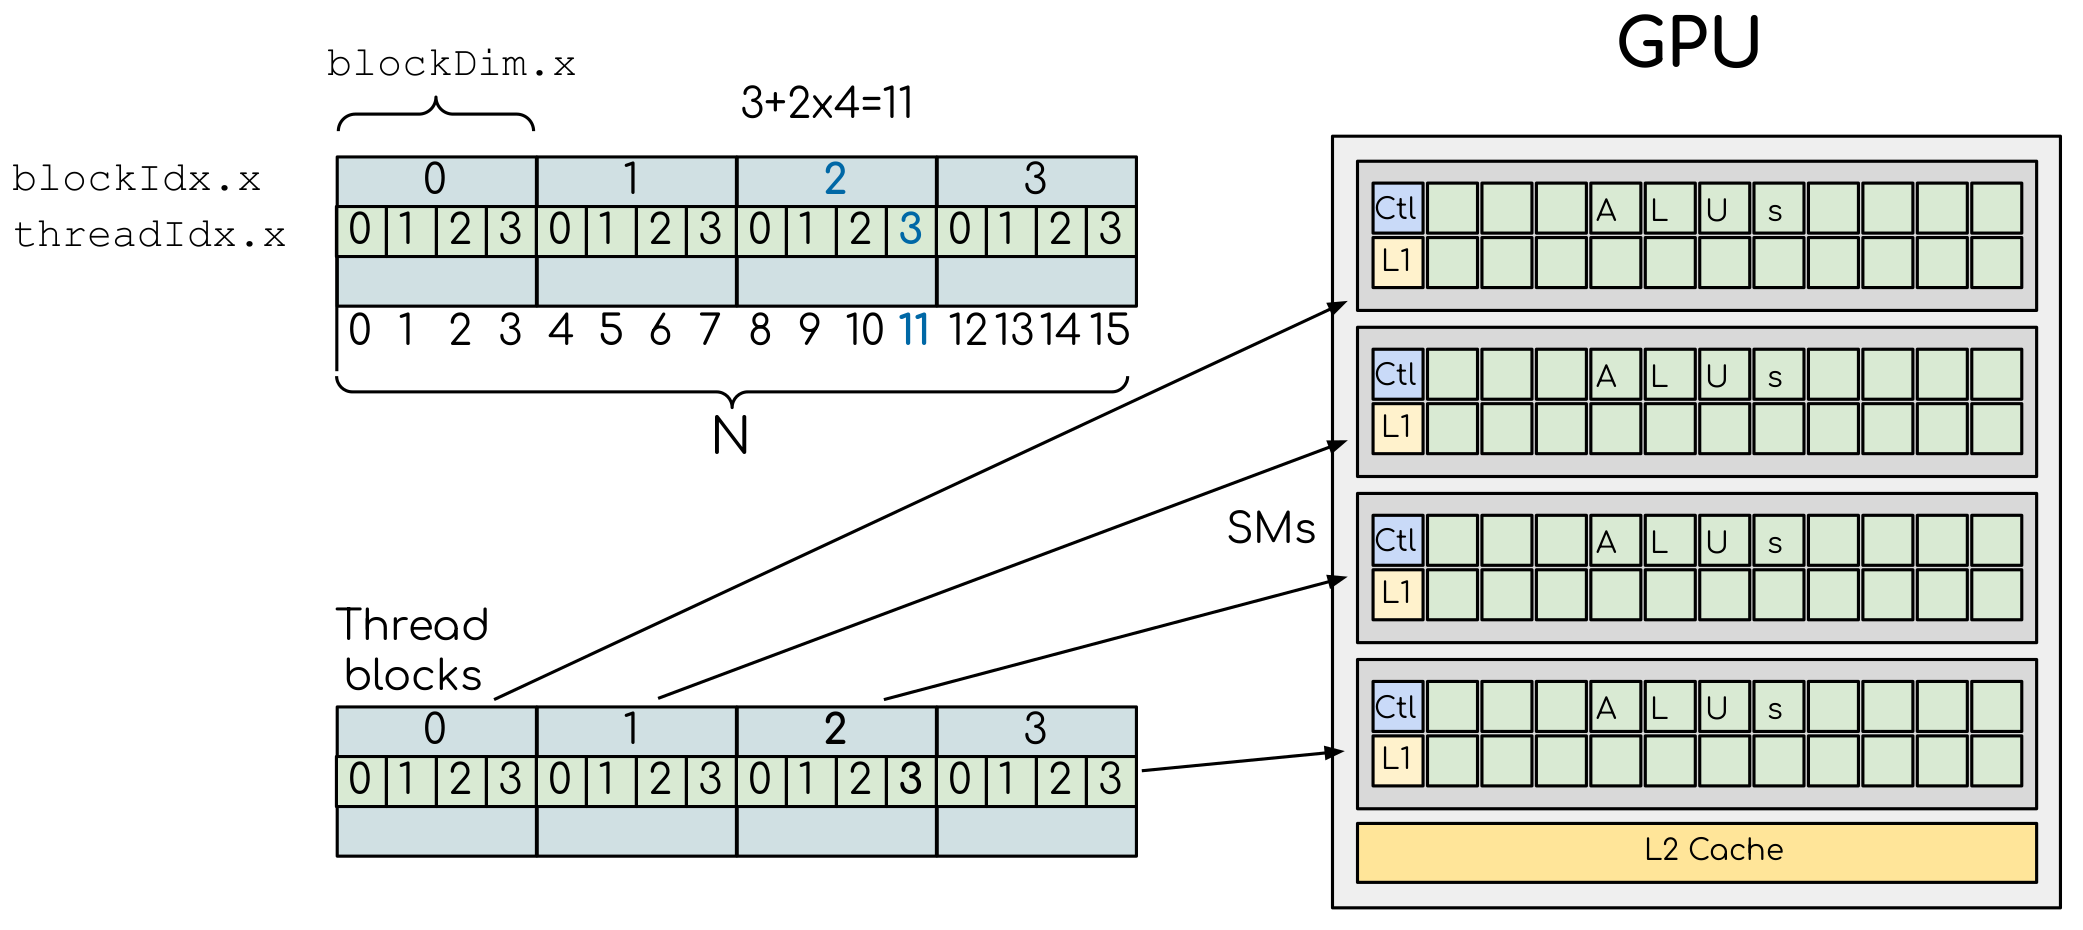
\includegraphics[width=0.8\textwidth]{fig_hardware/mapping_blocks_2_SMs.png}
\caption{Mapping thread and thread block indexes to SMPs on GPU.}\label{fig:mapping_blocks_2_SMs}
\end{figure}


\par
Below is an example of vector addition kernel for NVIDIA (List~\ref{lst:06_julia_own_kernel_nvidia}), AMD (List~\ref{lst:06_julia_own_kernel_amd}), Intel (List~\ref{lst:06_julia_own_kernel_intel}) and Apple (List~\ref{lst:06_julia_own_kernel_apple}) GPUs.


\lstinputlisting[language=python, caption={The vector addition kernel for NVIDIA GPU.}, label={lst:06_julia_own_kernel_nvidia}, xleftmargin=0.05\textwidth, xrightmargin=0.05\textwidth]{code_examples/06_julia_own_kernel_nvidia.jl}


\lstinputlisting[language=python, caption={The vector addition kernel for AMD GPU.}, label={lst:06_julia_own_kernel_amd}, xleftmargin=0.05\textwidth, xrightmargin=0.05\textwidth]{code_examples/06_julia_own_kernel_amd.jl}


\lstinputlisting[language=python, caption={The vector addition kernel for Intel GPU.}, label={lst:06_julia_own_kernel_intel}, xleftmargin=0.05\textwidth, xrightmargin=0.05\textwidth]{code_examples/06_julia_own_kernel_intel.jl}


\lstinputlisting[language=python, caption={The vector addition kernel for Apple GPU.}, label={lst:06_julia_own_kernel_apple}, xleftmargin=0.05\textwidth, xrightmargin=0.05\textwidth]{code_examples/06_julia_own_kernel_apple.jl}


\par
Two additional points should be address here.
\begin{itemize}
    \item \textbf{Restrictions in kernel programming}: Within kernels, most of the Julia language is supported with the exception of functionality that requires the Julia runtime library. This means one cannot allocate memory or perform dynamic function calls, both of which are easy to do accidentally!
    \item \textbf{1D, 2D and 3D}:~\textbf{\textcolor{brown}{CUDA.jl}} and~\textbf{\textcolor{brown}{AMDGPU.jl}} support indexing in up to 3 dimensions ($x$, $y$ and $z$, $e.g.$, $threadIdx().x$ and $workitemIdx().x$). This is convenient for multidimensional data where thread blocks can be organised into 1D, 2D or 3D arrays of threads.
\end{itemize}


\par
More reading materials related to the topics discussed above are available at:
\begin{itemize}
    \item~\href{https://enccs.github.io/hpda-python/parallel-computing/}{Python for HPDA} (ENCCS)
    \item~\href{https://uppmax.github.io/HPC-python/}{Python in HPC} (UPPMAX-HPC2N)
    \item~\href{https://enccs.github.io/julia-for-hpc/}{Julia for HPC}
\end{itemize}


\section{Directive-Based Programming Models}\label{sec:directive-based-programming-models}


\par
The most common directive-based models for GPU parallel programming are OpenACC and OpenMP offloading approaches.
The parallelization is done by introducing directives in places which are targeted for parallelization.
\begin{itemize}
    \item OpenACC is known to be more~\textbf{descriptive}, which means the programmer uses directives to tell the compiler how/where to parallelize the code and to move the data.
    \item OpenMP offloading approach, on the other hand, is known to be more~\textbf{prescriptive}, where the programmer uses directives to tell the compiler more explicitly how/where to parallelize the code, instead of letting the compiler decides.
\end{itemize}


\par
In OpenMP/OpenACC, the compiler directives are specified by using~\textbf{\textcolor{red}{\#pragma}} in C/C++ or as special comments identified by unique sentinels in Fortran.
Compilers can ignore the directives if the support for OpenMP/OpenACC is not enabled.
The compiler directives are used for various purposes: for thread creation, workload distribution (work sharing), data-environment management, serializing sections of code or for synchronization of work among the threads.


% -------------------------------------------------------------------- %


\subsection{Execution model}


\par
OpenMP and OpenACC use the fork-join model (Fig.~\ref{fig:fork_join}) of parallel execution.
The program begins as a single thread of execution, the master thread, which executes sequentially until the first parallel region construct is encountered.
When a parallel region is encountered, the master thread creates a group of threads, becomes the master of this group of threads, and is assigned the thread index 0 within the group (the green blocks in parallel regions in Fig.~\ref{fig:fork_join}).
There is an implicit barrier at the end of the parallel regions.
When the group of threads complete the statements in the parallel region construct, they synchronize and terminate, leaving only the master thread.
It is noted that the number of parallel regions and the threads that comprise them are arbitrary.


\begin{figure}[!htbp]
\centering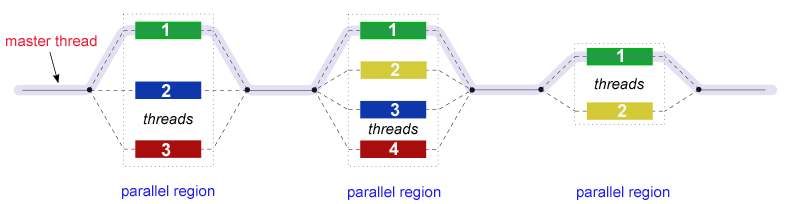
\includegraphics[width=0.8\textwidth]{fig_hardware/fork_join_model.png}
\caption{The fork-join model for parallel execution.}\label{fig:fork_join}
\end{figure}


% -------------------------------------------------------------------- %


\subsection{Offloading directives}


\subsubsection{OpenACC}


\par
In OpenACC, one of the most commonly used directives is~\textbf{\textcolor{red}{kernels}}, which defines a region to be transferred into a series of kernels to be executed in sequence on a GPU.
Work sharing is defined automatically for the separate kernels, but tuning prospects is limited.
Herein we provide code examples for OpenACC kernels in C++ and Fortran in List~\ref{lst:07_openacc_kernel_cpp} and List~\ref{lst:07_openacc_kernel_fortran}, respectively.


\lstinputlisting[language=c++, caption={Code example for OpenACC~\textbf{\textcolor{red}{kernels}} in C++. The 17$^{th}$ line indicates the starting point of OpenACC~\textbf{\textcolor{red}{kernels}}.}, label={lst:07_openacc_kernel_cpp}, xleftmargin=0.05\textwidth, xrightmargin=0.05\textwidth]{code_examples/07_openacc_kernel_cpp.cpp}


\lstinputlisting[language=fortran, caption={Code example for OpenACC~\textbf{\textcolor{red}{kernels}} in Fortran. The 14$^{th}$ and 18$^{th}$ lines indicate the starting and ending of the OpenACC~\textbf{\textcolor{red}{kernels}}.}, label={lst:07_openacc_kernel_fortran}, xleftmargin=0.05\textwidth, xrightmargin=0.05\textwidth]{code_examples/07_openacc_kernel_fortran.f}


\par
The other approach of OpenACC to define parallel regions is to use~\textbf{\textcolor{red}{parallel}} directive.
Contrary to the~\textbf{\textcolor{red}{kernels}} directive, the~\textbf{\textcolor{red}{parallel}} directive is more explicit and requires more analysis by the programmer.
Work sharing has to be defined manually using the~\textbf{\textcolor{red}{loop}} directive, and refined tuning is possible to achieve.
The code examples shown in List~\ref{lst:07_openacc_kernel_cpp} and List~\ref{lst:07_openacc_kernel_fortran} can be rewritten using the~\textbf{\textcolor{red}{parallel loop}}, as shown in List~\ref{lst:07_openacc_parallel_loop_cpp} and List~\ref{lst:07_openacc_parallel_loop_fortran}, respectively.


\lstinputlisting[language=c++, caption={Code example for OpenACC~\textbf{\textcolor{red}{parallel loop}} in C++. The 17$^{th}$ line indicates the starting point of OpenACC~\textbf{\textcolor{red}{parallel loop}}.}, label={lst:07_openacc_parallel_loop_cpp}, xleftmargin=0.05\textwidth, xrightmargin=0.05\textwidth]{code_examples/07_openacc_parallel_loop_cpp.cpp}


\lstinputlisting[language=fortran, caption={Code example for OpenACC~\textbf{\textcolor{red}{parallel loop}} in Fortran. The 14$^{th}$ and 18$^{th}$ lines indicate the starting and ending of the OpenACC~\textbf{\textcolor{red}{parallel loop}}.}, label={lst:07_openacc_parallel_loop_fortran}, xleftmargin=0.05\textwidth, xrightmargin=0.05\textwidth]{code_examples/07_openacc_parallel_loop_fortran.f}


\par
Sometimes we can obtain a little more performance by guiding the compiler to make specific choices.
OpenACC has four levels of parallelism for offloading execution:
\begin{itemize}
    \item \textbf{gang} coarse grain: the iterations are distributed among the gangs
    \item \textbf{worker} fine grain: worker’s threads are activated within gangs and iterations are shared among the threads
    \item \textbf{vector}: each worker activates its threads working in SIMT fashion and the work is shared among the threads
    \item \textbf{seq}: the iterations are executed sequentially
\end{itemize}


\par
It should be noted that:
\begin{itemize}
    \item By default,~\textbf{gang},~\textbf{worker} and~\textbf{vector} parallelism are automatically decided and applied by the compiler.
    \item The programmer could add clauses like~\textbf{\textcolor{red}{num\_gangs}},~\textbf{\textcolor{red}{num\_workers}} and~\textbf{\textcolor{red}{vector\_length}} within the parallel region to specify the number of gangs, workers and vector length.
    \item The optimal numbers are highly GPU architecture and compiler implementation dependent though.
    \item There is no thread synchronization at~\textbf{gang} level, which means there maybe a risk of race condition.
\end{itemize}


\subsubsection{OpenMP}


\par
With OpenMP, the~\textbf{\textcolor{red}{target}} directive is used for device offloading.
List~\ref{lst:07_openmp_target_construct_cpp} and List~\ref{lst:07_openmp_target_construct_fortran} provide code examples for OpenMP~\textbf{\textcolor{red}{target}} construct in C++ and Fortran, respectively.


\lstinputlisting[language=c++, caption={Code example for OpenMP~\textbf{\textcolor{red}{target}} construct in C++. The 16$^{th}$ line indicates the starting point of OpenMP~\textbf{\textcolor{red}{target}} construct.}, label={lst:07_openmp_target_construct_cpp}, xleftmargin=0.05\textwidth, xrightmargin=0.05\textwidth]{code_examples/07_openmp_target_construct.cpp}


\lstinputlisting[language=fortran, caption={Code example for OpenMP~\textbf{\textcolor{red}{target}} construct in Fortran. The 14$^{th}$ and 18$^{th}$ lines indicate the starting and ending of OpenMP~\textbf{\textcolor{red}{target}} construct.}, label={lst:07_openmp_target_construct_fortran}, xleftmargin=0.05\textwidth, xrightmargin=0.05\textwidth]{code_examples/07_openmp_target_construct.f}


\par
Compared to the OpenACC’s~\textbf{\textcolor{red}{kernels}} directive, the OpenMP's~\textbf{\textcolor{red}{target}} directive will not parallelise the underlying loop at all.
To achieve proper parallelisation, one needs to be more prescriptive and specify what one wants.
OpenMP offloading offers multiple levels of parallelism as well:
\begin{itemize}
    \item \textbf{teams} coarse grain: creates a league of teams and one master thread in each team, but no worksharing among the teams
    \item \textbf{distribute} distributes the iterations across the master threads in the teams, but no worksharing among the threads within one team
    \item \textbf{parallel do/for} fine grain: threads are activated within one team and worksharing among them
    \item \textbf{SIMD} like the~\textbf{vector} directive in OpenACC.
\end{itemize}


\par
It should be noted that:
\begin{itemize}
    \item The programmer could add clauses like~\textbf{\textcolor{red}{num\_teams}} and~\textbf{\textcolor{red}{thread\_limit}} to specify the number of teams and threads within a team.
    \item Threads in a team can synchronize but no synchronization among the teams.
    \item Since OpenMP 5.0, there is a new~\textbf{\textcolor{red}{loop}} directive available, which has the similar functionality as the corresponding one in OpenACC.
\end{itemize}


\par
Table~\ref{tbl:openacc_openmp_directive} provides a general mapping between OpenACC/OpenMP directives and GPU (HPE implementation).


\begin{table}
\centering\caption{Mapping between OpenACC/OpenMP directives and GPU (HPE implementation).}\label{tbl:openacc_openmp_directive}
\begin{tabular}{ |c|c|c|c| } 
\hline
\textbf{NVIDIA} & \textbf{AMD} & \textbf{Fortran OpenACC/OpenMP} & \textbf{C/C++ OpenMP} \\
\hline
thread block & work group & gang/teams & teams \\ 
wrap & wavefront & worker/simd & parallel for simd \\
thread & work item & vector/simd & parallel for simd\\
\hline
\end{tabular}
\begin{tablenotes}
\footnotesize
% \begin{itemize}
    \item[a] Each compiler supports different levels of parallelism.
    \item[b] The size of~\textbf{gang}/\textbf{team}/\textbf{worker}/\textbf{vector\_length} can be chosen arbitrarily by the user but there are limits defined by the implementation.
    \item[c] The maximum thread/grid/block size can be found via~\textbf{rocminfo}/\textbf{nvaccelinfo}.
% \end{itemize}
\end{tablenotes}
\end{table}


\subsubsection{Levels of parallelism}


\par
In this exercise we would like to change the levels of parallelism using clauses.
First compile and run one of the example to find out the default number of block and thread set by compiler at runtime.
To make a change, adding clauses like~\textbf{\textcolor{red}{num\_gangs}},~\textbf{\textcolor{red}{num\_workers}},~\textbf{\textcolor{red}{vector\_length}} for OpenACC, and~\textbf{\textcolor{red}{num\_teams}} and~\textbf{\textcolor{red}{thread\_limit}} for OpenMP offloading.
Remember to set the environment by executing~\textbf{\textcolor{brown}{export CRAY\_ACC\_DEBUG=2}} at runtime.
List~\ref{lst:07_module_lumi_cpp} and List~\ref{lst:07_module_lumi_fortran} provide commands to compile and run the code examples interactively using the AMD GPU on LUMI-G HPC cluster.


\lstinputlisting[language=bash, firstline=4, lastline=16, caption={Modules and commands to compile and run C++ code example using AMD GPU on LUMI-G HPC cluster.}, label={lst:07_module_lumi_cpp}, xleftmargin=0.05\textwidth, xrightmargin=0.05\textwidth]{code_examples/07_module_lumi.pbs}


\lstinputlisting[language=bash, firstline=27, lastline=40, caption={Modules and commands to compile and run Fortran code example using AMD GPU on LUMI-G HPC cluster.}, label={lst:07_module_lumi_fortran}, xleftmargin=0.05\textwidth, xrightmargin=0.05\textwidth]{code_examples/07_module_lumi.pbs}


% -------------------------------------------------------------------------------- %


\subsection{Data Movement}

\par
Due to distinct memory spaces on host and device, transferring data becomes inevitable.
New directives are needed to specify how variables are transferred from the host to the device data environment.
The common transferred items consist of arrays (array sections), scalars, pointers, and structure elements.
Various data clauses used for data movement is summarised in Table~\ref{tbl:data_clauses_openacc_openmp}.

\begin{table}[!h]
\centering\caption{Data clauses using OpenACC and OpenMP for data movement.}\label{tbl:data_clauses_openacc_openmp}
\begin{tabular}{ | p{0.14\textwidth} | p{0.18\textwidth} | p{0.58\textwidth} | } 
\hline
\textbf{OpenACC} & \textbf{OpenMP} & \\
\hline
\textbf{copyin(list)} & \textbf{map(to:list)} & On entering the region, variables in the list are initialized on the device using the original values from the host\\
\textbf{copyout(list)} & \textbf{map(from:list)} & At the end of the target region, the values from variables in the list are copied into the original variables on the host. On entering the region, the initial value of the variables on the device is not initialized \\
\textbf{copy(list)} & \textbf{map(tofrom:list)} & The effect of both a map-to and a map-from \\
\textbf{create(list)} & \textbf{map(alloc:list)} & On entering the region, data is allocated and uninitialized on the device \\
\textbf{delete(list)} & \textbf{map(delete:list)} & Delete data on the device \\
\hline
\end{tabular}
\end{table}


\par
It is noted that one should be careful about the array section notation when mapping data arrays or pointers.
\begin{itemize}
    \item In C/C++: array[lower-bound:length]. The notation :N is equivalent to 0:N.
    \item In Fortran: array[lower-bound:upper-bound]. The notation :N is equivalent to 1:N.
\end{itemize}


\subsubsection{Data region}


\par
The specific data clause combined with the data directive constitutes the start of a data region.
How the directives create storage, transfer data, and remove storage on the device are classified as two categories:~\textbf{structured data region} and~\textbf{unstructured data region}.


\paragraph{Structured Data Region.}
A~\textbf{structured data region} is convenient for providing persistent data on the device which could be used for subsequent GPU directives.
Below we provide syntax for structured data region using OpenACC (List~\ref{lst:07_structured_data_region_acc_c} for C and List~\ref{lst:07_structured_data_region_acc_f} for Fortran) and OpenMP (List~\ref{lst:07_structured_data_region_mp_c} for C and List~\ref{lst:07_structured_data_region_mp_f} for Fortran).


\lstinputlisting[language=c++, firstline=4, lastline=5, caption={Syntax for structured data region using OpenACC C++.}, label={lst:07_structured_data_region_acc_c}, xleftmargin=0.05\textwidth, xrightmargin=0.05\textwidth]{code_examples/07_structured_data_region.cpp}


\lstinputlisting[language=fortran, firstline=4, lastline=6, caption={Syntax for structured data region using OpenACC Fortran.}, label={lst:07_structured_data_region_acc_f}, xleftmargin=0.05\textwidth, xrightmargin=0.05\textwidth]{code_examples/07_structured_data_region.f}


\lstinputlisting[language=c++, firstline=14, lastline=15, caption={Syntax for structured data region using OpenMP C++.}, label={lst:07_structured_data_region_mp_c}, xleftmargin=0.05\textwidth, xrightmargin=0.05\textwidth]{code_examples/07_structured_data_region.cpp}


\lstinputlisting[language=fortran, firstline=15, lastline=17, caption={Syntax for structured data region using OpenMP Fortran.}, label={lst:07_structured_data_region_mp_f}, xleftmargin=0.05\textwidth, xrightmargin=0.05\textwidth]{code_examples/07_structured_data_region.f}


\paragraph{Unstructured Data Region}
However it is inconvenient in real applications to use structured data region, therefore the~\textbf{unstructured data region} with much more freedom in creating and deleting of data on the device at any appropriate point is adopted.
Below we also provide syntax for structured data region using OpenACC (List~\ref{lst:07_unstructured_data_region_acc_c} for C and List~\ref{lst:07_unstructured_data_region_acc_f} for Fortran) and OpenMP (List~\ref{lst:07_unstructured_data_region_mp_c} for C and List~\ref{lst:07_unstructured_data_region_mp_f} for Fortran).


\lstinputlisting[language=c++, firstline=4, lastline=6, caption={Syntax for unstructured data region using OpenACC C++.}, label={lst:07_unstructured_data_region_acc_c}, xleftmargin=0.05\textwidth, xrightmargin=0.05\textwidth]{code_examples/07_unstructured_data_region.cpp}


\lstinputlisting[language=fortran, firstline=4, lastline=6, caption={Syntax for unstructured data region using OpenACC Fortran.}, label={lst:07_unstructured_data_region_acc_f}, xleftmargin=0.05\textwidth, xrightmargin=0.05\textwidth]{code_examples/07_unstructured_data_region.f}


\lstinputlisting[language=c++, firstline=15, lastline=17, caption={Syntax for unstructured data region using OpenMP C++.}, label={lst:07_unstructured_data_region_mp_c}, xleftmargin=0.05\textwidth, xrightmargin=0.05\textwidth]{code_examples/07_unstructured_data_region.cpp}


\lstinputlisting[language=fortran, firstline=15, lastline=17, caption={Syntax for unstructured data region using OpenMP Fortran.}, label={lst:07_unstructured_data_region_mp_f}, xleftmargin=0.05\textwidth, xrightmargin=0.05\textwidth]{code_examples/07_unstructured_data_region.f}


\par
The keypoints for structured and unstructured data region are summarized below.
\begin{itemize}
    \item \textbf{Structured Data Region}
    \begin{itemize}
        \item Start and end points within a single subroutine
        \item Memory exists within the data region
    \end{itemize}
    \item \textbf{Unstructured Data Region}
    \begin{itemize}
        \item Multiple start and end points across different subroutines
        \item Memory exists until explicitly deallocated
    \end{itemize}
\end{itemize}


\paragraph{Update}
Sometimes, variables need to be synchronized between the host and the device memory, $e.g.$, in order to write out variables on the host for debugging or visualization, and it is often used in conjunction with unstructured data regions.
To control data transfer direction, a motion-clause must be present.
Below we also provide syntax for the~\textbf{\textcolor{red}{update}} directive using OpenACC (List~\ref{lst:07_update_directive_acc_c} for C and List~\ref{lst:07_update_directive_acc_f} for Fortran) and OpenMP (List~\ref{lst:07_update_directive_mp_c} for C and List~\ref{lst:07_update_directive_mp_f} for Fortran).


\lstinputlisting[language=c++, firstline=4, lastline=8, caption={Syntax for the~\textbf{\textcolor{red}{update}} directive using OpenACC C++.}, label={lst:07_update_directive_acc_c}, xleftmargin=0.05\textwidth, xrightmargin=0.05\textwidth]{code_examples/07_update_directive.cpp}


\lstinputlisting[language=fortran, firstline=4, lastline=8, caption={Syntax for the~\textbf{\textcolor{red}{update}} directive using OpenACC Fortran.}, label={lst:07_update_directive_acc_f}, xleftmargin=0.05\textwidth, xrightmargin=0.05\textwidth]{code_examples/07_update_directive.f}


\lstinputlisting[language=c++, firstline=15, lastline=19, caption={Syntax for the~\textbf{\textcolor{red}{update}} directive using OpenMP C++.}, label={lst:07_update_directive_mp_c}, xleftmargin=0.05\textwidth, xrightmargin=0.05\textwidth]{code_examples/07_update_directive.cpp}


\lstinputlisting[language=fortran, firstline=17, lastline=21, caption={Syntax for the~\textbf{\textcolor{red}{update}} directive using OpenMP Fortran.}, label={lst:07_update_directive_mp_f}, xleftmargin=0.05\textwidth, xrightmargin=0.05\textwidth]{code_examples/07_update_directive.f}


\par
It should be noted that the~\textbf{\textcolor{red}{update}} directive can only be used in host code since data movement must be initiated from the host, $i.e.$, it may not appear inside of a compute region.
In addition, motion-clause~\lq\lq host\rq\rq~has been deprecated and renamed~\lq\lq self\rq\rq~in OpenACC.


\par
Herein, we provide exercises (List~\ref{lst:07_update_mp_c} for OpenMP C++ and List~\ref{lst:07_update_acc_f} for OpenACC Fortran) for the~\textbf{update} directive to figure out the variable values on host and device at each check point, and the results for these exercises are provided at Table~\ref{tbl:solution_update_directive}.


\lstinputlisting[language=c++, caption={Code example for the~\textbf{\textcolor{red}{update}} directive using OpenMP C++.}, label={lst:07_update_mp_c}, xleftmargin=0.05\textwidth, xrightmargin=0.05\textwidth]{code_examples/07_update.cpp}


\lstinputlisting[language=fortran, caption={Code example for the~\textbf{\textcolor{red}{update}} directive using OpenACC Fortran.}, label={lst:07_update_acc_f}, xleftmargin=0.05\textwidth, xrightmargin=0.05\textwidth]{code_examples/07_update.f}


\begin{table}[!h]
\centering\caption{Computational results for the~\textbf{update} directive examples in List~\ref{lst:07_update_mp_c} for OpenMP C++ and List~\ref{lst:07_update_acc_f} for OpenACC Fortran.}\label{tbl:solution_update_directive}
\begin{tabular}{ |  c  |  c  |  c  | } 
\hline
check point & x on host & x on device \\
\hline
check point1 & 0 & 0 \\
check point2 & 10 & 0 \\
check point3 & 10 & 10 \\
\hline
\end{tabular}
\end{table}


\par
In addition, code examples of a vector addition problem using OpenACC/OpenMP for C++ and Fortran are provided here in the subdirectory of this repository~\cite{gpu-programming-examples}

\textbf{\textcolor{brown}{content/examples/exercise/07\_vec\_add/07\_vector\_addition\_acc.cpp}}

\textbf{\textcolor{brown}{content/examples/exercise/07\_vec\_add/07\_vector\_addition\_acc.f}}

\textbf{\textcolor{brown}{content/examples/exercise/07\_vec\_add/07\_vector\_addition\_omp.cpp}}

\textbf{\textcolor{brown}{content/examples/exercise/07\_vec\_add/07\_vector\_addition\_omp.f}}




\subsubsection{Optimize Data Transfer}


\par
There are several points that should be mentioned to optimize data transfer.
\begin{itemize}
    \item Explicitly transfer the data as much as possible.
    \item Reduce the amount of data mapping between host and device, get rid of unnecessary data transfer.
    \item Try to keep data environment residing on the device as long as possible.
\end{itemize}


% -------------------------------------------------------------------- %


\subsection{Pros of directive-based frameworks}


\par
Here are several advantages for the directive-based models for GPU parallel programming using OpenACC and OpenMP offloading.
\begin{itemize}
    \item Incremental programming
    \item Porting of existing software requires less work
    \item Same code can be compiled to CPU and GPU versions easily using compiler flag
    \item Low learning curve, do not need to know low-level hardware details
    \item Good portability
\end{itemize}


\par
The keypoints for the OpenACC and OpenMP offloading are summarized as follows:
\begin{itemize}
    \item OpenACC and OpenMP offloading enables you to annotate your code with special directives to identify areas to be executed in parallel on a GPU.
    \item This saves time compared to lower-level approaches, but you need to be mindful of memory movement.
\end{itemize}


\par
More materials for the OpenACC and OpenMP offloading models are provided in our previous training materials at
\begin{itemize}
    \item~\href{https://enccs.github.io/openacc/}{ENCCS lesson on OpenACC}
    \item~\href{https://enccs.github.io/openmp-gpu/}{ENCCS lesson on OpenMP for GPU offloading}.
\end{itemize}


\section{Multiple GPU Programming with MPI}


\subsection{Introduction}


\par
Exploring multiple GPUs across distributed nodes offers the potential to fully leveraging the capacity of modern HPC systems at a large scale.
One of the approaches to accelerate computing on distributed systems is to combine MPI (Message Passing Interface) with a GPU programming model such as OpenACC and OpenMP.
This combination is motivated by both the simplicity of these APIs, and the widespread use of MPI.


\par
In this guide we provide readers with insighits on implementing a hybrid model in which the MPI communication framework is combined with either OpenACC or OpenMP APIs.
A special focus will be on performing point-to-point ($e.g.$,~\textbf{\textcolor{red}{MPI\_Send()}} and~\textbf{\textcolor{red}{MPI\_Recv()}}) and collective operations ($e.g.$~\textbf{\textcolor{red}{MPI\_Allreduce()}}) from OpenACC and OpenMP APIs.
Herein we address two scenarios: (i) a scenario in which MPI operations are performed in the CPU-host followed by an offload to the GPU-device; and (ii) a scenario in which MPI operations are performed between a pair of GPUs without involving the CPU-host memory.
The latter scenario is referred to as~\textbf{GPU-awareness MPI}, and has the advantage of reducing the computing time caused by transferring data $via$ the host-memory during heterogeneous communications, thus rendering HPC applications efficient.


\par
This guide in this section is organized as follows: we first introduce how to assign each MPI rank to a GPU device within the same node.
We consider a situation in which the host and device have a distinct memory.
This is followed by a presentation on the hybrid MPI-OpenACC/OpenMP offloading with and without the GPU-awareness MPI.
Exercises to help understanding these concepts are provided at the end of this section.


% -------------------------------------------------------------------- %


\subsection{Assigning MPI-ranks to GPU-devices}


\par
Accelerating MPI applications to utilise multiple GPUs on distributed nodes requires as a first step assigning each MPI rank to a GPU device, such that two MPI ranks do not use the same GPU device.
This is necessarily in order to prevent the application from a potential crash because GPUs are designed to handle multiple threading tasks, but not multiple MPI ranks.


\par
One way to ensure that two MPI ranks do not use the same GPU is to determine which MPI processes run on the same node, such that each process can be assigned to a GPU device within the same node.
This can be done, for instance, by splitting the world communicator into sub-groups of communicators (or sub-communicators) using the routine~\textbf{\textcolor{red}{MPI\_COMM\_SPLIT\_TYPE()}} shown in List~\ref{lst:08_split_communicator_mpi}. 


\lstinputlisting[language=fortran, caption={Splitting the world communicator into sub-groups of communicators in MPI.}, label={lst:08_split_communicator_mpi}, xleftmargin=0.05\textwidth, xrightmargin=0.05\textwidth]{code_examples/08_split_communicator_mpi.f}


\par
Herein, the size of each sub-communicator corresponds to the number of GPUs per node (which is also the number of tasks per node), and each sub-communicator contains a list of processes indicated by a rank.
These processes have a shared-memory region defined by the argument~\textbf{\textcolor{red}{MPI\_COMM\_TYPE\_SHARED()}} (see the~\href{https://www.mpi-forum.org/docs/mpi-4.0/mpi40-report.pdf}{MPI report} for more details).
Calling the routine~\textbf{\textcolor{red}{MPI\_COMM\_SPLIT\_TYPE()}} returns a sub-communicator labelled as $host\_comm$ in List~\ref{lst:08_split_communicator_mpi}, and in which MPI-ranks are ranked from 0 to the number of processes per node -1.
These MPI ranks are in turn assigned to different GPU devices within the same node.
This procedure is done according to which directive-based model is implemented.
The retrieved MPI ranks are then stored in the variable $myDevice$.
The variable is passed to an OpenACC and OpenMP routine as indicated in the code examples in List~\ref{lst:08_assign_set_device_acc} and List~\ref{lst:08_assign_set_device_omp}, respectively.


\lstinputlisting[language=fortran, firstline=4, caption={Assigning MPI ranks to different GPU devices and thereafter passing MPI ranks stored in the variable $myDevice$ to an OpenACC routine.}, label={lst:08_assign_set_device_acc}, xleftmargin=0.05\textwidth, xrightmargin=0.05\textwidth]{code_examples/08_assign_set_device_acc.f}


\lstinputlisting[language=fortran, firstline=4, caption={Assigning MPI ranks to different GPU devices and thereafter passing MPI ranks stored in the variable $myDevice$ to an OpenMP routine.}, label={lst:08_assign_set_device_omp}, xleftmargin=0.05\textwidth, xrightmargin=0.05\textwidth]{code_examples/08_assign_set_device_omp.f}


% ---------------------------------------------------------------------- %


\subsection{Hybrid MPI-OpenACC/OpenMP without GPU-awareness approach}


\par
After covering how to assign each MPI-rank to a GPU device, we now address the concept of combining MPI with either OpenACC or OpenMP offloading.
In this approach, calling an MPI routine from an OpenACC or OpenMP API requires updating the data in the CPU host before and after an MPI call.
In this scenario, the data is copied back and forth between the host and device before and after each MPI call.
In the hybrid MPI-OpenACC model, the procedure is defined by specifying the directive~\textbf{\textcolor{red}{update host()}} for copying the data from the device to the host before an MPI call; and by the directive~\textbf{\textcolor{red}{update device()}} specified after an MPI call for copying the data back to the device.
In the hybrid MPI-OpenMP model, updating the data in the host can be done by specifying the OpenMP directives~\textbf{\textcolor{red}{update device() from()}} and~\textbf{\textcolor{red}{update device() to()}}, respectively, for copying the data from the device to the host and back to the device.


\par
To illustrate the concept of the hybrid MPI-OpenACC/OpenMP, List~\ref{lst:08_update_host_device_directive_acc} and List~\ref{lst:08_update_host_device_directive_omp} present code examples for an implementation and an update of host/device directives that involve the MPI functions~\textbf{\textcolor{red}{MPI\_Send()}} and~\textbf{\textcolor{red}{MPI\_Recv()}}.


\lstinputlisting[language=fortran, firstline=5, caption={Implementation of MPI functions and update of host/device directives combining MPI with OpenACC.}, label={lst:08_update_host_device_directive_acc}, xleftmargin=0.05\textwidth, xrightmargin=0.05\textwidth]{code_examples/08_update_host_device_directive_acc.f}


\lstinputlisting[language=fortran, firstline=5, caption={Implementation of MPI functions and update of host/device directives combining MPI with OpenMP.}, label={lst:08_update_host_device_directive_omp}, xleftmargin=0.05\textwidth, xrightmargin=0.05\textwidth]{code_examples/08_update_host_device_directive_omp.f}


\par
Despite the simplicity of implementing the hybrid MPI-OpenACC/OpenMP offloading, it suffers from a low performance caused by an explicit transfer of data between the host and the device before and after calling an MPI routine.
This constitutes a bottleneck in GPU programming.
To improve the performance affected by the host staging during the data transfer, one can implement the GPU-awareness MPI approach as described in the following subsection.


% ---------------------------------------------------------------------- %


\subsection{Hybrid MPI-OpenACC/OpenMP with GPU-awareness approach}


\par
The concept of the GPU-aware MPI enables an MPI library to directly access the GPU-device memory without necessarily using the CPU-host memory as an intermediate buffer~\cite{gpu_aware_mpi}.
This offers the benefit of transferring data from one GPU to another GPU without the involvement of the CPU-host memory.


\par
To be specific, in the GPU-awareness approach, the device pointers point to the data allocated in the GPU memory space (data should be present in the GPU device).
The pointers are passed as arguments to an MPI routine that is supported by the GPU memory.
As MPI routines can directly access GPU memory, it offers the possibility of communicating between pairs of GPUs without transferring data back to the host.


\par
In the hybrid MPI-OpenACC model, the concept is defined by combining the directive~\textbf{\textcolor{red}{host\_data}} together with the clause~\textbf{\textcolor{red}{use\_device(list\_array)}}.
This combination enables the access to the arrays listed in the clause~\textbf{\textcolor{red}{use\_device(list\_array)}} from the host~\cite{openacc_u_device}.
The list of arrays, which are already present in the GPU-device memory, are directly passed to an MPI routine without a need of a staging host-memory for copying the data.
Note that for initially copying data to GPU, we use unstructured data blocks characterized by the directives~\textbf{\textcolor{red}{enter data}} and~\textbf{\textcolor{red}{exit data}}.
The unstructured data has the advantage of allowing to allocate and deallocate arrays within a data region.


\par
To illustarte the concept of the GPU-awareness MPI, we show code examples that make use of point-to-point and collective operations and the implementation of MPI functions~\textbf{\textcolor{red}{MPI\_Send()}}, \textbf{\textcolor{red}{MPI\_Recv()}} and~\textbf{\textcolor{red}{MPI\_Allreduce()}} with OpenACC and OpenMP APIs, as shown in List~\ref{lst:08_gpu_awareness_acc} and List~\ref{lst:08_gpu_awareness_omp}, respectively.
In the first part of each code example from the 6$^{st}$ to the 15$^{th}$ line, the device pointer~\textbf{f} is passed to the MPI functions~\textbf{\textcolor{red}{MPI\_Send()}} and~\textbf{\textcolor{red}{MP\_Recv()}}.
In the second part of each code example from 31$^{st}$ to 35$^{th}$ line, the pointer~\textbf{SumToT} is passed to the MPI function~\textbf{\textcolor{red}{MPI\_Allreduce()}}.
Herein, the MPI operations~\textbf{\textcolor{red}{MPI\_Send()}} and~\textbf{\textcolor{red}{MPI\_Recv()}} as well as~\textbf{\textcolor{red}{MPI\_Allreduce()}} are performed between a pair of GPUs without passing through the CPU-host memory.
In addition, the implementation of MPI functions with OpenACC and OpenMP APIs is specifically designed to support GPU-aware MPI operations.


\lstinputlisting[language=fortran, caption={Usage of point-to-point and collective operations using GPU-awareness MPI with OpenACC.}, label={lst:08_gpu_awareness_acc}, xleftmargin=0.05\textwidth, xrightmargin=0.05\textwidth]{code_examples/08_gpu_awareness_acc.f}


\lstinputlisting[language=fortran, caption={Usage of point-to-point and collective operations using GPU-awareness MPI with OpenMP.}, label={lst:08_gpu_awareness_omp}, xleftmargin=0.05\textwidth, xrightmargin=0.05\textwidth]{code_examples/08_gpu_awareness_omp.f}


\par
The GPU-aware MPI with OpenACC and OpenMP APIs has the capability of directly communicating between a pair of GPUs within a single node.
However, performing the GPU-to-GPU communication across multiple nodes requires the the GPUDirect RDMA (Remote Direct Memory Access) technology~\cite{gpudirect-rdma}.
This technology can further improve performance by reducing latency.


% ---------------------------------------------------------------------- %


\subsection{Compilation process}


\par
The compilation process of the hybrid MPI-OpenACC and MPI-OpenMP offloading is described below.
This description is given for a Cray compiler of the wrapper~\textbf{ftn}.
On the LUMI-G cluster, the following modules shown in List~\ref{lst:08_module_compile_command_git} may be necessary before compiling (see~\href{https://docs.lumi-supercomputer.eu/development/compiling/prgenv/}{LUMI documentation} for further details about the available programming environments).
The commands to compile code samples on LUMI-G cluster are also listed in List~\ref{lst:08_module_compile_command_git}.


\lstinputlisting[language=c++, firstline=4, lastline=14, caption={Modules and commands used to compile the code examples on the LUMI-G cluster.}, label={lst:08_module_compile_command_git}, xleftmargin=0.05\textwidth, xrightmargin=0.05\textwidth]{code_examples/08_module_compile_command_git.pbs}


\par
Here, the flags~\textbf{\textcolor{brown}{-hacc}} and~\textbf{\textcolor{brown}{-homp}} enable the OpenACC and OpenMP directives in the hybrid MPI-OpenACC and MPI-OpenMP applications, respectively.
In addition, to enable the GPU-aware support in MPICH library, one needs to set the following environment variable before running the application~\textbf{\textcolor{brown}{\$ export MPICH\_GPU\_SUPPORT\_ENABLED=1}}.


% ---------------------------------------------------------------------- %


\subsection{Exercises}


\par
We consider an MPI Fortran code that solves a 2D-Laplace equation, which is partially accelerated.
Code examples are available in the~\textbf{\textcolor{brown}{content/examples/exercise\_multipleGPU}} subdirectory of this repository~\cite{gpu-programming-examples}.
To access these code examples, you need to clone the repository via the commands:
\lstinputlisting[language=c++, firstline=21, lastline=22, xleftmargin=0.05\textwidth, xrightmargin=0.05\textwidth]{code_examples/08_module_compile_command_git.pbs}
The focus of this exercise is to complete the acceleration using either OpenACC or OpenMP API by following steps.


\begin{itemize}
    \item~\textbf{Exercise I}: Set a GPU device
    \begin{itemize}
        \item Implement OpenACC/OpenMP functions that enable assigning each MPI rank to a GPU device.
        \item Compile and run the code on multiple GPUs.
    \end{itemize}
    \item~\textbf{Exercise II}: Apply traditional MPI-OpenACC/OpenMP
    \begin{itemize}
        \item Incoporate the OpenACC directives~\textbf{\textcolor{red}{update host()}} and~\textbf{\textcolor{red}{update device()}} before and after calling an MPI function, respectively. (\textbf{Note}: The OpenACC directive~\textbf{\textcolor{red}{update host()}} is used to transfer data from GPU to CPU within a data region, while the directive~\textbf{\textcolor{red}{update device()}} is used to transfer the data from CPU to GPU.)
        \item Incorporate the OpenMP directives~\textbf{\textcolor{red}{update device() from()}} and~\textbf{\textcolor{red}{update device() to()}} before and after calling an MPI function, respectively. (\textbf{Note}: The OpenMP directive~\textbf{\textcolor{red}{update device() from()}} is used to transfer data from GPU to CPU within a data region, while the directive~\textbf{\textcolor{red}{update device() to()}} is used to transfer the data from CPU to GPU.)
        \item Compile and run the code on multiple GPUs.
    \end{itemize}
    \item~\textbf{Exercise III}: Implement GPU-aware support
    \begin{itemize}
        \item Incorporate the OpenACC directive~\textbf{\textcolor{red}{host\_data use\_device()}} to pass a device pointer to an MPI function.
        \item Incorporate the OpenMP directive~\textbf{\textcolor{red}{data use\_device\_ptr()}} to pass a device pointer to an MPI function.
        \item Compile and run the code on multiple GPUs.
    \end{itemize}
    \item~\textbf{Exercise IV}: Evaluate the performance
    \begin{itemize}
        \item Evaluate the execution time of the accelerated codes in the Exercises II and III, and compare it with that of a pure MPI implementation.
    \end{itemize}
\end{itemize}


% ---------------------------------------------------------------------- %


\subsection{Conclusion}


\par
In conclusion, we have presented an overview of a GPU-hybrid programming by integrating GPU-directive models, specifically OpenACC and OpenMP APIs, with the MPI library.
The approach adopted here allows us to utilise multiple GPU-devices not only within a single node but it extends to distributed nodes.
In particular, we have addressed GPU-aware MPI approach, which has the advantage of enabling a direct interaction between an MPI library and a GPU-device memory.
In other words, it permits performing MPI operations between a pair of GPUs, thus reducing the computing time caused by the data locality.


\par
More reading materials for MPI, OpenACC and OpenMP APIs are available at:
\begin{itemize}
    \item~\href{https://documentation.sigma2.no/code_development/guides/gpuaware_mpi.html}{GPU-aware MPI}
    \item~\href{https://www.mpi-forum.org/docs/mpi-4.0/mpi40-report.pdf}{MPI documentation}
    \item~\href{https://www.openacc.org/sites/default/files/inline-images/Specification/OpenACC-3.2-final.pdf}{OpenACC specification}
    \item~\href{https://www.openmp.org/wp-content/uploads/OpenMP-API-Specification-5-2.pdf}{OpenMP specification}
    \item~\href{https://docs.lumi-supercomputer.eu/development/compiling/prgenv/}{LUMI documentation}
    \item~\href{https://documentation.sigma2.no/code_development/guides/converting_acc2omp/openacc2openmp.html}{OpenACC vs OpenMP offloading}
    \item~\href{https://github.com/HichamAgueny/GPU-course}{OpenACC course}
\end{itemize}


\section{Non-Portable Kernel-Based Programming Models}\label{sec:non-portable-kernel-based-programming-models}


\subsection{Fundamentals of GPU programming with CUDA and HIP}


\par
Unlike some cross-platform portability ecosystems, such as Alpaka, Kokkos, OpenCL, RAJA, and SYCL, which cater to multiple architectures, CUDA and HIP are solely focused on GPUs.
They provide extensive libraries, APIs, and compiler toolchains that optimize code execution on NVIDIA GPUs (in the case of CUDA) and both NVIDIA and AMD GPUs (in the case of HIP).
Because they are developed by the device producers, these programming models provide high-performance computing capabilities and offer advanced features like shared memory, thread synchronization, and memory management specific to GPU architectures.


\par
CUDA, developed by NVIDIA, has gained significant popularity and is widely used for GPU programming.
It offers a comprehensive ecosystem that includes not only the CUDA programming model but also a vast collection of GPU-accelerated libraries.
Developers can write CUDA kernels using C++ and seamlessly integrate them into their applications to harness the massive parallelism of GPUs.


\par
HIP, on the other hand, is an open-source project that aims to provide a more~\lq\lq portable\rq\rq~GPU programming interface.
It allows developers to write GPU code in a syntax similar to CUDA and provides a translation layer that enables the same code to run on both NVIDIA and AMD GPUs.
This approach minimizes the effort required to port CUDA code to different GPU architectures and provides flexibility for developers to target multiple platforms.


\par
By being closely tied to the GPU hardware, CUDA and HIP provide a level of performance optimization that may not be achievable with cross-platform portability ecosystems.
The libraries and toolchains offered by these programming models are specifically designed to exploit the capabilities of the underlying GPU architectures, enabling developers to achieve high performance.


\par
Developers utilizing CUDA or HIP can tap into an extensive ecosystem of GPU-accelerated libraries, covering various domains, including linear algebra, signal processing, image processing, machine learning, and more.
These libraries are highly optimized to take advantage of the parallelism and computational power offered by GPUs, allowing developers to accelerate their applications without having to implement complex algorithms from scratch.


\par
As mentioned before, CUDA and HIP are very similar so it makes sense to cover both at the same time.
In the following parts, we will show three code samples of CUDA and HIP, and these code examples will be compared with those in the portable kernel-based frameworks of Kokkos, SYCL and OpenCL, which will be systematically discussed in the next section.


\subsubsection{Hello World}


\par
The~\lq\lq Hello World\rq\rq~example is the most basic ones for any programming language.
Herein we provide this example of CUDA (List~\ref{lst:09_hello_world_cuda}) and HIP (List~\ref{lst:09_hello_world_hip}), and also of portable kernel-based models of Kokkos (List~\ref{lst:09_hello_world_kokkos}), OpenCL (List~\ref{lst:09_hello_world_opencl}) and SYCL (List~\ref{lst:09_hello_world_sycl}).


\lstinputlisting[language=c++, firstline=4, lastline=17, caption={The~\lq\lq Hello World\rq\rq~example of CUDA.}, label={lst:09_hello_world_cuda}, xleftmargin=0.05\textwidth, xrightmargin=0.05\textwidth]{code_examples/09_hello_world.cpp}


\lstinputlisting[language=c++, firstline=26, lastline=38, caption={The~\lq\lq Hello World\rq\rq~example of HIP.}, label={lst:09_hello_world_hip}, xleftmargin=0.05\textwidth, xrightmargin=0.05\textwidth]{code_examples/09_hello_world.cpp}


\lstinputlisting[language=c++, firstline=47, lastline=62, caption={The~\lq\lq Hello World\rq\rq~example of Kokkos.}, label={lst:09_hello_world_kokkos}, xleftmargin=0.05\textwidth, xrightmargin=0.05\textwidth]{code_examples/09_hello_world.cpp}


\lstinputlisting[language=c++, firstline=71, lastline=89, caption={The~\lq\lq Hello World\rq\rq~example of OpenCL.}, label={lst:09_hello_world_opencl}, xleftmargin=0.05\textwidth, xrightmargin=0.05\textwidth]{code_examples/09_hello_world.cpp}


\lstinputlisting[language=c++, firstline=98, lastline=109, caption={The~\lq\lq Hello World\rq\rq~example of SYCL.}, label={lst:09_hello_world_sycl}, xleftmargin=0.05\textwidth, xrightmargin=0.05\textwidth]{code_examples/09_hello_world.cpp}


\par
In the code examples of CUDA and HIP, we include the necessary headers:~\textbf{\textcolor{brown}{cuda\_runtime.h}} and~\textbf{\textcolor{brown}{cuda.h}} for CUDA, and~\textbf{\textcolor{brown}{hip\_runtime.h}} for HIP.
These headers provide the required functionality for GPU programming.


\par
To retrieve information about the available devices, we use the functions~\textbf{\textcolor{red}{$<$cuda/hip$>$}} \textbf{\textcolor{red}{GetDeviceCount}} and~\textbf{\textcolor{red}{$<$cuda/hip$>$GetDevice}}.
These functions allow us to determine the total number of GPUs and the index of the currently used device.
In the code examples, we default to use device 0.


\subsubsection{Vector Addition}\label{sec:vector_addition}


\par
To demonstrate the fundamental features of CUDA/HIP programming, we begin with a straightforward task of element-wise vector addition.
The code examples below demonstrate how to utilize CUDA (List~\ref{lst:09_vector_addition_cuda}) and HIP (List~\ref{lst:09_vector_addition_hip}) for efficiently executing this operation.
In addition, the code samples of portable kernel-based models of OpenCL (List~\ref{lst:09_vector_addition_opencl}) and SYCL (List~\ref{lst:09_vector_addition_sycl}) are also provided for a comparative purpose.


\lstinputlisting[language=c++, caption={The~\lq\lq Vector Addition\rq\rq~example of CUDA.}, label={lst:09_vector_addition_cuda}, xleftmargin=0.05\textwidth, xrightmargin=0.05\textwidth]{code_examples/09_vector_addition_cuda.cpp}


\lstinputlisting[language=c++, caption={The~\lq\lq Vector Addition\rq\rq~example of HIP.}, label={lst:09_vector_addition_hip}, xleftmargin=0.05\textwidth, xrightmargin=0.05\textwidth]{code_examples/09_vector_addition_hip.cpp}


\lstinputlisting[language=c++, caption={The~\lq\lq Vector Addition\rq\rq~example of OpenCL.}, label={lst:09_vector_addition_opencl}, xleftmargin=0.05\textwidth, xrightmargin=0.05\textwidth]{code_examples/09_vector_addition_opencl.cpp}


\lstinputlisting[language=c++, caption={The~\lq\lq Vector Addition\rq\rq~example of SYCL.}, label={lst:09_vector_addition_sycl}, xleftmargin=0.05\textwidth, xrightmargin=0.05\textwidth]{code_examples/09_vector_addition_sycl.cpp}


\par
In this case, the CUDA and HIP codes are equivalent one to one so we will only refer to the CUDA version.
The CUDA and HIP programming model are host centric programming models.
The main program is executed on CPU and controls all the operations, memory allocations, data transfers between CPU and GPU, and launches the kernels to be executed on the GPU.
The code starts with defining the GPU kernel function called~\textbf{\textcolor{red}{vector\_add}} with attribute~\textbf{\textcolor{red}{\_\_global\_\_}}.
It takes three input arrays $A$, $B$, and $C$ along with the array size $n$.
The kernel function contains the actually code which is executed on the GPU by multiple threads in parallel.


\par
Accelerators in general and GPUs in particular have their own dedicated memory separate from the system memory (this could change soon! see latest info about~\textbf{AMD MI300}~\cite{amd_mi300} and~\textbf{NVIDIA Hopper}~\cite{nvidia_hopper}).
When programming for GPUs, there are two sets of pointers involved and it’s necessary to manage data movement between the host memory and the accelerator memory.
Data needs to be explicitly copied from the host memory to the accelerator memory before it can be processed by the accelerator.
Similarly, the obtained computational results or modified data may need to be copied back from the accelerator memory to the host memory to make them accessible to the CPU.


\par
The main function of the code initializes the input arrays $Ah$, $Bh$ on the CPU and computes the reference array $Cref$.
It then allocates memory on the GPU for the input and output arrays $Ad$, $Bd$, and $Cd$ using~\textbf{\textcolor{red}{cudaMalloc}} (herein, $h$ is for the host (CPU) and $d$ for the device (GPU)).
The data is transferred from the CPU to the GPU using~\textbf{\textcolor{red}{hipMemcpy}}, and then the GPU kernel is launched using the $<<<.>>>$ syntax.
All kernels launch are asynchronous.
After launch the control returns to the $main()$ and the code proceeds to the next instructions.


\par
After the kernel execution, the result array $Cd$ is copied back to the CPU using~\textbf{\textcolor{red}{cudaMemcpy}}.
The code then prints the reference and result arrays, calculates the error by comparing the reference and result arrays.
Finally, the GPU and CPU memory are deallocated using~\textbf{\textcolor{red}{cudaFree}} and~\textbf{\textcolor{red}{free}} functions, respectively.


\par
The host functions~\textbf{\textcolor{red}{cudaSetDevice}},~\textbf{\textcolor{red}{cudaMalloc}},~\textbf{\textcolor{red}{cudaMemcpy}}, and~\textbf{\textcolor{red}{cudaFree}} are blocking, $i.e.$, the code does not continues to next instructions until the operations are completed.
However this is not the default behaviour, for many operations there are asynchrounous equivalents and there are as well many library calls return the control to the $main()$ after calling. 
This allows the developers to launch independent operations and overlap them.


\par
In short, this code demonstrates how to utilize the CUDA and HIP to perform vector addition on a GPU, showcasing the steps involved in allocating memory, transferring data between the CPU and GPU, launching a kernel function, and handling the results.
It serves as a starting point for GPU-accelerated computations using CUDA and HIP.
More code examples for the~\lq\lq vector (array) addition\rq\rq~program are available in the~\textbf{\textcolor{brown}{content/examples/}} subdirectory of this repository~\cite{gpu-programming-examples}.


\par
In order to practice the concepts mentioned above, you can edit the skeleton code in the repository and the code corresponding to setting the device, memory allocations and transfers, and the kernel execution.


\subsubsection{Vector Addition with Unified Memory}


\par
For a while already GPUs support unified memory, which allows to use the same pointer for both CPU and GPU data.
This simplifies developing codes by removing the explicit data transfers.
The data resides on CPU until it is needed on GPU or vice-versa.
However the data transfers still happens~\lq\lq under the hood\rq\rq~and the developer needs to construct the code to avoid unnecessary transfers.
Below one can see the modified code examples (List~\ref{lst:09_vector_addition_with_unified_memory_cuda} for CUDA, List~\ref{lst:09_vector_addition_with_unified_memory_hip} for HIP, and List~\ref{lst:09_vector_addition_with_unified_memory_sycl} for SYCL) for the vector addition program using unified memory in GPU.


\lstinputlisting[language=c++, caption={The~\lq\lq Vector Addition with Unified Memory\rq\rq~example of CUDA.}, label={lst:09_vector_addition_with_unified_memory_cuda}, xleftmargin=0.05\textwidth, xrightmargin=0.05\textwidth]{code_examples/09_vector_addition_with_unified_memory_cuda.cpp}


\lstinputlisting[language=c++, caption={The~\lq\lq Vector Addition with Unified Memory\rq\rq~example of HIP.}, label={lst:09_vector_addition_with_unified_memory_hip}, xleftmargin=0.05\textwidth, xrightmargin=0.05\textwidth]{code_examples/09_vector_addition_with_unified_memory_hip.cpp}


\lstinputlisting[language=c++, caption={The~\lq\lq Vector Addition with Unified Memory\rq\rq~example of SYCL.}, label={lst:09_vector_addition_with_unified_memory_sycl}, xleftmargin=0.05\textwidth, xrightmargin=0.05\textwidth]{code_examples/09_vector_addition_with_unified_memory_sycl.cpp}


\par
It is shown that the arrays $Ah$, $Bh$, $Ch$, and $Cref$ are using~\textbf{\textcolor{red}{cudaMallocManaged}} to allocate unified memory in GPU.
The~\textbf{\textcolor{red}{vector\_add}} kernel is launched by passing these unified memory pointers directly.
After the kernel launch,~\textbf{\textcolor{red}{cudaDeviceSynchronize}} is used to wait for the kernel to complete execution.
Finally,~\textbf{\textcolor{red}{cudaFree}} is used to free the unified memory arrays.
The unified memory allows for transparent data migration between CPU and GPU, eliminating the need for explicit data transfers.


\par
A short summary of GPU programming with CUDA and HIP:
\begin{itemize}
    \item CUDA is developed by NVIDIA, while HIP is an open-source project (from AMD) for multi-platform GPU programming.
    \item CUDA and HIP are GPU-focused programming models for optimized code execution on NVIDIA and AMD GPUs.
    \item CUDA and HIP are similar, allowing developers to write GPU code in a syntax similar to CUDA and target multiple platforms.
    \item CUDA and HIP are programming models focused solely on GPUs
    \item CUDA and HIP offer high-performance computing capabilities and advanced features specific to GPU architectures, such as shared memory and memory management.
    \item They provide highly GPU-accelerated libraries in various domains like linear algebra, signal processing, image processing, and machine learning.
    \item Programming for GPUs involves managing data movement between host and accelerator memory.
    \item Unified memory simplifies data transfers by using the same pointer for CPU and GPU data, but code optimization is still necessary.
\end{itemize}


% ---------------------------------------------------------------------- %


\subsection{Memory Optimizations}\label{sec:memory_optimization}


\par
Vector addition is a relatively simple, straight forward case.
Each thread reads data from memory, does an addition and then saves the result. 
Two adjacent threads access memory location in memory close to each other.
Also the data is used only once.
In practice this not the case, and sometimes the same data is used several times resulting in additional memory accesses.


\par
Memory optimization is one of the most important type of optimization done to efficiently use the GPUs.
Before looking how it is done in practice, we first revisit some basic concepts about GPUs and execution model.


\par
GPUs are comprised many light cores, the so-called Streaming Processors (SP) in CUDA, which are physically group together in units, $i.e.$,~\textbf{SMP} in CUDA architecture (note that in AMD the equivalent is called~\textbf{CUs} (Computing Units), while in Intel GPUs they are~\textbf{EUs} (Execution Units)).
The work is done on GPUs by launching many~\textbf{threads} each executing an instance of the same~\textbf{kernel}.
The order of execution is not defined, and the threads can only exchange information in specific conditions.
Because of the way the SPs are grouped, and the threads are also grouped in~\textbf{blocks}.
Each block is assigned to an SMP, and can not be splitted.
An SMP can have more blocks residing at a moment, however there is no communications between the threads in different blocks.
In addition to the SPs, each SMP contains very fast memory which in CUDA is referred to as~\textbf{shared memory}.
The threads in a block can read and write to the shared memory and use it as a user controlled cache.
One thread can for example write to a location in the shared memory while another thread in the same block can read and use that data.
In order to be sure that all threads in the block completed writing, the~\textbf{\textcolor{red}{\_\_syncthreads()}} function has to be used to make the threads in the block wait until all of them reached the specific place in the kernel.


\par
Another important aspect in the GPU programming model is that the threads in the block are not executed independently.
The threads in a block are physically grouped in~\textbf{warps} of size 32 in NVIDIA GPUs or~\textbf{wavefronts} of size 32 or 64 in AMD GPUs (depending on the specific GPU architecture).
Intel devices are notable in that the warp size, called SIMD width, is highly configurable, with typical possible values of 8, 16, or 32 depending on the hardware.
All memory accesses of the GPU~\textbf{global memory} are done per warp.
When data is needed for some calculations a warp loads from the GPU memory blocks of specific size (64 or 128 Bytes).
This operation is very expensive, and it has a latency of hundreds of cycles. 
This means that the threads in a warp should work with elements of the data located close in the memory.
In the vector addition two threads near each other of index $tid$ and $tid+1$, and can access elements adjacent in the GPU memory.


\par
The shared memory can be used to improve performance in two ways.
It is possible to avoid extra reads from the memory when several threads in the same block need the same data or it can be used to improve the memory access patterns like in the case of~\textbf{Matrix Transpose} that will be discussed in the next section~\ref{subsection:matrix_transpose}.


\par
A short summary of the memory and execution.
\begin{itemize}
    \item GPUs consist of SPs grouped together in units, such as SMPs in CUDA architecture.
    \item Work on GPUs is done by launching threads, with each thread executing an instance of the same kernel, and the execution order is not defined.
    \item Threads are organized into blocks, assigned to an SMP, and cannot be split, and there is no communication between threads in different blocks.
    \item Each SMP contains shared memory, which acts as a user-controlled cache for threads within a block, allowing efficient data sharing and synchronization.
    \item The shared memory can be used to avoid extra memory reads when multiple threads in the same block need the same data or to improve memory access patterns, such as in matrix transpose operations.
    \item Memory accesses from global GPU memory are performed per warp (groups of threads), and loading data from GPU memory has high latency.
    \item To optimize memory access, threads within a warp should work with adjacent elements in memory to reduce latency.
    \item Proper utilization of shared memory can improve performance by reducing memory reads and enhancing memory access patterns.
\end{itemize}


% ---------------------------------------------------------------------- %


\subsection{Matrix Transpose}\label{subsection:matrix_transpose}


\par
As a data scientist or software engineer working with large datasets, you may have encountered the need to transpose a matrix.
Transposing a matrix involves flipping its rows and columns, essentially turning a matrix of dimension NxM into a matrix of dimension MxN (Fig.~\ref{fig:matrix_transpose}).
It is an important algorithmic building block with a wide range of applications from converting the storage layout of arrays to numeric algorithms, such as FFT and K-Means clustering.


\begin{figure}[htbp]
\centering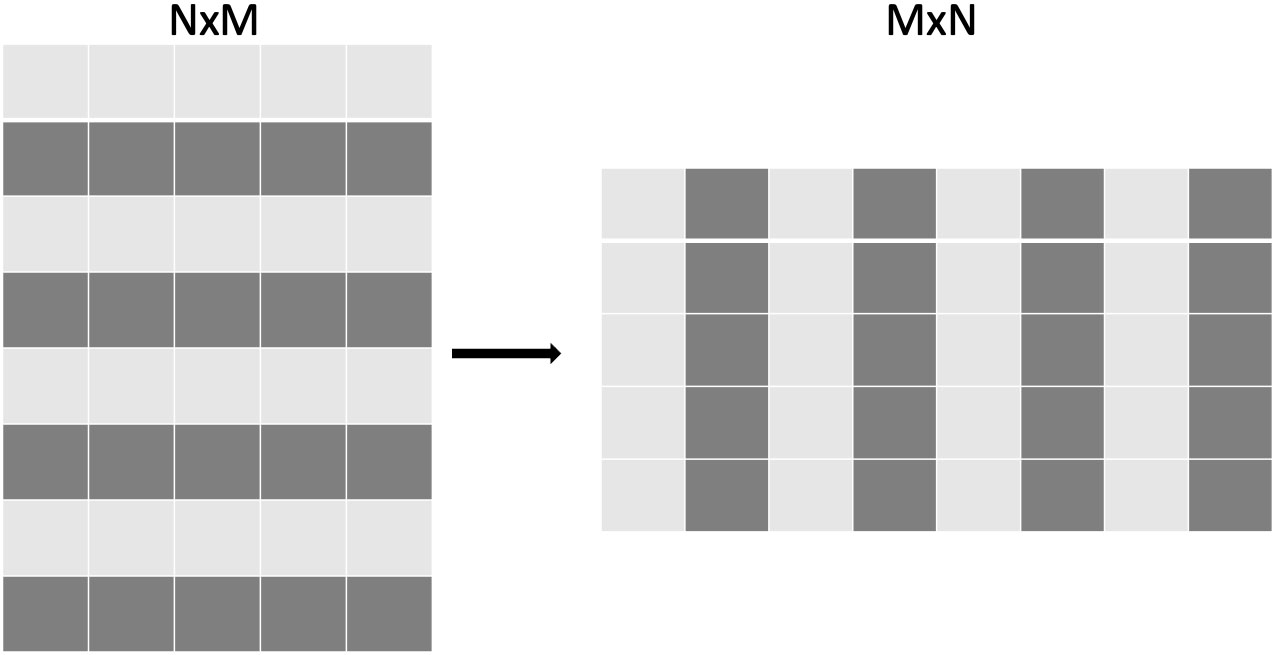
\includegraphics[width=0.8\textwidth]{fig_problem/matrix_transpose_2d.jpg}
\caption{Transpose of a (NxM) matrix to a (MxN) matrix.}\label{fig:matrix_transpose}
\end{figure}


\par
Matrix transpose~\cite{matrix_transpose} is a classic example in GPU programming where shared memory can significantly improve the performance~\cite{matrix_transpose_efficient, matrix_transpose_advanced}.
The use of shared memory reduces global memory accesses and exploits the high bandwidth and low latency of shared memory.
First as a reference we use a simple kernel which copy the data from one array to the other.
The code examples of CUDA, HIP, and SYCL are provided in List~\ref{lst:09_matrix_transpose_cuda}, List~\ref{lst:09_matrix_transpose_hip}, and List~\ref{lst:09_matrix_transpose_sycl}, respectively.


\lstinputlisting[language=c++, caption={The~\lq\lq Matrix Transpose\rq\rq~example of CUDA.}, label={lst:09_matrix_transpose_cuda}, xleftmargin=0.05\textwidth, xrightmargin=0.05\textwidth]{code_examples/09_matrix_transpose_cuda.cpp}


\lstinputlisting[language=c++, caption={The~\lq\lq Matrix Transpose\rq\rq~example of HIP.}, label={lst:09_matrix_transpose_hip}, xleftmargin=0.05\textwidth, xrightmargin=0.05\textwidth]{code_examples/09_matrix_transpose_hip.cpp}


\lstinputlisting[language=c++, caption={The~\lq\lq Matrix Transpose\rq\rq~example of SYCL.}, label={lst:09_matrix_transpose_sycl}, xleftmargin=0.05\textwidth, xrightmargin=0.05\textwidth]{code_examples/09_matrix_transpose_sycl.cpp}


\par
It should be noted that there is no calculations in these code examples.
Each thread reads one element and then writes it to another location.
By measuring the execution time of the kernel, we can compute the effective bandwidth achieve by this kernel.
Herein, we can measure the time using~\textbf{rocprof} or~\textbf{cuda/hip events}.
On a NVIDIA V100 GPU this code achieves 717 GB/s out of the theoretical peak 900 GB/s.


\par
Now we do the first iteration of the code, a~\textbf{naive transpose}.
The reading kernels in these code examples have a nice coalesced access pattern, but the writings in these code samples is very inefficient.


\par
Checking the index $in\_index$ in List~\ref{lst:09_matrix_transpose_naive_kernel_cudahip} for CUDA/HIP and List~\ref{lst:09_matrix_transpose_naive_kernel_sycl} for SYCL, we see that two adjacent threads ($threadIdx.x$, and $threadIdx.x+1$) access location in memory near each other.
However the writes are not.
Threads access data which in a strided way.
Two adjacent threads access data separated by $height$ elements.
This practically results in 32 memory operations, however due to under the hood optimizations the achieved bandwidth is 311 GB/s.


\lstinputlisting[language=c++, caption={The $transpose\_naive\_kernel$ in the~\lq\lq Matrix Transpose\rq\rq~example of CUDA/HIP.}, label={lst:09_matrix_transpose_naive_kernel_cudahip}, xleftmargin=0.05\textwidth, xrightmargin=0.05\textwidth]{code_examples/09_matrix_transpose_naive_kernel_cudahip.cpp}

\lstinputlisting[language=c++, caption={The $transposeKernel$ in the~\lq\lq Matrix Transpose\rq\rq~example of SYCL.}, label={lst:09_matrix_transpose_naive_kernel_sycl}, xleftmargin=0.05\textwidth, xrightmargin=0.05\textwidth]{code_examples/09_matrix_transpose_naive_kernel_sycl.cpp}


\par
We can improve the code efficiency by reading the data in a coalesced way, save it in the shared memory row by row and then write in the global memory column by column~\cite{matrix_transpose_efficient, matrix_transpose_advanced}.
The detailed code examples are shown in List~\ref{lst:09_matrix_transpose_sm_kernel_cudahip} for CUDA/HIP and List~\ref{lst:09_matrix_transpose_sm_kernel_sycl} for SYCL.


\lstinputlisting[language=c++, caption={The $transpose\_SM\_kernel$ in the~\lq\lq Matrix Transpose\rq\rq~example of CUDA/HIP.}, label={lst:09_matrix_transpose_sm_kernel_cudahip}, xleftmargin=0.05\textwidth, xrightmargin=0.05\textwidth]{code_examples/09_matrix_transpose_sm_kernel_cudahip.cpp}

\lstinputlisting[language=c++, caption={The $transposeKernel$ in the~\lq\lq Matrix Transpose\rq\rq~example of SYCL.}, label={lst:09_matrix_transpose_sm_kernel_sycl}, xleftmargin=0.05\textwidth, xrightmargin=0.05\textwidth]{code_examples/09_matrix_transpose_sm_kernel_sycl.cpp}


\par
In these two code examples, we define a $tile\_dim$ constant to determine the size of the shared memory tile.
The matrix transpose kernel uses a 2D grid of thread blocks, where each thread block operates on a $tile\_dim$ x $tile\_dim$ tile of the input matrix.

\par
The kernel first loads data from the global memory into the shared memory tile.
Each thread loads a single element from the input matrix into the shared memory tile.
Then, a~\textbf{\textcolor{red}{\_\_syncthreads()}} barrier ensures that all threads have finished loading data into shared memory before proceeding.


\par
Next, the kernel writes the transposed data from the shared memory tile back to the output matrix in global memory.
Each thread writes a single element from the shared memory tile to the output matrix.
By using shared memory, this optimized implementation reduces global memory accesses and exploits memory coalescence, resulting in improved performance compared to a naive transpose implementation.
This kernel achieved on NVIDIA V100 674 GB/s, which is pretty close to the bandwidth achieved by the simple copy kernel, but there is one more thing to improve.


\par
Shared memory is composed of~\textbf{banks}.
Each bank can service only one request at the time.
Bank conflicts happen when more than 1 thread in a specific warp try to access data in bank.
The bank conflicts are resolved by serializing the accesses resulting in less performance.
In the above examples when data are saved to the shared memory, each thread in the warp will save an element of the data in a different one.
Assuming that shared memory has 16 banks after writing each bank will contain one column.
At the last step when we write from the shared memory to the global memory each warp load data from the same bank.
A simple way to avoid this is by just padding the temporary array.
By padding the array, the data is slightly shifting it resulting in no bank conflicts~\cite{matrix_transpose_efficient, matrix_transpose_advanced}.
The effective bandwidth for this kernel is 697 GB/s.
The detailed code examples without bank conflicts are shown in List~\ref{lst:09_matrix_transpose_sm_nobc_kernel_cudahip} for CUDA/HIP and List~\ref{lst:09_matrix_transpose_sm_nobc_kernel_sycl} for SYCL.


\lstinputlisting[language=c++, caption={The $transpose\_SM\_nobc\_kernel$ in the~\lq\lq Matrix Transpose\rq\rq~example of CUDA/HIP.}, label={lst:09_matrix_transpose_sm_nobc_kernel_cudahip}, xleftmargin=0.05\textwidth, xrightmargin=0.05\textwidth]{code_examples/09_matrix_transpose_sm_nobc_kernel_cudahip.cpp}

\lstinputlisting[language=c++, caption={The $transposeKernel$ in the~\lq\lq Matrix Transpose\rq\rq~example of SYCL.}, label={lst:09_matrix_transpose_sm_nobc_kernel_sycl}, xleftmargin=0.05\textwidth, xrightmargin=0.05\textwidth]{code_examples/09_matrix_transpose_sm_nobc_kernel_sycl.cpp}


\par
A short summary of using the sharing memory as a cache in GPU programming.
\begin{itemize}
    \item Shared memory can significantly improve performance in operations like matrix transpose.
    \item Shared memory reduces global memory accesses and exploits the high bandwidth and low latency of shared memory.
    \item An optimized implementation utilizes shared memory, loads data coalescedly, and performs transpose operations.
    \item The optimized implementation uses a 2D grid of thread blocks and a shared memory tile size determined by a constant.
    \item The kernel loads data from global memory into the shared memory tile and uses a synchronization barrier.
    \item To avoid bank conflicts in shared memory, padding the temporary array is a simple solution.
\end{itemize}


% ---------------------------------------------------------------------- %


\subsection{Reduction}


\par
\textbf{Reduction} refers to an operation in which the elements of an array are aggregated in a single value through operations such as summing, finding the maximum or minimum, or performing logical operations.


\par
In the serial approach, the reduction is performed sequentially by iterating through the collection of values and accumulating the result step by step.
This will be enough for small sizes, but for big problems this results in significant time spent in this part of an application.
On a GPU, this approach is not feasible. Using just one thread to do this operation means the rest of the GPU is wasted.
Doing reduction in parallel is a little tricky.
In order for a thread to do work, it needs to have some partial result to use.
If we launch, for example, a kernel performing a simple vector summation, $sum[0] += a[tid]$, with $N$ threads we notice that this would result in undefined behaviour.
GPUs have mechanisms to access the memory and lock the access for other threads while one thread is doing some operations to a given data via~\textbf{atomics}, however this means that the memory access gets again to be serialized.
There is not much gain.
We note that when doing reductions the order of the iterations is not important (barring the typical non-associative behavior of floating-point operations).
Also we might have to divide the problem into several subsets and do the reduction operation for each subset separately.
On the GPUs, since the GPU threads are grouped in blocks, the size of the subset based on that.
Inside the block, threads can cooperate with each other, they can share data via the shared memory and can be synchronized as well.
All threads read the data to be reduced, but now we have significantly less partial results to deal with.
In general, the size of the block ranges from 256 to 1024 threads.
In case of very large problems, after this procedure if we are left too many partial results this step can be repeated.


\par
At the block level we still have to perform a reduction in an efficient way.
Doing it serially means that we are not using all GPU cores (roughly 97\% of the computing capacity is wasted). 
Doing it naively parallel using~\textbf{atomics}, but on the shared memory is also not a good option.
Going back to the fact the reduction operation is commutative and associative we can set each thread to~\lq\lq reduce\rq\rq~two elements of the local part of the array.
Shared memory can be used to store the partial~\lq\lq reductions\rq\rq~as shown below in the code examples of List~\ref{lst:09_reduction_cudahip} for CUDA/HIP and List~\ref{lst:09_reduction_sycl} for SYCL.


\lstinputlisting[language=c++, caption={The $reduction\_one$ kernel in the~\lq\lq Reduction\rq\rq~example of CUDA/HIP.}, label={lst:09_reduction_cudahip}, xleftmargin=0.05\textwidth, xrightmargin=0.05\textwidth]{code_examples/09_reduction_cudahip.cpp}

\lstinputlisting[language=c++, caption={The $reductionKernel$ in the~\lq\lq Reduction\rq\rq~example of SYCL.}, label={lst:09_reduction_sycl}, xleftmargin=0.05\textwidth, xrightmargin=0.05\textwidth]{code_examples/09_reduction_sycl.cpp}


\par
In the kernel we have each GPU performing thread a reduction of two elements from the local portion of the array.
If we have $tpb$ GPU threads per block, we utilize them to store $2 * tpb$ elements in the local shared memory.
To ensure synchronization until all data is available in the shared memory, we employ the~\textbf{\textcolor{red}{\_\_syncthreads()}} function.


\par
Next, we instruct each thread to~\lq\lq reduce\rq\rq~the element in the array at $threadIdx.x$ with the element at $threadIdx.x + tpb$.
As this operation saves the result back into the shared memory, we once again employ the~\textbf{\textcolor{red}{\_\_syncthreads()}} function.
By doing this, we effectively halve the number of elements to be reduced.


\par
This procedure can be repeated, but now we only utilize $tpb / 2$ threads.
Each thread is responsible for~\lq\lq reducing\rq\rq~the element in the array at $threadIdx.x$ with the element at $threadIdx.x + tpb / 2$.
After this step, we are left with $tpb / 4$ numbers to be reduced.
We continue applying this procedure until only one number remains, as shown in Fig.~\ref{fig:reduction}.


\begin{figure}[htbp]
\centering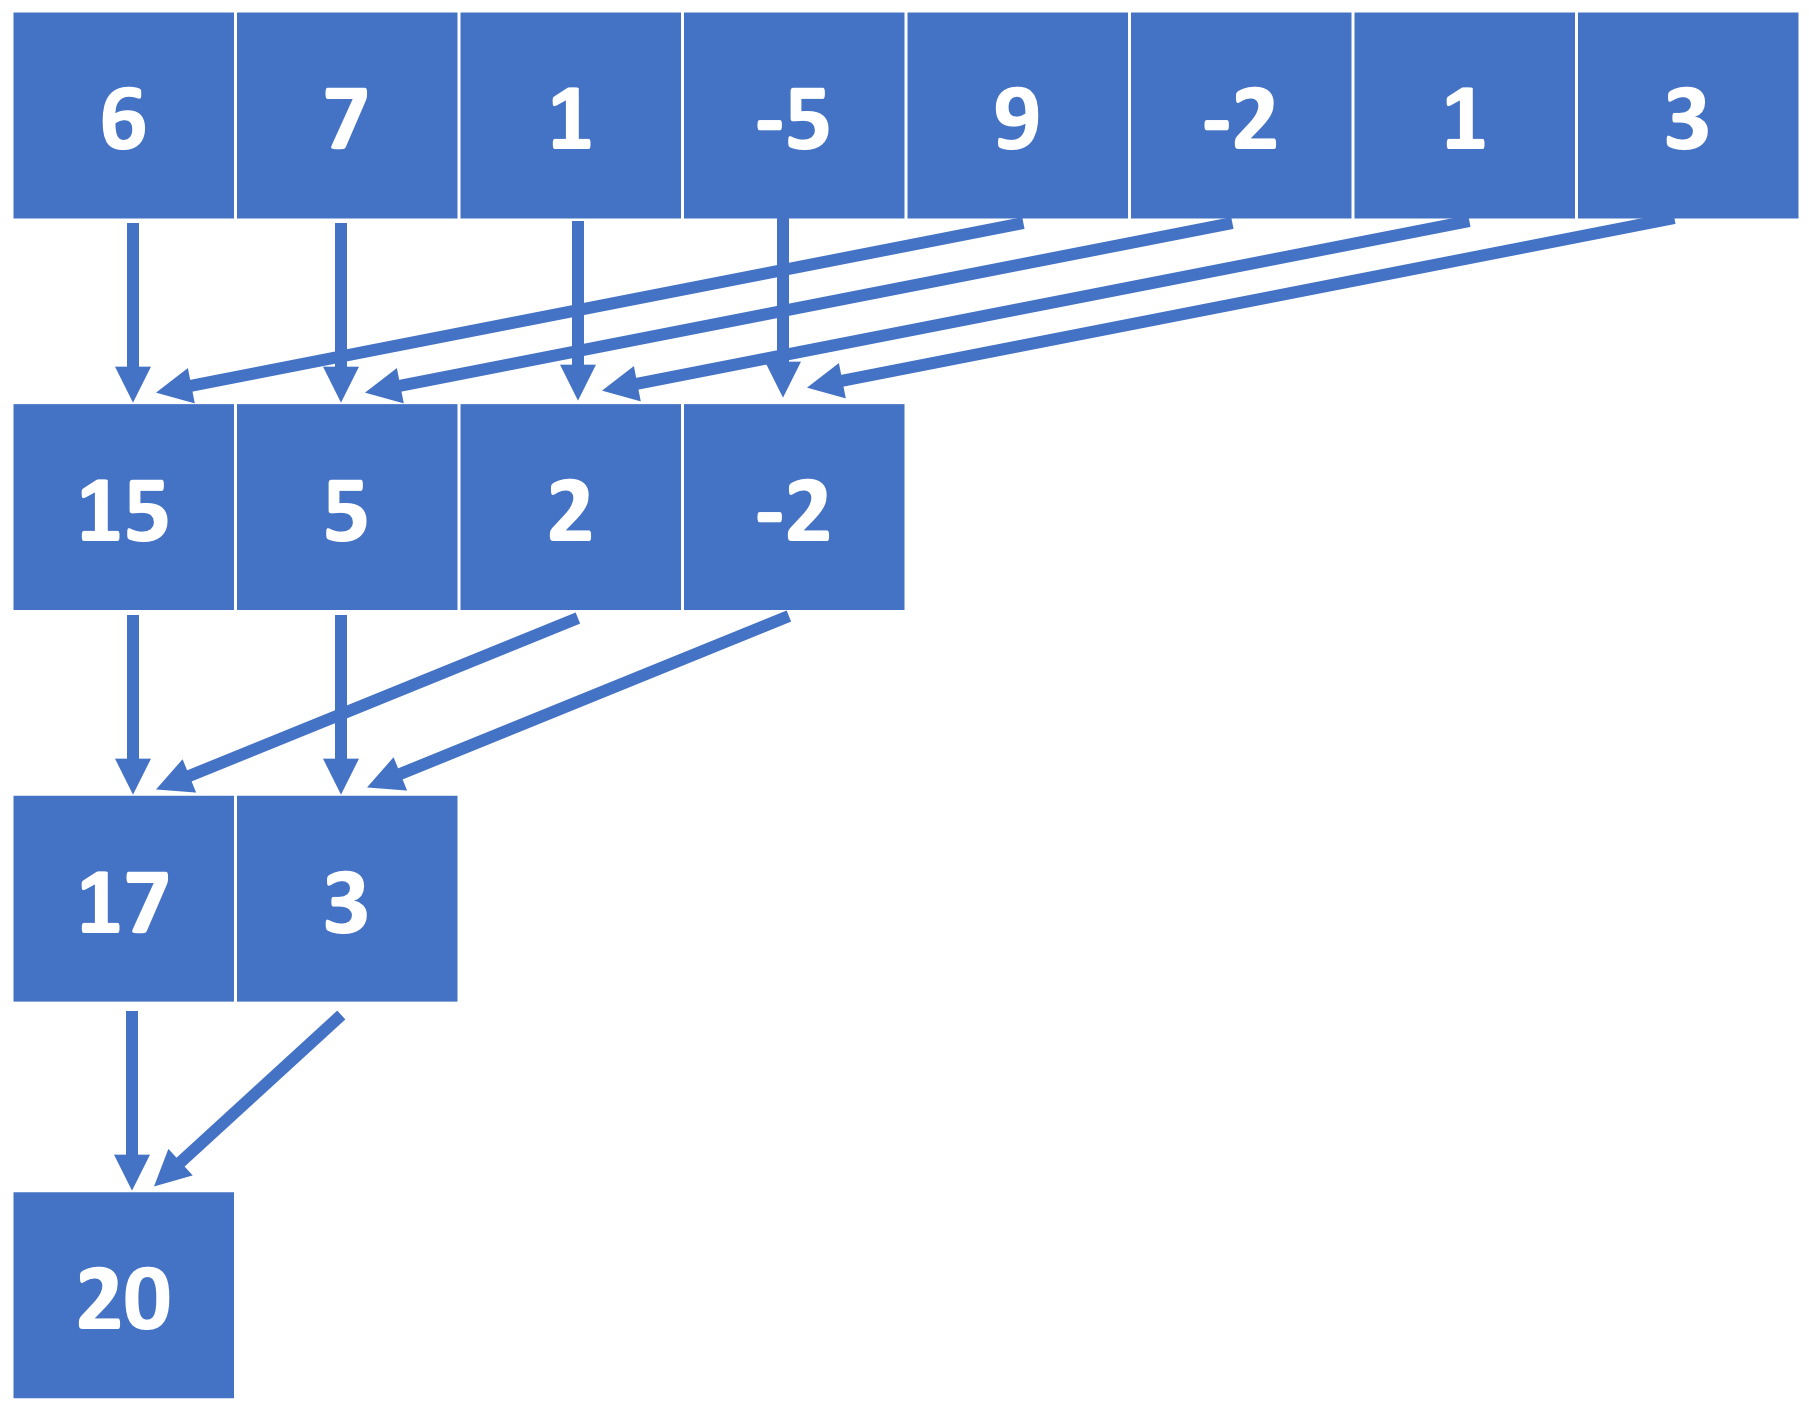
\includegraphics[width=0.6\textwidth]{fig_problem/reduction.png}
\caption{Schematic representation on the reduction algorithm with 8 GPU threads.}\label{fig:reduction}
\end{figure}


\par
At this point, we can either~\lq\lq reduce\rq\rq~the final number with a global partial result using~\textbf{atomic} read and write operations, or we can save it into an array for further processing.
For a detail analysis of how to optimize reduction operations in CUDA/HIP check the presentation~\href{https://developer.download.nvidia.com/assets/cuda/files/reduction.pdf}{Optimizing Parallel Reduction in CUDA}.


\par
Here is a short summary for reduction.
\begin{itemize}
    \item Reductions refer to aggregating elements of an array into a single value through operations like summing, finding maximum or minimum, or performing logical operations.
    \item Performing reductions sequentially in a serial approach is inefficient for large problems, while parallel reduction on GPUs offers better performance.
    \item Parallel reduction on GPUs involves dividing the problem into subsets, performing reductions within blocks of threads using shared memory, and repeatedly reducing the number of elements (two per GPU thread) until only one remains.
\end{itemize}


% ---------------------------------------------------------------------- %


\subsection{CUDA/HIP Streams}


\par
Modern GPUs can overlap independent operations.
They can do transfers between CPU and GPU and execute kernels in the same time, or they can execute kernels concurrently.
CUDA/HIP streams are independent execution units, a sequence of operations that execute in issue-order on the GPU.
The operations issue in different streams can be executed concurrently.


\par
Consider the case of~\lq\lq Vector Addition\rq\rq~discussed in previous subsection~\ref{sec:vector_addition}, which involves copying data from CPU to GPU, computations and then copying back the result to GPU, as shown in Fig.~\ref{fig:streams_timeline}.
In this way nothing can be overlapped.


\begin{figure}[htbp]
\centering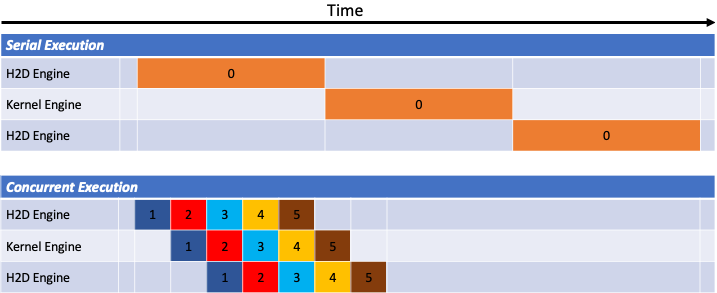
\includegraphics[width=0.8\textwidth]{fig_problem/streams_timeline.png}
\caption{The stream timelines for serial and concurrent executions in GPU programming.}\label{fig:streams_timeline}
\end{figure}


\par
We can improve the performance by dividing the problem into smaller independent parts.
Herein we consider 5 streams assuming the case where copy in one direction and computation take the same amount of time, as shown in Fig.~\ref{fig:streams_timeline}.
After the first and second stream copy data to the GPU, the GPU is practically occupied all time.
We can see that significant performance improvements can be obtained by eliminating the time in which the GPU is idle, waiting for data to arrive from the CPU.
This very useful for problems where there is often communication to the CPU because the GPU memory can not fit all the problem or the application runs in a multi-GPU set up and communication is needed often.


\par
We can apply this method to the~\lq\lq Vector Addition\rq\rq~program to expect the improvement of code examples of List~\ref{lst:09_vector_addition_stream_cuda} for CUDA and List~\ref{lst:09_vector_addition_stream_hip} for HIP.


\lstinputlisting[language=c++, caption={The application of stream method in the~\lq\lq Vector Addition\rq\rq~example of CUDA.}, label={lst:09_vector_addition_stream_cuda}, xleftmargin=0.05\textwidth, xrightmargin=0.05\textwidth]{code_examples/09_vector_addition_stream_cuda.cpp}

\lstinputlisting[language=c++, caption={The application of stream method in the~\lq\lq Vector Addition\rq\rq~example of HIP.}, label={lst:09_vector_addition_stream_hip}, xleftmargin=0.05\textwidth, xrightmargin=0.05\textwidth]{code_examples/09_vector_addition_stream_hip.cpp}


\par
It is clearly shown in these code examples that instead of having one copy to GPU, one execution of the kernel and one copy back, we now have several of these calls independent of each other.
Note that even when streams are not explicitly used, it is possible to launch all the GPU operations asynchronous and overlap CPU operations (such I/O) and GPU operations.
In order to learn more about how to improve performance using CUDA/HIP streams, one should check the NVIDIA blog\href{https://developer.nvidia.com/blog/how-overlap-data-transfers-cuda-cc/}{How to Overlap Data Transfers in CUDA C/C++}.


\par
Here is a short summary for CUDA/HIP streams.
\begin{itemize}
    \item CUDA/HIP streams are independent execution contexts on the GPU that allow for concurrent execution of operations issued in different streams.
    \item Using streams can improve GPU performance by overlapping operations such as data transfers between CPU and GPU and kernel executions.
    \item By dividing a problem into smaller independent parts and utilizing multiple streams, the GPU can avoid idle time, resulting in significant performance improvements, especially for problems with frequent CPU communication or multi-GPU setups.
\end{itemize}


% ---------------------------------------------------------------------- %


\subsection{Pros and cons of native programming models}


\par
There are advantages and limitations to native GPU programming models of CUDA and HIP:
\begin{itemize}
    \item~\textbf{CUDA Pros}:
    \begin{itemize}
        \item Performance Boost: CUDA is designed for NVIDIA GPUs and delivers excellent performance.
        \item Wide Adoption: CUDA is popular, with many resources and tools available.
        \item Mature Ecosystem: NVIDIA provides comprehensive libraries and tools for CUDA programming.
    \end{itemize}
    \item~\textbf{HIP Pros}:
    \begin{itemize}
        \item Portability: HIP is portable across different GPU architectures.
        \item Open Standards: HIP is based on open standards, making it more accessible.
        \item Growing Community: The HIP community is growing, providing more resources and support.
    \end{itemize}
    \item~\textbf{Cons}:
    \begin{itemize}
        \item Exclusive for GPUs
        \item Vendor Lock-in: CUDA is exclusive to NVIDIA GPUs, limiting compatibility.
        \item Learning Curve: Both CUDA and HIP require learning GPU programming concepts.
        \item Limited Hardware Support: HIP may face limitations on older or less common GPUs.
    \end{itemize}
\end{itemize}


\section{Portable Kernel-Based Programming Models}\label{sec:portable-kernel-based-programming-models}


\par
The goal of the cross-platform portability ecosystems is to allow the same code to run on multiple architectures, therefore reducing code duplication.
They are usually based on C++, and use function objects/lambda functions to define the loop body ($i.e.$, the kernel), which can run on multiple architectures like CPU, GPU, and FPGA from different vendors.
An exception to this is OpenCL, which originally offered only a C API (although currently the C++ API is available), and uses a separate-source model for the kernel code. 
However, unlike in many conventional CUDA or HIP implementations, the portability ecosystems require kernels to be written only once if one prefers to run it on CPU and GPU for example.
Some notable cross-platform portability ecosystems are Alpaka~\cite{alpaka}, Kokkos~\cite{kokkos}, OpenCL~\cite{OpenCL}, RAJA~\cite{raja}, and SYCL~\cite{sycl}.
Alpaka, Kokkos and RAJA are individual projects whereas OpenCL and SYCL are standards followed by several projects implementing (and extending) them.
For example, some notable SYCL implementations include Intel oneAPI DPC++~\cite{oneapi-dpc}, hipSYCL (also known as Open SYCL)~\cite{hipsycl}, triSYCL~\cite{trisycl}, and ComputeCPP~\cite{computecpp}.


% ---------------------------------------------------------------------- %


\subsection{Kokkos}


\par
Kokkos is an open-source performance portability ecosystem for parallelization on large heterogeneous hardware architectures of which development has mostly taken place on Sandia National Laboratories~\cite{kokkos, kokkos_sandia}.
The project started in 2011 as a parallel C++ programming model, but have since expanded into a more broad ecosystem including Kokkos Core (the programming model), Kokkos Kernels (math library), and Kokkos Tools (debugging, profiling and tuning tools).
By preparing proposals for the C++ standard committee, the project also aims to influence the ISO/C++ language standard such that, eventually, Kokkos capabilities will become native to the language standard.
Here is a more detailed introduction of~\href{https://www.sandia.gov/news/publications/hpc-annual-reports/article/kokkos/}{The Kokkos EcoSystem}.


\par
The Kokkos library provides an abstraction layer for a variety of different parallel programming models, currently CUDA, HIP, SYCL, HPX, OpenMP, and C++ threads.
Therefore, it allows better portability across different hardware manufactured by different vendors, but introduces an additional dependency to the software stack.
For example, when using CUDA, only CUDA installation is required, but when using Kokkos with NVIDIA GPUs, Kokkos and CUDA installation are both required.
Kokkos is not a very popular choice for parallel programming, and therefore, learning and using Kokkos can be more difficult compared to more established programming models such as CUDA, for which a much larger amount of search results and~\href{https://stackoverflow.com/}{Stack Overflow} discussions can be found.


\subsubsection{Kokkos compilation}


\par
Furthermore, one challenge with some cross-platform portability libraries is that even on the same system, different projects may require different combinations of compilation settings for the portability library.
For example, in Kokkos, one project may wish the default execution space to be a CUDA device, whereas another requires a CPU.
Even if the projects prefer the same execution space, one project may desire the unified memory to be the default memory space and the other may wish to use pinned GPU memory. 
It may be burdensome to maintain a large number of library instances on a single system.


\par
However, Kokkos offers a simple way to compile Kokkos library simultaneously with the user project.
This is achieved by specifying Kokkos compilation settings~\cite{kokkos_compiling} and including the Kokkos Makefile in the user Makefile.
\textbf{CMake} is also supported.
This way, the user application and Kokkos library are compiled together.
The code in List~\ref{lst:10_kokkos_hello_makefile} is an example Makefile for a single-file Kokkos project (\textbf{\textcolor{brown}{hello.cpp}} as shown in List~\ref{lst:10_kokkos_hello}) that uses CUDA (Volta architecture) as the backend (default execution space) and Unified Memory as the default memory space.
To build this Kokkos project (\textbf{\textcolor{brown}{hello.cpp}} in List~\ref{lst:10_kokkos_hello}) with the above Makefile, no steps other than cloning the Kokkos project into the current directory is required.


\lstinputlisting[language=bash, caption={An example Makefile for a single-file Kokkos project (\textbf{\textcolor{brown}{hello.cpp}}) shown in List~\ref{lst:10_kokkos_hello}.}, label={lst:10_kokkos_hello_makefile}, xleftmargin=0.05\textwidth, xrightmargin=0.05\textwidth]{code_examples/10_kokkos_hello_makefile.cpp}


\lstinputlisting[language=c++, caption={A single-file Kokkos project (\textbf{\textcolor{brown}{hello.cpp}}).}, label={lst:10_kokkos_hello}, xleftmargin=0.05\textwidth, xrightmargin=0.05\textwidth]{code_examples/10_kokkos_hello.cpp}


\subsubsection{Kokkos programming}


\par
When starting to write a project using Kokkos, the first step is understand Kokkos initialization and finalization.
Kokkos must be initialized by calling~\textbf{\textcolor{red}{Kokkos::initialize(int argc, char * argv[])}} and finalized by calling~\textbf{\textcolor{red}{Kokkos::finalize()}}.
More details about the~\href{https://kokkos.github.io/kokkos-core-wiki/ProgrammingGuide/Initialization.html}{Kokkos initialization} are given at the~\href{https://kokkos.github.io/kokkos-core-wiki/index.html}{Kokkos documentation}.


\par
Kokkos uses an execution space model to abstract the details of parallel hardware.
The execution space instances map to the available backend options such as CUDA, OpenMP, HIP, or SYCL.
If the execution space is not explicitly chosen by the programmer in the source code, the default execution space~\textbf{\textcolor{red}{Kokkos::DefaultExecutionSpace}} is used. 
This is chosen when the Kokkos library is compiled.
One should refers to the~\href{https://kokkos.github.io/kokkos-core-wiki/ProgrammingGuide/Machine-Model.html#}{Machine Model} section in the ~\href{https://kokkos.github.io/kokkos-core-wiki/index.html}{Kokkos documentation} for detailed information of the Kokkos execution space model.


\par
Similarly, Kokkos uses a memory space model for different types of memory, such as host memory or device memory.
If not defined explicitly, Kokkos uses the default memory space specified during Kokkos compilation.
The detailed description of the~\href{https://kokkos.github.io/kokkos-core-wiki/ProgrammingGuide/Machine-Model.html#kokkos-memory-spaces}{Kokkos Memory Spaces} is available at the~\href{https://kokkos.github.io/kokkos-core-wiki/index.html}{Kokkos documentation}.


\par
The code in List~\ref{lst:10_kokkos_hello} is an example of a single-file Kokkos program (\textbf{\textcolor{brown}{hello.cpp}}) that initializes Kokkos and prints the execution space and memory space instances.
With Kokkos, the data can be accessed either through raw pointers or through~\textbf{Kokkos Views}.
With raw pointers, the memory allocation into the default memory space can be done using~\textbf{\textcolor{red}{Kokkos::kokkos\_malloc(n * sizeof(int))}}.
Kokkos Views are a data type that provides a way to access data more efficiently in memory corresponding to a certain Kokkos memory space, such as host memory or device memory. 
A one-dimensional view of type $int *$ can be created by~\textbf{\textcolor{red}{Kokkos::View$<$int *$>$ a("a", n)}}, where $"a"$ is a label, and $n$ is the size of the allocation in the number of integers.
Kokkos determines the optimal layout for the data at compile time for best overall performance as a function of the computer architecture.
Furthermore, Kokkos handles the deallocation of such memory automatically.
More details about the~\href{https://kokkos.github.io/kokkos-core-wiki/ProgrammingGuide/View.html}{Kokkos Views} are available at the~\href{https://kokkos.github.io/kokkos-core-wiki/index.html}{Kokkos documentation}.


\par
Finally, Kokkos provides three different parallel operations:~\textbf{\textcolor{red}{parallel\_for}},~\textbf{\textcolor{red}{parallel\_reduce}}, and~\textbf{\textcolor{red}{parallel\_scan}}.
The~\textbf{\textcolor{red}{parallel\_for}} operation is used to execute a loop in parallel.
The~\textbf{\textcolor{red}{parallel\_reduce}} operation is used to execute a loop in parallel and reduce the results to a single value.
The~\textbf{\textcolor{red}{parallel\_scan}} operation implements a prefix scan.
The usage of~\textbf{\textcolor{red}{parallel\_for}} and~\textbf{\textcolor{red}{parallel\_reduce}} are demonstrated in the examples later in this section.
More detail about the~\href{https://kokkos.github.io/kokkos-core-wiki/ProgrammingGuide/ParallelDispatch.html}{Kokkos parallel operations} are available at the~\href{https://kokkos.github.io/kokkos-core-wiki/index.html}{Kokkos documentation}.


\subsubsection{Kokkos running examples}


\par
The following simple steps (List~\ref{lst:10_kokkos_git}) should work on AMD VEGA90A device straight out of the box (needs ROCM installation).
On NVIDIA Volta V100 device (needs CUDA installation), use the variables commented out on the Makefile.


\lstinputlisting[language=fortran, caption={Simple commands to run the~\textbf{\textcolor{brown}{hello.cpp}} file using GPU.}, label={lst:10_kokkos_git}, xleftmargin=0.05\textwidth, xrightmargin=0.05\textwidth]{code_examples/10_kokkos_git.pbs}


% ---------------------------------------------------------------------- %


\subsection{OpenCL}


\par
OpenCL~\cite{OpenCL} is a cross-platform, open-standard API for writing parallel programs that execute across heterogeneous platforms consisting of CPUs, GPUs, FPGAs and other devices.
The first version of OpenCL (1.0) was released in December 2008, and the latest version of OpenCL (3.0) was released in September 2020.
OpenCL is supported by a number of vendors, including AMD, ARM, Intel, NVIDIA, and Qualcomm.
It is a royalty-free standard, and the OpenCL specification is maintained by the Khronos Group~\cite{khronos_group}.
OpenCL provides a low-level programming interface initially based on C, but more recently also a C++ interface has become available.


\subsubsection{OpenCL compilation}


\par
OpenCL supports two modes for compiling the programs: online and offline.
The online compilation occurs at runtime, when the host program calls a function to compile the source code.
The online mode allows dynamic generation and loading of kernels, but may incur some overhead due to compilation time and possible errors.
The offline compilation occurs before runtime, when the source code of a kernel is compiled into a binary format that can be loaded by the host program.
This mode allows faster execution and better optimization of kernels, but may limit the portability of the program, because the binary can only run on the architectures it was compiled for.


\par
OpenCL comes bundled with several parallel programming ecosystems, such as NVIDIA CUDA and Intel oneAPI.
For example, after successfully installing such packages and setting up the environment, one may simply compile an OpenCL program by the commands such as~\textbf{\textcolor{brown}{icx cl\_devices.c -lOpenCL}} (Intel oneAPI) or~\textbf{\textcolor{brown}{nvcc cl\_devices.c -lOpenCL}} (NVIDIA CUDA), where~\textbf{\textcolor{brown}{cl\_devices.c}} is the compiled file.
Unlike most other programming models, OpenCL stores kernels as text and compiles them for the device in runtime (JIT-compilation), and thus does not require any special compiler support: one can compile the code using simply~\textbf{\textcolor{brown}{gcc cl\_devices.c -lOpenCL}} (or~\textbf{\textcolor{brown}{g++}} when using C++ API), as long as the required libraries and headers are installed in a standard location.


\par
The AMD compiler installed on LUMI supports both OpenCL C and C++ APIs, the latter with some limitations.
To compile a program, you can use the AMD compilers (List~\ref{lst:10_opencl_compiler_lumi})) on a GPU partition


\lstinputlisting[language=bash, caption={The adopted AMD compilers on the LUMI GPU partition to compile a C/C++ programe using OpenCL.}, label={lst:10_opencl_compiler_lumi}, xleftmargin=0.05\textwidth, xrightmargin=0.05\textwidth]{code_examples/10_opencl_compiler_lumi.pbs}


\subsubsection{OpenCL programming}


\par
OpenCL programs consist of two parts: a host program that runs on the host device (usually a CPU) and one or more kernels that run on compute devices (such as GPUs).
The host program is responsible for the tasks such as managing the devices for the selected platform, allocating memory objects, building and enqueueing kernels, and managing memory objects.


\par
The first steps when writing an OpenCL program are to initialize the OpenCL environment by selecting the platform and devices, creating a context or contexts associated with the selected device(s), and creating a command queue for each device.
A simple example of OpenCL initialization for selecting the default device, creating a context and a queue associated with the device is shown in List~\ref{lst:10_opencl_initialization_c_api} for C and List~\ref{lst:10_opencl_initialization_cpp_api} for C++ APIs.


\lstinputlisting[language=c, caption={A code example for C API to select the default GPU device, creating a context and a queue associated with the GPU device.}, label={lst:10_opencl_initialization_c_api}, xleftmargin=0.05\textwidth, xrightmargin=0.05\textwidth]{code_examples/10_opencl_initialization_c_api.c}


\lstinputlisting[language=c++, caption={A code example for C++ API to select the default GPU device, creating a context and a queue associated with the GPU device.}, label={lst:10_opencl_initialization_cpp_api}, xleftmargin=0.05\textwidth, xrightmargin=0.05\textwidth]{code_examples/10_opencl_initialization_cpp_api.cpp}


\par
OpenCL provides two main programming models to manage the memory hierarchy of host and accelerator devices: buffers and shared virtual memory (SVM).
Buffers are the traditional memory model of OpenCL, where the host and the devices have separate address spaces and the programmer has to explicitly specify the memory allocations and how and where the memory is accessed. This can be done with class \textbf{\textcolor{red}{cl::Buffer}} and functions such as \textbf{\textcolor{red}{cl::CommandQueue::enqueueReadBuffer()}}.
Buffers are supported since early versions of OpenCL, and work well across different architectures.
Buffers can also take advantage of device-specific memory features, such as constant or local memory.


\par
SVM is a newer memory model of OpenCL, introduced in version 2.0, where the host and the devices share a single virtual address space.
Thus, the programmer can use the same pointers to access the data from host and devices simplifying the programming effort.
In OpenCL, SVM comes in different levels such as coarse-grained buffer SVM, fine-grained buffer SVM, and fine-grained system SVM.
All levels allow using the same pointers across a host and devices, but they differ in their granularity and synchronization requirements for the memory regions.
Furthermore, the support for SVM is not universal across all OpenCL platforms and devices.
For example, GPUs such as NVIDIA V100 and A100 only support the coarse-grained SVM buffer.
This level requires explicit synchronization for memory accesses from a host and devices (using functions such as~\textbf{\textcolor{red}{cl::CommandQueue::enqueueMapSVM()}} and~\textbf{\textcolor{red}{cl::CommandQueue::enqueueUnmapSVM()}}), making the usage of SVM less convenient.
It is further noted that this is unlike the regular Unified Memory offered by CUDA, which is closer to the fine-grained system SVM level in OpenCL.


\par
OpenCL uses a separate-source kernel model where the kernel code is often kept in separate files that may be compiled during runtime.
The model allows the kernel source code to be passed as a string to the OpenCL driver after which the program object can be executed on a specific device.
Although referred to as the separate-source kernel model, the kernels can still be defined as a string in the host program compilation units as well, which may be a more convenient approach in some cases.


\par
The online compilation with the separate-source kernel model has several advantages over the binary model, which requires offline compilation of kernels into device-specific binaries that can be loaded by the application at runtime.
The online compilation preserves the portability and flexibility of OpenCL, as the same kernel source code can run on any supported device.
Furthermore, dynamic optimization of kernels based on runtime information, such as input size, work-group size, or device capabilities, is possible.
An example of an OpenCL kernel, defined by a string in the host compilation unit, and assigning the global thread index into a global device memory is shown in List~\ref{lst:10_opencl_kernel_example}.


\lstinputlisting[language=c, caption={An code example of an OpenCL kernel defined by a string in host compilation unit and assigning global thread index into a global device memory.}, label={lst:10_opencl_kernel_example}, xleftmargin=0.05\textwidth, xrightmargin=0.05\textwidth]{code_examples/10_opencl_kernel_example.cpp}


\par
The above kernel named~\textbf{\textcolor{red}{kernel\_dot}} and stored in the string~\textbf{\textcolor{red}{kernel\_source}} can be set to build in the host code for C (List~\ref{lst:10_opencl_kernel_build_example_c_api}) and C++ (List~\ref{lst:10_opencl_kernel_build_example_cpp_api}) APIs.


\lstinputlisting[language=c, caption={A code example containing an OpenCL kernel (\textbf{\textcolor{red}{kernel\_dot}}) stored in the string~\textbf{\textcolor{red}{kernel\_source}} to build in the host code for C API.}, label={lst:10_opencl_kernel_build_example_c_api}, xleftmargin=0.05\textwidth, xrightmargin=0.05\textwidth]{code_examples/10_opencl_kernel_build_example_c_api.c}


\lstinputlisting[language=c++, caption={A code example containing an OpenCL kernel (\textbf{\textcolor{red}{kernel\_dot}}) stored in the string~\textbf{\textcolor{red}{kernel\_source}} to build in the host code for C++ API.}, label={lst:10_opencl_kernel_build_example_cpp_api}, xleftmargin=0.05\textwidth, xrightmargin=0.05\textwidth]{code_examples/10_opencl_kernel_build_example_cpp_api.cpp}


% ---------------------------------------------------------------------- %


\subsection{SYCL}


\par
SYCL~\cite{sycl} is a royalty-free, open-standard C++ programming model for multi-device programming.
It provides a high-level, single-source programming model for heterogeneous systems, including GPUs.
There are several implementations of the standard.
For GPU programming, Intel oneAPI DPC++~\cite{oneapi-dpc} and hipSYCL~\cite{hipsycl} are the most popular for desktop and HPC GPUs; ComputeCPP~\cite{computecpp} is a good choice for embedded devices.
The same standard-compliant SYCL code should work with any implementation, but they are not binary-compatible.


\par
The most recent version of the SYCL standard is SYCL 2020, and it is the version we will use in this workshop.


\subsubsection{SYCL compilation}


\paragraph{Intel oneAPI DPC++.}
For targeting Intel GPUs, it is enough to install the Intel oneAPI Base Toolkit~\cite{intel_oneapi_base_toolkit}. 
Then, the compilation is as simple as shown below.
\lstinputlisting[language=c++, firstline=5, lastline=5, xleftmargin=0.05\textwidth, xrightmargin=0.05\textwidth]{code_examples/10_sycl_compilation.c}
It is also possible to use oneAPI for NVIDIA and AMD GPUs.
In addition to the Intel oneAPI Base Toolkit, the vendor-provided runtime (CUDA or HIP) and the corresponding Codeplay oneAPI plugin~\cite{codeplay-oneapi} must be installed.
Then, the code can be compiled using Intel LLVM compiler bundled with oneAPI, as shwon below for targeting CUDA 8.6 NVIDIA GPU and for targeting GFX90a AMD GPU.
\lstinputlisting[language=c++, firstline=7, lastline=11, xleftmargin=0.05\textwidth, xrightmargin=0.05\textwidth]{code_examples/10_sycl_compilation.c}


\paragraph{hipSYCL.}
Using hipSYCL for NVIDIA or AMD GPUs also requires having CUDA or HIP installed first.
Then~\textbf{syclcc} can be used for compiling the code, specifying the target devices.
For example, one can use the command below to compile the program supporting an AMD and an NVIDIA device.
\lstinputlisting[language=c++, firstline=20, lastline=20, xleftmargin=0.05\textwidth, xrightmargin=0.05\textwidth]{code_examples/10_sycl_compilation.c}


\paragraph{Using SYCL on LUMI.}
LUMI does not have a system-wide installation of any SYCL framework.
For this course, an installation of hipSYCL 0.9.4 was prepared, which can be loaded via:
\lstinputlisting[language=bash, firstline=28, lastline=31, xleftmargin=0.05\textwidth, xrightmargin=0.05\textwidth]{code_examples/10_sycl_compilation.c}
The default compilation target is preset to MI250 GPUs, so to compile a single C++ file it is enough to use the command below.
\lstinputlisting[language=bash, firstline=35, lastline=35, xleftmargin=0.05\textwidth, xrightmargin=0.05\textwidth]{code_examples/10_sycl_compilation.c}
When running applications built with hipSYCL, one can often see the warning~\lq\lq [hipSYCL Warning] dag\_direct\_scheduler: Detected a requirement that is neither of discard access mode\rq\rq, reflecting the lack of an optimization hint when using buffer-accessor model.
The warning is harmless and can be ignored.


\subsubsection{SYCL programming}


\par
SYCL is, in many aspects, similar to OpenCL, but uses, like Kokkos, a single-source model with kernel lambdas.
To submit a task to device, first a~\textbf{\textcolor{red}{sycl::queue}} must be created, which is used as a way to manage the task scheduling and execution.
In the simplest case, that’s all the initialization one needs, as shown in the code example in List~\ref{lst:10_sycl_programming_main}.


\lstinputlisting[language=c++, caption={A simple code example of SYCL.}, label={lst:10_sycl_programming_main}, xleftmargin=0.05\textwidth, xrightmargin=0.05\textwidth]{code_examples/10_sycl_programming_main.cpp}


\par
If one wants more control, the device can be explicitly specified, or additional properties can be passed to a queue, as shown in the code example in List~\ref{lst:10_sycl_programming_queue}.


\lstinputlisting[language=c++, caption={A simple code example of SYCL with explicitly specified device information.}, label={lst:10_sycl_programming_queue}, xleftmargin=0.05\textwidth, xrightmargin=0.05\textwidth]{code_examples/10_sycl_programming_queue.cpp}


\par
For SYCL, the memory management can be done in two different ways:\textbf{buffer-accessor model} and~\textbf{unified shared memory} (USM).
The choice of the memory management models also influences how the GPU tasks are synchronized.


\par
In the buffer-accessor model, a~\textbf{\textcolor{red}{sycl::buffer}} object is used to represent arrays of data. A buffer is not mapped to any single one memory space, and can be migrated between the GPU and the CPU memory transparently.
The data in~\textbf{\textcolor{red}{sycl::buffer}} cannot be read or written directly, an accessor must be created.
The~\textbf{\textcolor{red}{sycl::accessor}} object specifies the location of data access (host or a certain GPU kernel) and the access mode (read-only, write-only, read-write).
Such an approach allows optimizing task scheduling by building a directed acyclic graph (DAG) of data dependencies: if kernel $A$ creates a write-only accessor to a buffer, and then kernel $B$ is submitted with a read-only accessor to the same buffer, and then a host-side read-only accessor is requested, then it can be deduced that $A$ must complete before $B$ is launched and also that the results must be copied to the host before the host task can proceed, but the host task can run in parallel with kernel $B$.
Since the dependencies between tasks can be built automatically, by default SYCL uses~\textbf{out-of-order queues}: when two tasks are submitted to the same~\textbf{\textcolor{red}{sycl::queue}}, it is not guaranteed that the second one will launch only after the first one completes.
When launching a kernel, accessors must be created, and the code example is shown in List~\ref{lst:10_sycl_programming_accessor}.


\lstinputlisting[language=c++, caption={A simple code example of SYCL with accessors before launching a kernel.}, label={lst:10_sycl_programming_accessor}, xleftmargin=0.05\textwidth, xrightmargin=0.05\textwidth]{code_examples/10_sycl_programming_accessor.cpp}


\par
The buffer-accessor model simplifies many aspects of heterogeneous programming and prevents many synchronization-related bugs, but it only allows very coarse control of data movement and kernel execution.


\par
The USM model is similar to how NVIDIA CUDA or AMD HIP manage memory.
The programmer has to explicitly allocate the memory on the host (\textbf{\textcolor{red}{sycl::malloc\_host}}), on the device (\textbf{\textcolor{red}{sycl::malloc\_device}}), or in the shared memory space (\textbf{\textcolor{red}{sycl::malloc\_shared}} in List~\ref{lst:10_sycl_programming_malloc}).
Despite its name, unified shared memory, and the similarity to OpenCL’s SVM, not all USM allocations are shared.
For example, a memory allocated by\textbf{\textcolor{red}{sycl::malloc\_device}} cannot be accessed from the host.
The allocation functions return memory pointers that can be used directly, without accessors.
This means that the programmer have to ensure the correct synchronization between host and device tasks to avoid data races.
With USM, it is often convenient to use~\textbf{in-order queues} with USM, instead of the default~\textbf{out-of-order queues} for the buffer-accessor model.
More information on USM can be found in the~\href{https://registry.khronos.org/SYCL/specs/sycl-2020/html/sycl-2020.html#sec:usm}{Section 4.8 of SYCL 2020 specification}.


\lstinputlisting[language=c++, caption={A simple code example of SYCL to create a shared (migratable) allocation of n integers in the the shared memory space using~\textbf{\textcolor{red}{sycl::malloc\_shared}}.}, label={lst:10_sycl_programming_malloc}, xleftmargin=0.05\textwidth, xrightmargin=0.05\textwidth]{code_examples/10_sycl_programming_malloc.cpp}


% ---------------------------------------------------------------------- %


\subsection{Examples}


\par
In this subsection, we provide four sets of code examples of Kokkos, OpenCL, and SYCL for the~\textbf{Parallel for with Unified Memory}, the~\textbf{Parallel for with GPU buffers}, the~\textbf{Asynchronous parallel for kernels}, and the~\textbf{Reduction} programs.


\subsubsection{Parallel for with Unified Memory}


\lstinputlisting[language=c++, caption={The code example of Kokkos for the~\textbf{Parallel for with Unified Memory} program.}, label={lst:10_example_parallel_with_unified_memory_kokkos}, xleftmargin=0.05\textwidth, xrightmargin=0.05\textwidth]{code_examples/10_example_parallel_with_unified_memory_kokkos.cpp}


\lstinputlisting[language=c++, caption={The code example of OpenCL for the~\textbf{Parallel for with Unified Memory} program.}, label={lst:10_example_parallel_with_unified_memory_opencl}, xleftmargin=0.05\textwidth, xrightmargin=0.05\textwidth]{code_examples/10_example_parallel_with_unified_memory_opencl.cpp}


\lstinputlisting[language=c++, caption={The code example of SYCL for the~\textbf{Parallel for with Unified Memory} program.}, label={lst:10_example_parallel_with_unified_memory_sycl}, xleftmargin=0.05\textwidth, xrightmargin=0.05\textwidth]{code_examples/10_example_parallel_with_unified_memory_sycl.cpp}


\subsubsection{Parallel for with GPU buffers}


\lstinputlisting[language=c++, caption={The code example of Kokkos for the~\textbf{Parallel for with GPU buffers} program.}, label={lst:10_example_parallel_with_gpu_buffers_kokkos}, xleftmargin=0.05\textwidth, xrightmargin=0.05\textwidth]{code_examples/10_example_parallel_with_gpu_buffers_kokkos.cpp}


\lstinputlisting[language=c++, caption={The code example of OpenCL for the~\textbf{Parallel for with GPU buffers} program.}, label={lst:10_example_parallel_with_gpu_buffers_opencl}, xleftmargin=0.05\textwidth, xrightmargin=0.05\textwidth]{code_examples/10_example_parallel_with_gpu_buffers_opencl.cpp}


\lstinputlisting[language=c++, caption={The code example of SYCL for the~\textbf{Parallel for with GPU buffers} program.}, label={lst:10_example_parallel_with_gpu_buffers_sycl}, xleftmargin=0.05\textwidth, xrightmargin=0.05\textwidth]{code_examples/10_example_parallel_with_gpu_buffers_sycl.cpp}


\subsubsection{Asynchronous parallel for kernels}


\lstinputlisting[language=c++, caption={The code example of Kokkos for the~\textbf{Asynchronous parallel for kernels} program.}, label={lst:10_example_asynchronous_parallel_for_kernels_kokkos}, xleftmargin=0.05\textwidth, xrightmargin=0.05\textwidth]{code_examples/10_example_asynchronous_parallel_for_kernels_kokkos.cpp}


\lstinputlisting[language=c++, caption={The code example of OpenCL for the~\textbf{Asynchronous parallel for kernels} program.}, label={lst:10_example_asynchronous_parallel_for_kernels_opencl}, xleftmargin=0.05\textwidth, xrightmargin=0.05\textwidth]{code_examples/10_example_asynchronous_parallel_for_kernels_opencl.cpp}


\lstinputlisting[language=c++, caption={The code example of SYCL for the~\textbf{Asynchronous parallel for kernels} program.}, label={lst:10_example_asynchronous_parallel_for_kernels_sycl}, xleftmargin=0.05\textwidth, xrightmargin=0.05\textwidth]{code_examples/10_example_asynchronous_parallel_for_kernels_sycl.cpp}


\subsubsection{Reduction}


\lstinputlisting[language=c++, caption={The code example of Kokkos for the~\textbf{Reduction} program.}, label={lst:10_example_reduction_kokkos}, xleftmargin=0.05\textwidth, xrightmargin=0.05\textwidth]{code_examples/10_example_reduction_kokkos.cpp}


\lstinputlisting[language=c++, caption={The code example of OpenCL for the~\textbf{Reduction} program.}, label={lst:10_example_reduction_opencl}, xleftmargin=0.05\textwidth, xrightmargin=0.05\textwidth]{code_examples/10_example_reduction_opencl.cpp}


\lstinputlisting[language=c++, caption={The code example of SYCL for the~\textbf{Reduction} program.}, label={lst:10_example_reduction_sycl}, xleftmargin=0.05\textwidth, xrightmargin=0.05\textwidth]{code_examples/10_example_reduction_sycl.cpp}


% ---------------------------------------------------------------------- %


\subsection{Pros and cons of cross-platform portability ecosystems}

\begin{itemize}
    \item~\textbf{General observations}
    \begin{itemize}
        \item The amount of code duplication is minimized
        \item The same code can be compiled to multiple architectures from different vendors
        \item Limited learning resources compared to CUDA (Stack Overflow, course material, documentation)
    \end{itemize}
    \item~\textbf{Lambda-based kernel models (Kokkos, SYCL)}
    \begin{itemize}
        \item Higher level of abstraction
        \item Less knowledge of the underlying architecture is needed for initial porting
        \item Very nice and readable source code (C++ API)
        \item The models are relatively new and not very popular yet
    \end{itemize}
    \item~\textbf{Separate-source kernel models (OpenCL)}
    \begin{itemize}
        \item Very good portability
        \item Mature ecosystem
        \item Low-level API gives more control and allows fine tuning
        \item Both C and C++ APIs available (C++ API is less well supported)
        \item The low-level API and separate-source kernel model are less user friendly
    \end{itemize}
\end{itemize}


\section{Preparing Code for GPU Porting}\label{sec:porting_code}


\subsection{Porting from CPU to GPU}


\par
When porting code to take advantage of the parallel processing capability of GPUs, several steps need to be followed and some additional work is required before writing actual parallel code to be executed on the GPUs:
\begin{itemize}
    \item~\textbf{Identify Targeted Parts}: Begin by identifying the parts of the code that contribute significantly to the execution time. These are often computationally intensive sections such as loops or matrix operations. The Pareto principle suggests that roughly 10\% of the code accounts for 90\% of the execution time.
    \item~\textbf{Equivalent GPU Libraries}: If the original code uses CPU libraries like BLAS, FFT, etc, it’s crucial to identify the equivalent GPU libraries. For example, cuBLAS or hipBLAS can replace CPU-based BLAS libraries. Utilizing GPU-specific libraries ensures efficient GPU utilization.
    \item~\textbf{Refactor Loops}: When porting loops directly to GPUs, some refactoring is necessary to suit the GPU architecture. This typically involves splitting the loop into multiple steps or modifying operations to exploit the independence between iterations and improve memory access patterns. Each step of the original loop can be mapped to a kernel, executed by multiple GPU threads, with each thread corresponding to an iteration.
    \item~\textbf{Memory Access Optimization}: Consider the memory access patterns in the code. GPUs perform best when memory access is coalesced and aligned. Minimizing global memory accesses and maximizing utilization of shared memory or registers can significantly enhance performance. Review the code to ensure optimal memory access for GPU execution.
\end{itemize}


\par
Inspect the Fortran code in List~\ref{lst:11_fortran_code_discussion} (if you don’t read Fortran: do-loops == for-loops), how would this be ported from CPU to GPU?


\lstinputlisting[language=fortran, caption={How to port the code from CPU to GPU?}, label={lst:11_fortran_code_discussion}, xleftmargin=0.05\textwidth, xrightmargin=0.05\textwidth]{code_examples/11_fortran_code_discussion.f}


\par
Some steps at first glance:
\begin{itemize}
    \item the code could (has to) be splitted in 3 kernels. Why?
    \item check if there are any variables that could lead to false dependencies between iterations, like the index $k2$;
    \item is it efficient for GPUs to split the work over the index $i$? What about the memory access? Note the arrays are 2D in Fortran;
    \item is it possible to collapse some loops? Combining nested loops can reduce overhead and improve memory access patterns, leading to better GPU performance;
    \item what is the best memory access in a GPU? Review memory access patterns in the code. Minimize global memory access by utilizing shared memory or registers;
    \item where appropriate. Ensure memory access is coalesced and aligned, maximizing GPU memory throughput.
\end{itemize}


\par
Keypoints of this subsection:
\begin{itemize}
    \item Identify equivalent GPU libraries for CPU-based libraries and utilizing them to ensure efficient GPU utilization;
    \item Importance of identifying the computationally intensive parts of the code that contribute significantly to the execution time;
    \item The need to refactor loops to suit the GPU architecture;
    \item Significance of memory access optimization for efficient GPU execution, including coalesced and aligned memory access patterns.
\end{itemize}


% ---------------------------------------------------------------------- %


\subsection{Porting between different GPU frameworks}


\par
You might also find yourself in a situation where you need to port a code from one particular GPU framework to another.
This section gives an overview of different tools that enable converting CUDA and OpenACC codes to HIP and OpenMP, respectively.
This conversion process enables an application to target various GPU architectures, specifically, NVIDIA and AMD GPUs. 
Here we focus on~\textbf{hipify}~\cite{hipify} and~\textbf{clacc}~\cite{clacc} tools.
This guide is adapted from the~\href{https://documentation.sigma2.no/code_development/guides/cuda_translating-tools.html}{NRIS documentation}.


\subsubsection{Translating CUDA to HIP with Hipify}


\par
In this section, we cover the use of~\textbf{hipify-perl} and~\textbf{hipify-clang} tools to translate a CUDA code to HIP.


\paragraph{Hipify-perl}


\par
The~\textbf{hipify-perl} tool is a script based on perl that translates CUDA syntax into HIP syntax~\cite{hipify}.
For instance, in a CUDA code that incorporates the CUDA functions~\textbf{\textcolor{red}{cudaMalloc}} and~\textbf{\textcolor{red}{cudaDeviceSynchronize}}, the tool will substitute~\textbf{\textcolor{red}{cudaMalloc}} with the HIP function~\textbf{\textcolor{red}{hipMalloc}}.
Similarly the CUDA function~\textbf{\textcolor{red}{cudaDeviceSynchronize}} will be substituted with the HIP function~\textbf{\textcolor{red}{hipDeviceSynchronize}}.
Below we list the basic steps to run~\textbf{hipify-perl} on LUMI-G.


\begin{itemize}
    \item Step 1: Generating~\textbf{hipify-perl} script
    \lstinputlisting[language=bash, firstline=4, lastline=5, label={lst:11_hipify_perl_clang_exercise_lumig}, xleftmargin=0.05\textwidth, xrightmargin=0.05\textwidth]{code_examples/11_hipify_perl_clang_exercise_lumig.pbs}
    \item Step 2: Running the generated~\textbf{hipify-perl}
    \lstinputlisting[language=bash, firstline=7, lastline=7, label={lst:11_hipify_perl_clang_exercise_lumig}, xleftmargin=0.05\textwidth, xrightmargin=0.05\textwidth]{code_examples/11_hipify_perl_clang_exercise_lumig.pbs}
    \item Step 3: Compiling with~\textbf{hipcc} the generated HIP code
    \lstinputlisting[language=bash, firstline=9, lastline=9, label={lst:11_hipify_perl_clang_exercise_lumig}, xleftmargin=0.05\textwidth, xrightmargin=0.05\textwidth]{code_examples/11_hipify_perl_clang_exercise_lumig.pbs}
\end{itemize}


\par
Despite the simplicity of the use of~\textbf{hipify-perl}, the tool might not be suitable for large applications, as it relies heavily on substituting CUDA strings with HIP strings ($e.g.$, it substitutes~\textbf{\textcolor{red}{*cuda*}} with~\textbf{\textcolor{red}{*hip*}}).
In addition,~\textbf{hipify-perl} lacks the ability of distinguishing device/host function calls~\cite{hipify}.
The alternative here is to use the~\textbf{hipify-clang} tool that will be described in the next section.


\paragraph{Hipify-clang}


\par
As described in the HIPIFY documentation~\cite{hipify}, the~\textbf{hipify-clang} tool is based on clang for translating CUDA sources into HIP sources.
The tool is more robust for translating CUDA codes compared to the~\textbf{hipify-perl} tool.
Furthermore, it facilitates the analysis of the code by providing assistance.


\par
In short,~\textbf{hipify-clang} requires~\textbf{LLVM+CLANG} and~\textbf{CUDA}.
Details about building~\textbf{hipify-clang} can be found at the HIPIFY documentation~\cite{hipify}.
Note that~\textbf{hipify-clang} is available on LUMI-G.
The issue however might be related to the installation of CUDA toolkit.
To avoid any eventual issues with the installation procedure, we opt for CUDA singularity container.
Herein we present a step-by-step guide for running~\textbf{hipify-clang}.


\begin{itemize}
    \item Step 1: Pulling a CUDA singularity container
    \lstinputlisting[language=bash, firstline=15, lastline=15, label={lst:11_hipify_perl_clang_exercise_lumig}, xleftmargin=0.05\textwidth, xrightmargin=0.05\textwidth]{code_examples/11_hipify_perl_clang_exercise_lumig.pbs}
    \item Step 2: Loading a rocm module and launching the CUDA singularity using the commands below, where the current directory~\textbf{\textcolor{brown}{\$PWD}} in the host is mounted to that of the container, and the directory~\textbf{\textcolor{brown}{/opt}} in the host is mounted to the that inside the container.
    \lstinputlisting[language=bash, firstline=17, lastline=18, label={lst:11_hipify_perl_clang_exercise_lumig}, xleftmargin=0.05\textwidth, xrightmargin=0.05\textwidth]{code_examples/11_hipify_perl_clang_exercise_lumig.pbs}
    \item Step 3: Setting the environment variable~\textbf{\textcolor{brown}{\$PATH}}. In order to run~\textbf{hipify-clang} from inside the container, one can set the environment variable~\textbf{\textcolor{brown}{\$PATH}} that defines the path to look for the binary~\textbf{hipify-clang}. Note that the rocm version we used is~\textbf{rocm-5.2.3}.
    \lstinputlisting[language=bash, firstline=20, lastline=20, label={lst:11_hipify_perl_clang_exercise_lumig}, xleftmargin=0.05\textwidth, xrightmargin=0.05\textwidth]{code_examples/11_hipify_perl_clang_exercise_lumig.pbs}
    \item Step 4: Running~\textbf{hipify-clang} from inside the singularity container. Here the cuda path and the path to the~\textbf{\textcolor{red}{*includes*}} and~\textbf{\textcolor{red}{*defines*}} files should be specified. The CUDA source code and the generated output code are~\textbf{program.cu} and~\textbf{hip\_program.cu.hip}, respectively. The syntax for the compilation process of the generated hip code is similar to the one described in the~\textbf{hipify-perl} section.
    \lstinputlisting[language=bash, firstline=22, lastline=22, label={lst:11_hipify_perl_clang_exercise_lumig}, xleftmargin=0.05\textwidth, xrightmargin=0.05\textwidth]{code_examples/11_hipify_perl_clang_exercise_lumig.pbs}
\end{itemize}


\par
Code examples for the~\textbf{hipify} exercises can be accessed in the~\textbf{\textcolor{brown}{content/examples/exercise\_hipify}} subdirectory by cloning this repository.


\lstinputlisting[language=bash, firstline=28, lastline=29, label={lst:11_hipify_perl_clang_exercise_lumig}, xleftmargin=0.05\textwidth, xrightmargin=0.05\textwidth]{code_examples/11_hipify_perl_clang_exercise_lumig.pbs}


\par
Following the steps mentioned above, there are exercises to translate and CUDA to HIP code using~\textbf{hipify-perl} and~\textbf{hipify-clang}.


\begin{itemize}
    \item Exercise I : Translate an CUDA code to HIP with~\textbf{hipify-perl}
    \begin{itemize}
        \item 1.1 Generate the~\textbf{hipify-perl} tool.
        \item 1.2 Convert the CUCA code~\textbf{\textcolor{brown}{vec\_add\_cuda.cu}} located in~\textbf{\textcolor{brown}{/exercise\_hipify/Hipify\_perl}} with the~\textbf{Hipify-perl} tool to HIP.
        \item 1.3 Compile the generated HIP code with the~\textbf{hipcc} compiler wrapper and run it.
    \end{itemize}
    \item Exercise II : Translate an CUDA code to HIP with~\textbf{hipify-clang}
    \begin{itemize}
        \item 2.1 Convert the CUCA code~\textbf{\textcolor{brown}{vec\_add\_cuda.cu}} located in~\textbf{\textcolor{brown}{/exercise\_hipify/Hipify\_clang}} with the~\textbf{hipify-clang} tool to HIP.
        \item 2.2 Compile the generated HIP code with the~\textbf{hipcc} compiler wrapper and run it.
    \end{itemize}
\end{itemize}


\subsubsection{Translating OpenACC to OpenMP with Clacc}


\par
\textbf{Clacc}~\cite{clacc} is a tool to translate an OpenACC application to OpenMP offloading with the Clang/LLVM compiler environment.
Note that the tool is specific to OpenACC C, while OpenACC fortran is already supported on AMD GPU.
As indicated in the GitHub repository~\cite{llvm_project}, the compiler~\textbf{clacc} is the~\textbf{Clang}’s executable in the subdirectory~\textbf{\textcolor{brown}{/bin}} of the~\textbf{\textcolor{brown}{/install}} directory as described below.
In the following part, we present a step-by-step guide for building and using~\textbf{clacc}.


\begin{itemize}
    \item Step 1: Building and installing~\textbf{clacc}.
    \lstinputlisting[language=bash, firstline=4, lastline=16, label={lst:11_clacc_exercise_lumig}, xleftmargin=0.05\textwidth, xrightmargin=0.05\textwidth]{code_examples/11_clacc_exercise_lumig.pbs}
    \item Step 2: Setting up environment variables to be able to work from the~\textbf{\textcolor{brown}{/install}} directory, which is the simplest way. We assume that the~\textbf{\textcolor{brown}{/install}} directory is located in the path~\textbf{\textcolor{brown}{/project/project\_xxxxxx/Clacc/llvm-project}}. For more advanced usage of~\textbf{clacc}, we refer readers to the~\href{https://github.com/llvm-doe-org/llvm-project/blob/clacc/main/README.md}{Usage from Build directory}.
    \lstinputlisting[language=bash, firstline=23, lastline=24, label={lst:11_clacc_exercise_lumig}, xleftmargin=0.05\textwidth, xrightmargin=0.05\textwidth]{code_examples/11_clacc_exercise_lumig.pbs}
    \item Step 3: Source to source conversion of the~\textbf{\textcolor{brown}{openACC\_code.c}} code to be printed out to the file~\textbf{\textcolor{brown}{openMP\_code.c}}. Here the flag~\textbf{\textcolor{brown}{-fopenacc-structured-ref-count-omp=no-ompx-hold}} is introduced to disable the~\textbf{\textcolor{brown}{ompx\_hold}} map type modifier, which is used by the OpenACC copy clause translation. The~\textbf{\textcolor{brown}{ompx\_hold}} is an OpenMP extension that might not be supported yet by other compilers.
    \lstinputlisting[language=bash, firstline=31, lastline=31, label={lst:11_clacc_exercise_lumig}, xleftmargin=0.05\textwidth, xrightmargin=0.05\textwidth]{code_examples/11_clacc_exercise_lumig.pbs}
    \item Step 4: Compiling the code with the~\href{https://docs.lumi-supercomputer.eu/development/compiling/prgenv/}{cc compiler wrapper}.
    \lstinputlisting[language=bash, firstline=38, lastline=43, label={lst:11_clacc_exercise_lumig}, xleftmargin=0.05\textwidth, xrightmargin=0.05\textwidth]{code_examples/11_clacc_exercise_lumig.pbs}
\end{itemize}


\par
Code examples for the~\textbf{clacc} exercise can be accessed in the~\textbf{\textcolor{brown}{content/examples/exercise\_clacc}} subdirectory by cloning this repository.
\lstinputlisting[language=bash, firstline=50, lastline=51, label={lst:11_clacc_exercise_lumig}, xleftmargin=0.05\textwidth, xrightmargin=0.05\textwidth]{code_examples/11_clacc_exercise_lumig.pbs}


\par
Here is an additional exercise to translate an OpenACC code to OpenMP.
\begin{itemize}
    \item Convert the OpenACC code~\textbf{\textcolor{brown}{openACC\_code.c}} located in~\textbf{\textcolor{brown}{/exercise\_clacc}} with the~\textbf{clacc} compiler.
    \item Compile the generated OpenMP code with the~\textbf{cc} compiler wrapper and run it.
\end{itemize}


\subsubsection{Translating CUDA to SYCL/DPC++ with SYCLomatic}


\par
Intel offers a tool for CUDA-to-SYCL code migration, included in the Intel oneAPI Base Toolkit~\cite{intel_oneapi_base_toolkit}.
Currently, it is not installed on LUMI, but the general workflow is similar to the~\textbf{hipify-clang} and also requires an existing CUDA installation.
\lstinputlisting[language=bash, firstline=1, lastline=3, label={lst:11_sycl_lumig}, xleftmargin=0.05\textwidth, xrightmargin=0.05\textwidth]{code_examples/11_sycl_lumig.pbs}


\par
The~\textbf{SYCLomatic} can migrate larger projects by using~\textbf{\textcolor{brown}{-in-root}} and~\textbf{\textcolor{brown}{-out-root}} flags to process directories recursively.
It can also use compilation database (supported by CMake and other build systems) to deal with more complex project layouts.


\par
Please note that the code generated by SYCLomatic relies on oneAPI-specific extensions, and thus cannot be directly used with other SYCL implementations, such as hipSYCL.
The~\textbf{\textcolor{brown}{--no-incremental-migration}} flag can be added to~\textbf{\textcolor{brown}{dpct}} command to minimize, but not completely avoid, the use of this compatibility layer.
That would require manual effort, since some CUDA concepts cannot be directly mapped to SYCL.


\par
Additionally, CUDA applications might assume certain hardware behavior, such as 32-wide warps.
If the target hardware is different ($e.g.$, AMD MI250 GPUs, used in LUMI, have warp size of 64), the algorithms might need to be adjusted manually.


\subsubsection{Conclusion}


\par
This concludes a brief overview of the usage of available tools to convert CUDA codes to HIP and SYCL, and OpenACC codes to OpenMP offloading.
In general the translation process for large applications might be incomplete and thus requires manual modification to complete the porting process.
It is however worth noting that the accuracy of the translation process requires that applications are written correctly according to the CUDA and OpenACC syntaxes.


\par
More reading materials related to the topics discussed above are available at:
\begin{itemize}
    \item~\href{https://github.com/ROCm-Developer-Tools/HIPIFY}{Hipify GitHub}
    \item~\href{https://rocm.docs.amd.com/projects/HIPIFY/en/latest/index.html}{HIPIFY Documentation}
    \item~\href{https://github.com/olcf-tutorials/simple_HIP_examples/tree/master/vector_addition}{HIP Examples}
    \item~\href{https://www.admin-magazine.com/HPC/Articles/Porting-CUDA-to-HIP}{Porting CUDA to HIP}
    \item~\href{https://github.com/llvm-doe-org/llvm-project/blob/clacc/main/README.md}{Clacc Repository}
    \item~\href{https://www.intel.com/content/www/us/en/developer/articles/technical/syclomatic-new-cuda-to-sycl-code-migration-tool.html}{SYCLomatic Project}
    \item~\href{https://oneapi-src.github.io/SYCLomatic/get_started/index.html}{SYCLomatic Documentation}
\end{itemize}

\section{Recommendations}


\subsection{Portability}


\par
One of the critical factors when diving into GPU programming is the portability of the chosen framework.
It’s crucial to ensure that the framework you decide to utilize is compatible with the GPU or GPUs you intend to use. 
This might seem like a basic step, but it’s essential to avoid unnecessary hardware-software mismatches that could lead to performance bottlenecks or, worse, a complete failure of the system.


\par
Moreover, if you’re targeting multiple platforms or GPUs, it’s wise to consider using frameworks that support portable kernel-based models or those that come with high-level language support.
The benefit of these frameworks is that they allow for efficient execution of your code on a variety of hardware configurations without needing significant alterations.


% ---------------------------------------------------------------------- %


\subsection{Programming Effort}


\par
The amount of programming effort required is another factor to consider when choosing a GPU programming framework.
It’s advisable to select a framework that supports the programming language you’re comfortable with.
This consideration will ensure a smoother learning curve and a more efficient development process.


\par
Furthermore, it’s important to check the availability of supportive resources for the chosen framework.
Comprehensive documentation, illustrative examples, and an active community are important when learning a new framework or troubleshooting issues.
They not only minimize the time spent on resolving bugs but also foster continuous learning and mastery of the framework.


% ---------------------------------------------------------------------- %


\subsection{Performance Requirements}


\par
Every application or project has unique performance requirements.
Therefore, it’s crucial to evaluate the performance characteristics and optimization capabilities of the potential frameworks before choosing one.
Some frameworks offer extensive optimization features and can automatically tune your code to maximize its performance. 
Knowing how well a framework can handle your specific workload requirements can save you considerable time and resources in the long run.


% ---------------------------------------------------------------------- %


\subsection{Cost-Benefit Analysis}


\par
Before finalizing your choice of a GPU programming framework, it’s recommended to perform a cost-benefit analysis. 
Consider the specific requirements of your project, like the processing power needed, the complexity of the tasks, the amount of data to be processed, and the cost associated with the potential framework.
Understanding these factors will help you determine the most suitable and cost-effective framework for your needs.


% ---------------------------------------------------------------------- %


\subsection{Choosing between Frameworks}

\par
The decision of choosing between different GPU programming frameworks often depends on several factors, including:
\begin{itemize}
    \item~\textbf{The specifics of the problem}: Different problems might need different computational capabilities. Understand your problem thoroughly and evaluate which framework is best equipped to handle it.
    \item~\textbf{Starting point}: If you’re starting from scratch, you might have more flexibility in choosing your framework than if you’re building on top of existing code.
    \item~\textbf{Background knowledge of the programmer}: The familiarity of the programmer with certain programming languages or frameworks plays a big role in the decision-making process.
    \item~\textbf{Time investment}: Some frameworks may have a steeper learning curve but offer more extensive capabilities, while others might be easier to grasp but provide limited features.
    \item~\textbf{Performance needs}: Some applications require maximum computational power, while others might not. The performance capabilities of the framework should align with the needs of your project.
\end{itemize}


\par
By keeping these considerations in mind, you can make a more informed decision and choose a GPU programming framework that best suits your needs.

\section{An GPU Programming Example: Stencil Computation}


\subsection{Problem: Heat flow in two-dimensional area}


\par
Heat flows in objects according to local temperature differences, as if seeking local equilibrium.
The following example defines a rectangular area with two always-warm sides (temperature 70 and 85), two cold sides (temperature 20 and 5) and a cold disk at the center.
Because of heat diffusion, temperature of neighboring patches of the area is bound to equalize, changing the overall distribution over time, as shown in Fig.~\ref{fig:heat_montage}.

\begin{figure}[!htbp]
\centering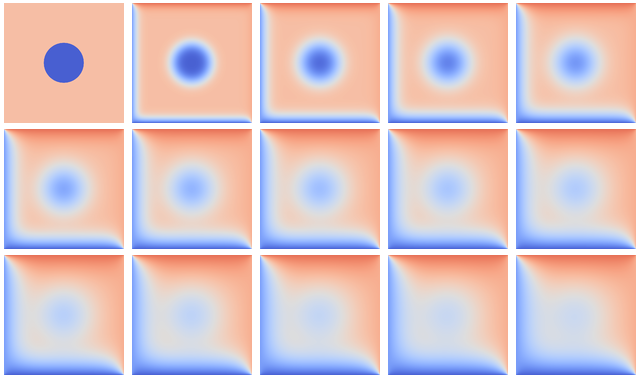
\includegraphics[width=0.7\textwidth]{fig_problem/heat_montage.png}
\caption{Over time, the temperature distribution in the rectangular area progresses from the initial state toward an end state where upper triangle is warm and lower is cold. The average temperature tends to (70+85+20+5)/4=45.}\label{fig:heat_montage}
\end{figure}


% ---------------------------------------------------------------------- %


\subsection{Technique: Stencil computation}


\par
Heat transfer in the system mentioned above is governed by the partial differential equation (PDE) describing local variation of the temperature field in time and space.
That is, the rate of change of the temperature field $u(x,y,t)$ over two spatial dimensions $x$ and $y$ and time $t$ (with rate coefficient $\alpha$) can be modelled via the equation
\begin{equation}
    \frac{\partial u}{\partial t} = \alpha \Big(\frac{\partial^2u}{\partial x^2} + \frac{\partial^2u}{\partial y^2}\Big) \,. \label{eq:heat_diffusion_pde}
\end{equation}

 
\par
The standard way to numerically solve the differential equations is to discretize them, $i.e.$, to consider only a set/grid of specific area points at specific moments in time.
That way, partial derivatives $\partial u$ are converted into differences between adjacent grid points $u^m(i,j)$, with $m$, $i$, $j$ denoting time and spatial grid points, respectively.
Temperature change in time at a certain point can now be computed from the values of neighboring points at earlier time; the same expression, called~\textbf{stencil} (shown in Fig.~\ref{fig:stencil}), is applied to every point on the grid.


\begin{figure}[!htbp]
\centering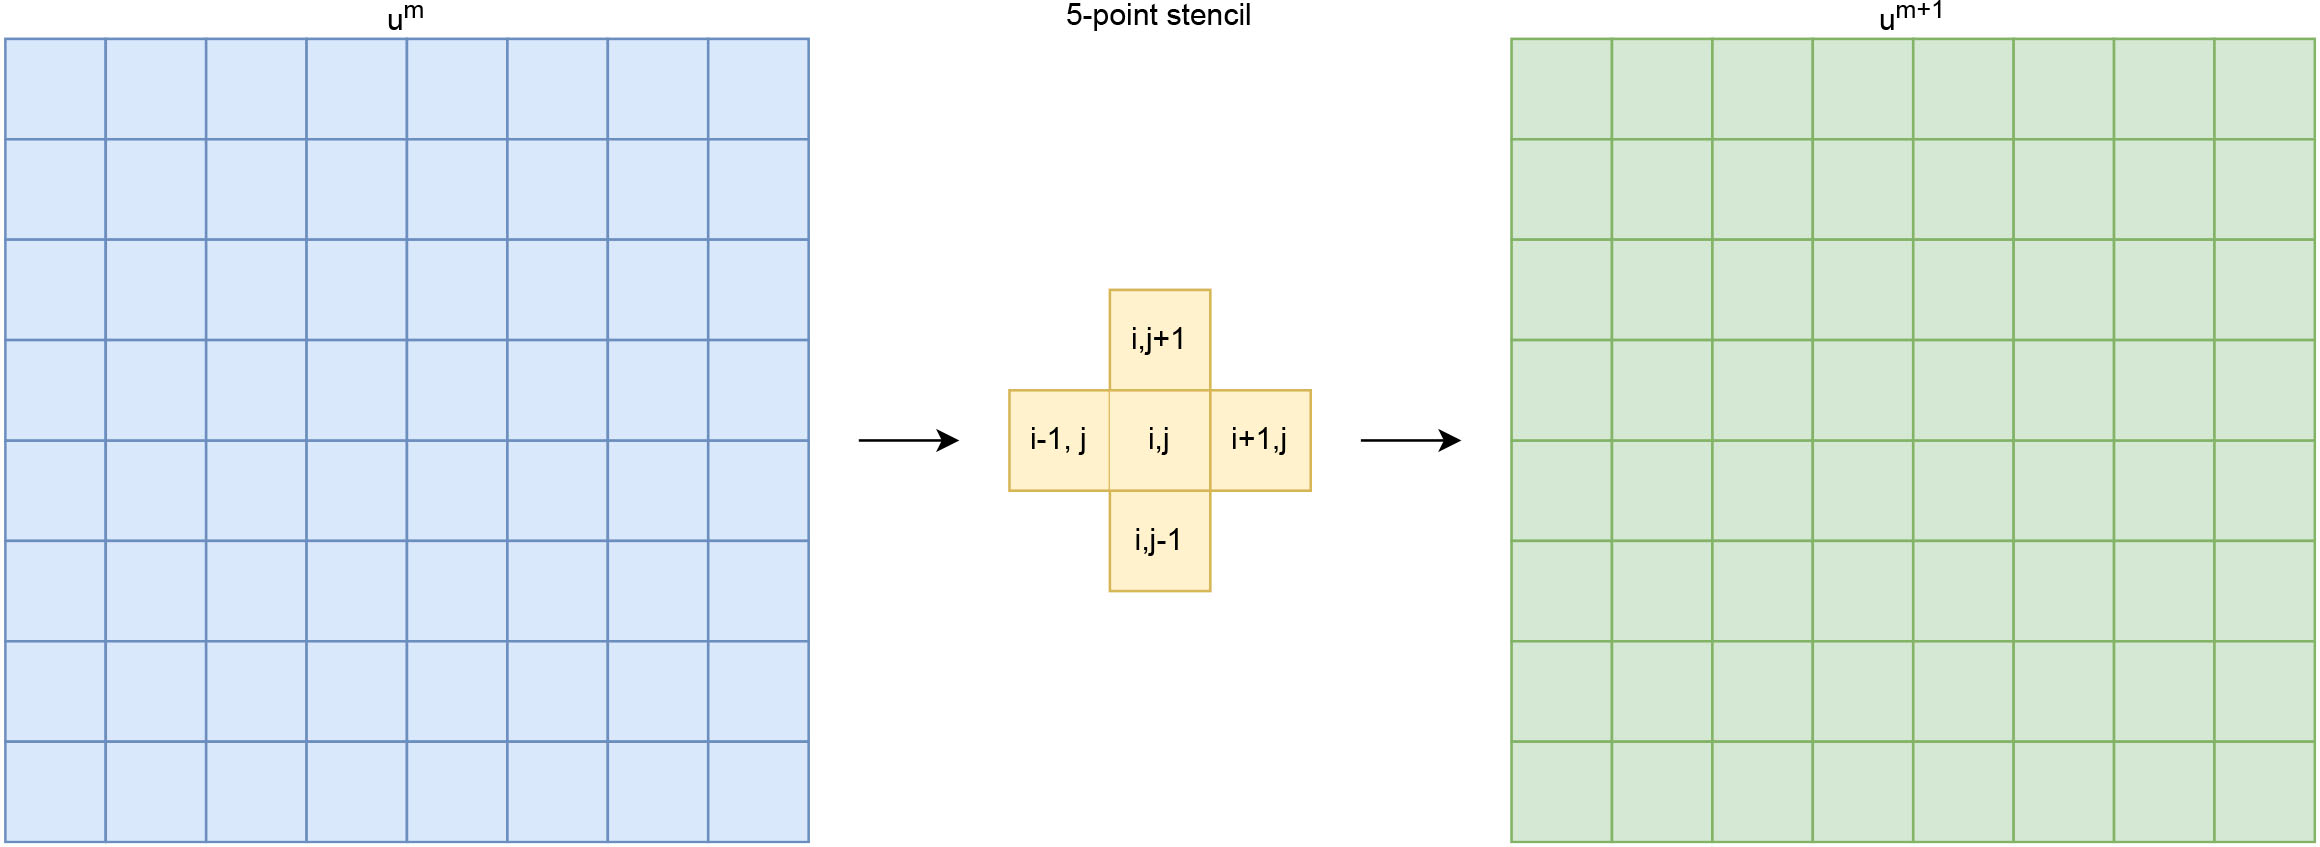
\includegraphics[width=0.8\textwidth]{fig_problem/stencil.jpg}
\caption{This simplified model uses an 8x8 grid of data in light blue in state $m$, each location of which has to be updated based on the indicated 5-point stencil in yellow to move to the next time point $m+1$.}\label{fig:stencil}
\end{figure}


\par
It should be mentioned that stencil computation is a common occurrence in solving numerical problems.
One obvious choice for stencil computations is the convolution operation.
Using the stencil convolution operation to solve the PDE for the heat diffusion, we will have several technical considerations.


\subsubsection{How fast and/or accurate can the solution be?}


\par
Spatial resolution of the temperature field is controlled by the number/density of the grid points.
As the full grid update is required to proceed from one time point to the next, stencil computation is the main target of parallelization (on CPU or GPU).
Moreover, in many cases the chosen time step cannot be arbitrarily large, otherwise the numerical differentiation will fail, and dense/accurate grids imply small time steps (see the equations below), which makes efficient spatial update even more important.


\par
One option for stencil expression and time-step limit is described below.
The differential equation shown in Eq.~\ref{eq:heat_diffusion_pde} can be discretized using different schemes.
For this example, the temperature values at each grid point $u^m(i,j)$ are updated from one time point ($m$) to the next ($m+1$), using the following expressions:
\begin{equation}
    u^{m+1}(i,j) = u^m(i,j) + \Delta t \alpha \nabla^2 u^m(i,j) \,,
\end{equation}
where 
\begin{equation}
    \nabla^2u = \frac{u(i-1,j)-2u(i,j)+u(i+1,j)}{(\Delta x)^2} + \frac{u(i,j-1)-2u(i,j)+u(i,j+1)}{(\Delta y)^2}\,,
\end{equation}
and $\Delta x$, $\Delta y$, $\Delta t$ are step sizes in space and time, respectively.
Time-update schemes also have a limit on the maximum allowed time step $\Delta t$.
For the current scheme, it is equal to
\begin{equation}
    \Delta t_{max} = \frac{(\Delta x)^2(\Delta y)^2}{2\alpha((\Delta x)^2+(\Delta y)^2)}\,.
\end{equation}


\subsubsection{What to do with area boundaries?}


\par
Naturally, stencil expression can’t be applied directly to the outermost grid points that have no outer neighbors. This can be solved by either changing the expression for those points or by adding an additional layer of grid that is used in computing update, but not updated itself – points of fixed temperature for the sides are being used in this example.


\subsubsection{How could the algorithm be optimized further?}


\par
In an earlier subsection~\ref{sec:memory_optimization}, importance of efficient memory access was already stressed.
In the following examples, each grid point (and its neighbors) is treated mostly independently; however, this also means that for 5-point stencil each value of the grid point may be read up to 5 times from memory (even if it’s the fast GPU memory).
By rearranging the order of mathematical operations, it may be possible to reuse these values in a more efficient way.


\par
Another point to note is that even if the solution is propagated in small time steps, not every step might actually be needed for output.
Once some local region of the field is updated, mathematically nothing prevents it from being updated for the second time step – even if the rest of the field is still being recalculated – as long as $t=m-1$ values for the region boundary are there when needed.
Of course, this is more complicated to implement and would only give benefits in certain cases.


% ---------------------------------------------------------------------- %


\subsection{Sequential and thread-parallel program in C++}


\par
Source files of the code examples presented for the rest of this section are available in the~\textbf{\textcolor{brown}{content/examples/stencil/}} subdirectory of this repository~\cite{gpu-programming-examples}.
You can use Git to download them to your home directory on the cluster.
It should be noted that do not forget to git pull for the latest updates if you already have the content from the first day of this workshop.
\lstinputlisting[language=bash, firstline=1, lastline=2, label={lst:13_heat_diffusion_stencil_path}, xleftmargin=0.05\textwidth, xrightmargin=0.05\textwidth]{code_examples/13_heat_diffusion_stencil_path.pbs}


\par
The general structure (main function), the default parameter values for the problem model, and the stencil update scheme of this program is shown in List~\ref{lst:13_heat_diffusion_stencil_cpu_main}, List~\ref{lst:13_heat_diffusion_stencil_cpu_params}, and List~\ref{lst:13_heat_diffusion_stencil_cpu_update}, respectively. 
If we assume the grid point values to be truly independent for a single time step, stencil application procedure may be straighforwardly written as a loop over the grid points, as shown in List~\ref{lst:13_heat_diffusion_stencil_cpu_update}.
The CPU-thread parallelism can then be enabled by a single OpenMP~\textbf{\textcolor{red}{\#pragma}} shown in the 26$^{th}$ line in List~\ref{lst:13_heat_diffusion_stencil_cpu_update}.


\lstinputlisting[language=c++, caption={The general structure (main function) for the head diffusion program in C++.}, label={lst:13_heat_diffusion_stencil_cpu_main}, xleftmargin=0.05\textwidth, xrightmargin=0.05\textwidth]{code_examples/13_heat_diffusion_stencil_cpu_main.cpp}


\lstinputlisting[language=c++, caption={The default parameter values for the head diffusion program in C++.}, label={lst:13_heat_diffusion_stencil_cpu_params}, xleftmargin=0.05\textwidth, xrightmargin=0.05\textwidth]{code_examples/13_heat_diffusion_stencil_cpu_params.cpp}
	

\lstinputlisting[language=c++, caption={The stencil update scheme for the head diffusion program in C++.}, label={lst:13_heat_diffusion_stencil_cpu_update}, xleftmargin=0.05\textwidth, xrightmargin=0.05\textwidth]{code_examples/13_heat_diffusion_stencil_cpu_update.cpp}


\subsubsection{Compiling executables and running OpenMP-CPU tests}


\par
Executable files for the OpenMP-enabled variants are provided together with the source code. However, if you’d like to compile them yourself, follow the instructions below:
\lstinputlisting[language=bash, firstline=1, lastline=6, label={13_heat_diffusion_stencil_cpu_openmp_lumi}, xleftmargin=0.05\textwidth, xrightmargin=0.05\textwidth]{code_examples/13_heat_diffusion_stencil_cpu_openmp_lumi.cpp}

Afterwards login into an interactive node and test the executables.
\lstinputlisting[language=bash, firstline=14, lastline=20, label={13_heat_diffusion_stencil_cpu_openmp_lumi}, xleftmargin=0.05\textwidth, xrightmargin=0.05\textwidth]{code_examples/13_heat_diffusion_stencil_cpu_openmp_lumi.cpp}

If everything works well, the output should look similar to this:
\lstinputlisting[language=bash, firstline=28, lastline=44, label={13_heat_diffusion_stencil_cpu_openmp_lumi}, xleftmargin=0.05\textwidth, xrightmargin=0.05\textwidth]{code_examples/13_heat_diffusion_stencil_cpu_openmp_lumi.cpp}


\par
Changing number of default OpenMP threads is somewhat tricky to do interactively, so OpenMP-CPU~\lq\lq scaling\rq\rq~tests are done via provided batch script (using~\textbf{\textcolor{brown}{squeue --me}} to make sure that there is no currently running interactive allocation.
\lstinputlisting[language=bash, firstline=52, lastline=58, label={13_heat_diffusion_stencil_cpu_openmp_lumi}, xleftmargin=0.05\textwidth, xrightmargin=0.05\textwidth]{code_examples/13_heat_diffusion_stencil_cpu_openmp_lumi.cpp}

The expected output is:
\lstinputlisting[language=bash, firstline=66, lastline=72, label={13_heat_diffusion_stencil_cpu_openmp_lumi}, xleftmargin=0.05\textwidth, xrightmargin=0.05\textwidth]{code_examples/13_heat_diffusion_stencil_cpu_openmp_lumi.cpp}


\subsubsection{Timing CPU parallelization}


\par
For later comparison, some benchmarks of the thread-parallel executable are provided below.

\begin{table}[!h]
\centering\caption{Run times of OpenMP-enabled executable in seconds.}\label{tbl:terminology}
\begin{tabular}{ |c|c|c| } 
\hline
\textbf{Job size} &  \textbf{1 CPU core} & \textbf{32 CPU cores} \\
\hline
S:2000 T:500 & 1.390 & 0.061 \\
S:2000 T:5000 & 13.900 & 0.550 \\
S:20000 T:50 & 15.200 & 12.340 \\
\hline
\end{tabular}
\end{table}


\par
A closer look at the left figure in Fig.~\ref{fig:heat_omp_step_gridside} reveals that the computation time scales very nicely with increasing time steps.
However, for larger grid sizes the parallelization becomes inefficient – as the individual chunks of the grid get too large to fit into CPU cache, threads become bound by the speed of RAM reads/writes, as shown at the right figure in Fig.~\ref{fig:heat_omp_step_gridside}.


\begin{figure}[!htbp]
\centering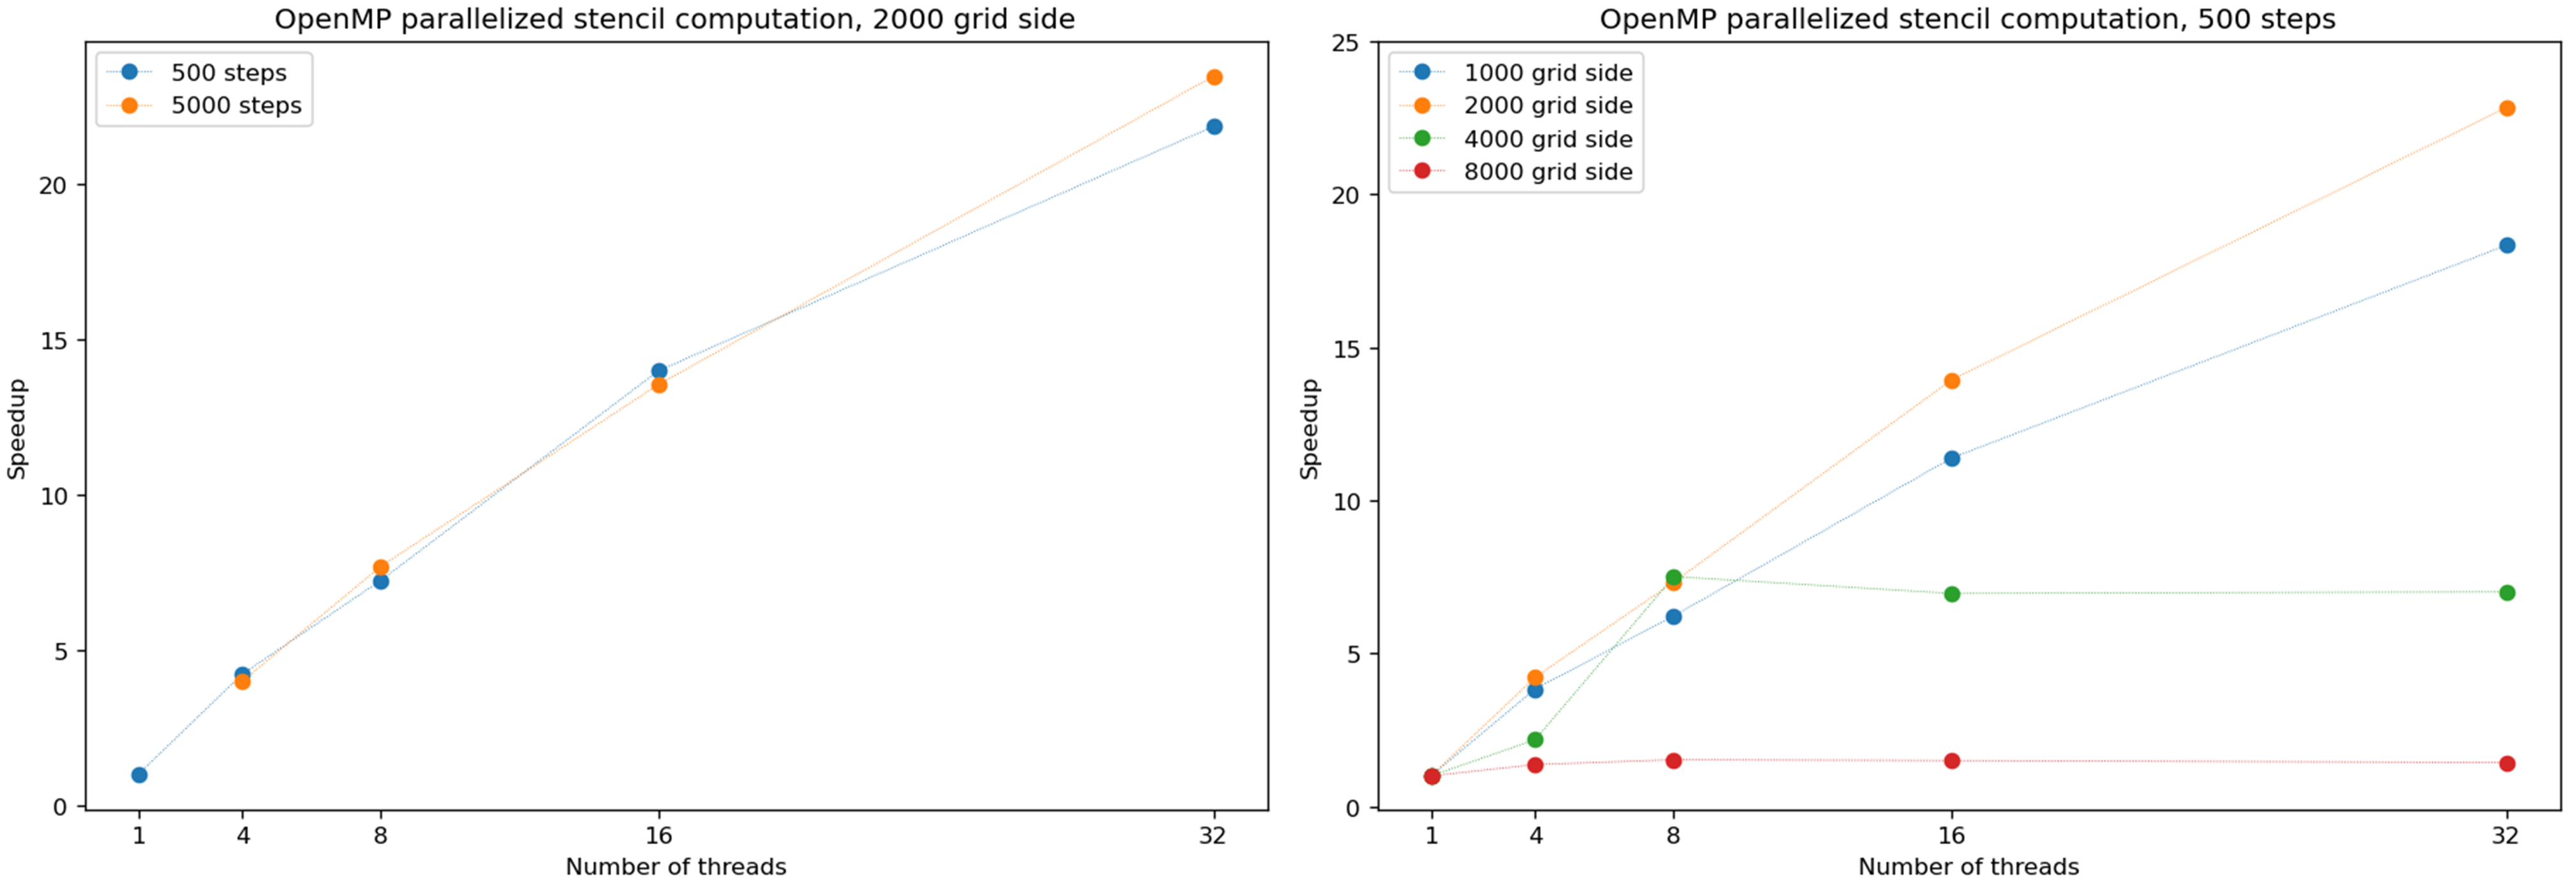
\includegraphics[width=0.9\textwidth]{fig_problem/heat_omp_step_gridside.png}
\caption{OpenMP parallelized stencil computations. Left for the computations with 2000 grid size at varied steps, and right for computations at 500 steps with varied number of grid side.}\label{fig:heat_omp_step_gridside}
\end{figure}


\par
A short summary of the heat flow computation scaling program.
\begin{itemize}
    \item The heat flow computation exhibits linear scaling behavior with respect to the number of time steps. Since each time-step update is sequential and involves a similar number of operations, the update time will be more or less constant.
    \item The stencil application (grid update) is expected to exhibit quadratic scaling character respect to the size of grid side. Since stencil application is independent for every grid point, the update time will be proportional to the number of points ($i.e.$, side * side).
    \item The GPU-accelerated computations are expected to suffer from the memory effect. GPU computations are indeed sensitive to memory access patterns and tend to resort to (GPU) memory quickly. However, the effect above arises because multiple active CPU threads start competing for access to RAM. In contrast,|\lq\lq over-subscribing\rq\rq~the GPU with large amount of threads executing the same kernel (stencil update on a grid point) tends to hide memory access latencies; increasing grid size might actually help to achieve this.
\end{itemize}


% ---------------------------------------------------------------------- %


\subsection{GPU parallelization}


\subsubsection{Porting sequential C++ code to naive GPU parallelization}


\par
Let’s apply several techniques presented in previous sections to make stencil update (List~\ref{lst:13_heat_diffusion_stencil_cpu_update}) GPU-parallel.
The OpenMP (or OpenACC) offloading requires to define a region to be executed in parallel as well as data that shall be copied over/used in GPU memory.
Similarly, the SYCL programming model offers convenient ways to define execution kernels, context to run them in (called queue) and simplified CPU-GPU transfer of needed data.
Changes of stencil update code shown in List~\ref{lst:13_heat_diffusion_stencil_cpu_update} for OpenMP and SYCL are shown in List~\ref{lst:13_heat_diffusion_stencil_gpu_openmp_naive} and List~\ref{lst:13_heat_diffusion_stencil_gpu_sycl_naive}, respectively.


\lstinputlisting[language=c++, caption={Changes of stencil update scheme shown in List~\ref{lst:13_heat_diffusion_stencil_cpu_update} in C++ for GPU programming using OpenMP.}, label={lst:13_heat_diffusion_stencil_gpu_openmp_naive}, xleftmargin=0.05\textwidth, xrightmargin=0.05\textwidth]{code_examples/13_heat_diffusion_stencil_gpu_openmp_naive.cpp}


\lstinputlisting[language=c++, caption={Changes of stencil update scheme shown in List~\ref{lst:13_heat_diffusion_stencil_cpu_update} in C++ for GPU programming using SYCL.}, label={lst:13_heat_diffusion_stencil_gpu_sycl_naive}, xleftmargin=0.05\textwidth, xrightmargin=0.05\textwidth]{code_examples/13_heat_diffusion_stencil_gpu_sycl_naive.cpp}


\subsubsection{Compiling SYCL executables}


\par
As SYCL is placed on top of ROCm/HIP (or CUDA) software stack, even running SYCL executables may require respective modules to be loaded.
On the LUMI-G nodes, it can be done as follows.
\lstinputlisting[language=bash, firstline=10, lastline=16, label={lst:13_heat_diffusion_stencil_path}, xleftmargin=0.05\textwidth, xrightmargin=0.05\textwidth]{code_examples/13_heat_diffusion_stencil_path.pbs}


\par
As described in previous sections, you can generate your own executables.
This time we will use the interactive allocation for GPU computing.
\lstinputlisting[language=bash, firstline=24, lastline=31, label={lst:13_heat_diffusion_stencil_path}, xleftmargin=0.05\textwidth, xrightmargin=0.05\textwidth]{code_examples/13_heat_diffusion_stencil_path.pbs}


\par
In the interactive allocation, run (using~\textbf{\textcolor{brown}{srun}}) provided or compiled executables~\textbf{\textcolor{brown}{base/stencil}},~\textbf{\textcolor{brown}{base/stencil\_off}} and~\textbf{\textcolor{brown}{sycl/stencil\_naive}}.
Try changing problem size parameters~\textbf{\textcolor{brown}{srun stencil\_naive 2000 2000 5000}} to see how computation time changes.


\subsubsection{Timing naive GPU parallelization}


\par
If you ran the code examples mentioned above for the heat diffusion program, you might already know that the GPU-\lq\lq ported\rq\rq~versions actually run slower than the single-CPU-core version.
In fact, the scaling behavior of all three variants is similar and expected, which is a good sign; only the~\lq\lq computation unit cost\rq\rq~is different.
You can compare benchmark summaries shown in Fig.~\ref{fig:heat_seq_openmp_sycl_naive}.


\begin{figure}[!htbp]
\centering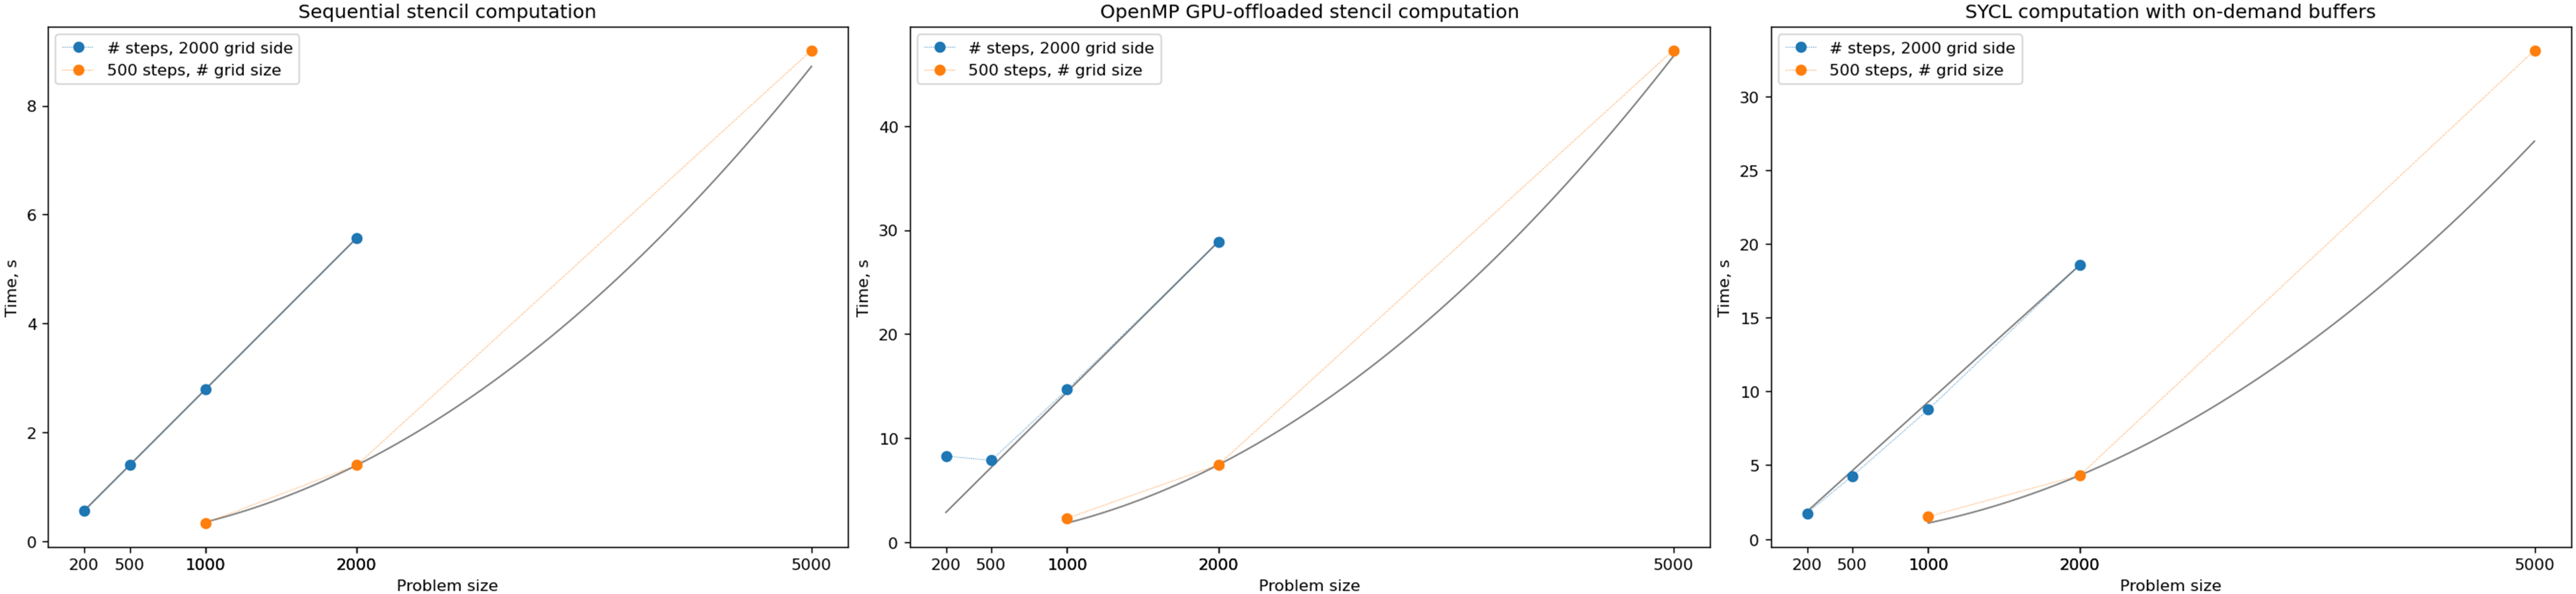
\includegraphics[width=0.9\textwidth]{fig_problem/heat_seq_openmp_sycl_naive.png}
\caption{Sequential and parallelized stencil computations. Left for the sequential stencil computations, middle for OpenMP GPU-offloaded stencil computations, and right for SYCL computations with on-demand buffers.}\label{fig:heat_seq_openmp_sycl_naive}
\end{figure}


\subsubsection{Data movement in GPU parallelization}


\par
Why the GPU-ported versions above seem to be grossly inefficient? At each step, we follow the right procedures for GPU progrmming: 1) re-allocate GPU memory; 2) copy data from CPU to GPU; 3) perform GPU computations; and 4) copy data back from GPU to CPU.
It was revealed that the steps for copying data from CPU to GPU and back are the most time consuming part during the code execution.
In fact the overhead can be reduced by taking following steps to minimize data transfers between host (CPU) and device (GPU) memory: 1) allocate GPU memory once at the start of the program; 2) only copy data from GPU to CPU when we need it; and 3) swap GPU buffers between timesteps, like we do with CPU buffers (OpenMP does this automatically).
As such, we can upgrade the stencil update code for OpenMP (List~\ref{lst:13_heat_diffusion_stencil_gpu_openmp_naive}) and SYCL (List~\ref{lst:13_heat_diffusion_stencil_gpu_sycl_naive}), and the obtained stencil update code are available at List~\ref{lst:13_heat_diffusion_stencil_gpu_openmp_naive_update} and List~\ref{lst:13_heat_diffusion_stencil_gpu_sycl_naive_update} for OpenMP and SYCL, respectively.
In addition, the main function for SYCL is provided in List~\ref{lst:13_heat_diffusion_stencil_gpu_sycl_naive_update_main}, and a naive version for Python is also provided in List~\ref{lst:13_heat_diffusion_stencil_gpu_python_naive} for a comparative purpose.


\lstinputlisting[language=c++, caption={Changes of stencil update scheme shown in List~\ref{lst:13_heat_diffusion_stencil_gpu_openmp_naive} for naive GPU parallelization using OpenMP.}, label={lst:13_heat_diffusion_stencil_gpu_openmp_naive_update}, xleftmargin=0.05\textwidth, xrightmargin=0.05\textwidth]{code_examples/13_heat_diffusion_stencil_gpu_openmp_naive_update.cpp}


\lstinputlisting[language=c++, caption={Changes of stencil update scheme shown in List~\ref{lst:13_heat_diffusion_stencil_gpu_sycl_naive} for naive GPU parallelization using SYCL.}, label={lst:13_heat_diffusion_stencil_gpu_sycl_naive_update}, xleftmargin=0.05\textwidth, xrightmargin=0.05\textwidth]{code_examples/13_heat_diffusion_stencil_gpu_sycl_naive_update.cpp}


\lstinputlisting[language=c++, caption={The main function for naive GPU parallelization using SYCL.}, label={lst:13_heat_diffusion_stencil_gpu_sycl_naive_update_main}, xleftmargin=0.05\textwidth, xrightmargin=0.05\textwidth]{code_examples/13_heat_diffusion_stencil_gpu_sycl_naive_update_main.cpp}


\lstinputlisting[language=python, caption={The main function for naive GPU parallelization using Python.}, label={lst:13_heat_diffusion_stencil_gpu_python_naive}, xleftmargin=0.05\textwidth, xrightmargin=0.05\textwidth]{code_examples/13_heat_diffusion_stencil_gpu_python_naive.py}


\subsubsection{Timing updated GPU parallelization}


\par
Again, we can run (using~\textbf{\textcolor{brown}{srun}}) the provided or compiled executables~\textbf{\textcolor{brown}{base/stencil\_data}} and~\textbf{\textcolor{brown}{sycl/stencil}} in the interactive allocation.
Try changing problem size parameters~\textbf{\textcolor{brown}{srun stencil 2000 2000 5000}} to see how computation time changes.


\par
Fig.~\ref{fig:heat_openmp_sycl_update} provides the output for these updated GPU computations.
Using GPU offloading with mapped GPU data, it is possible to achieve performance gains compared to the thread-parallel CPU version for larger grid sizes, due to the fact that the latter version becomes essentially RAM-bound, but the former does not.
In addition, because of the more explicit programming approach, SYCL GPU port is still 10 times faster than OpenMP offloaded version, comparable with thread-parallel CPU version running on all cores of a single node. Moreover, the performance scales perfectly with respect to both the grid size and the number of time steps (grid updates) computed.


\begin{figure}[htbp]
\centering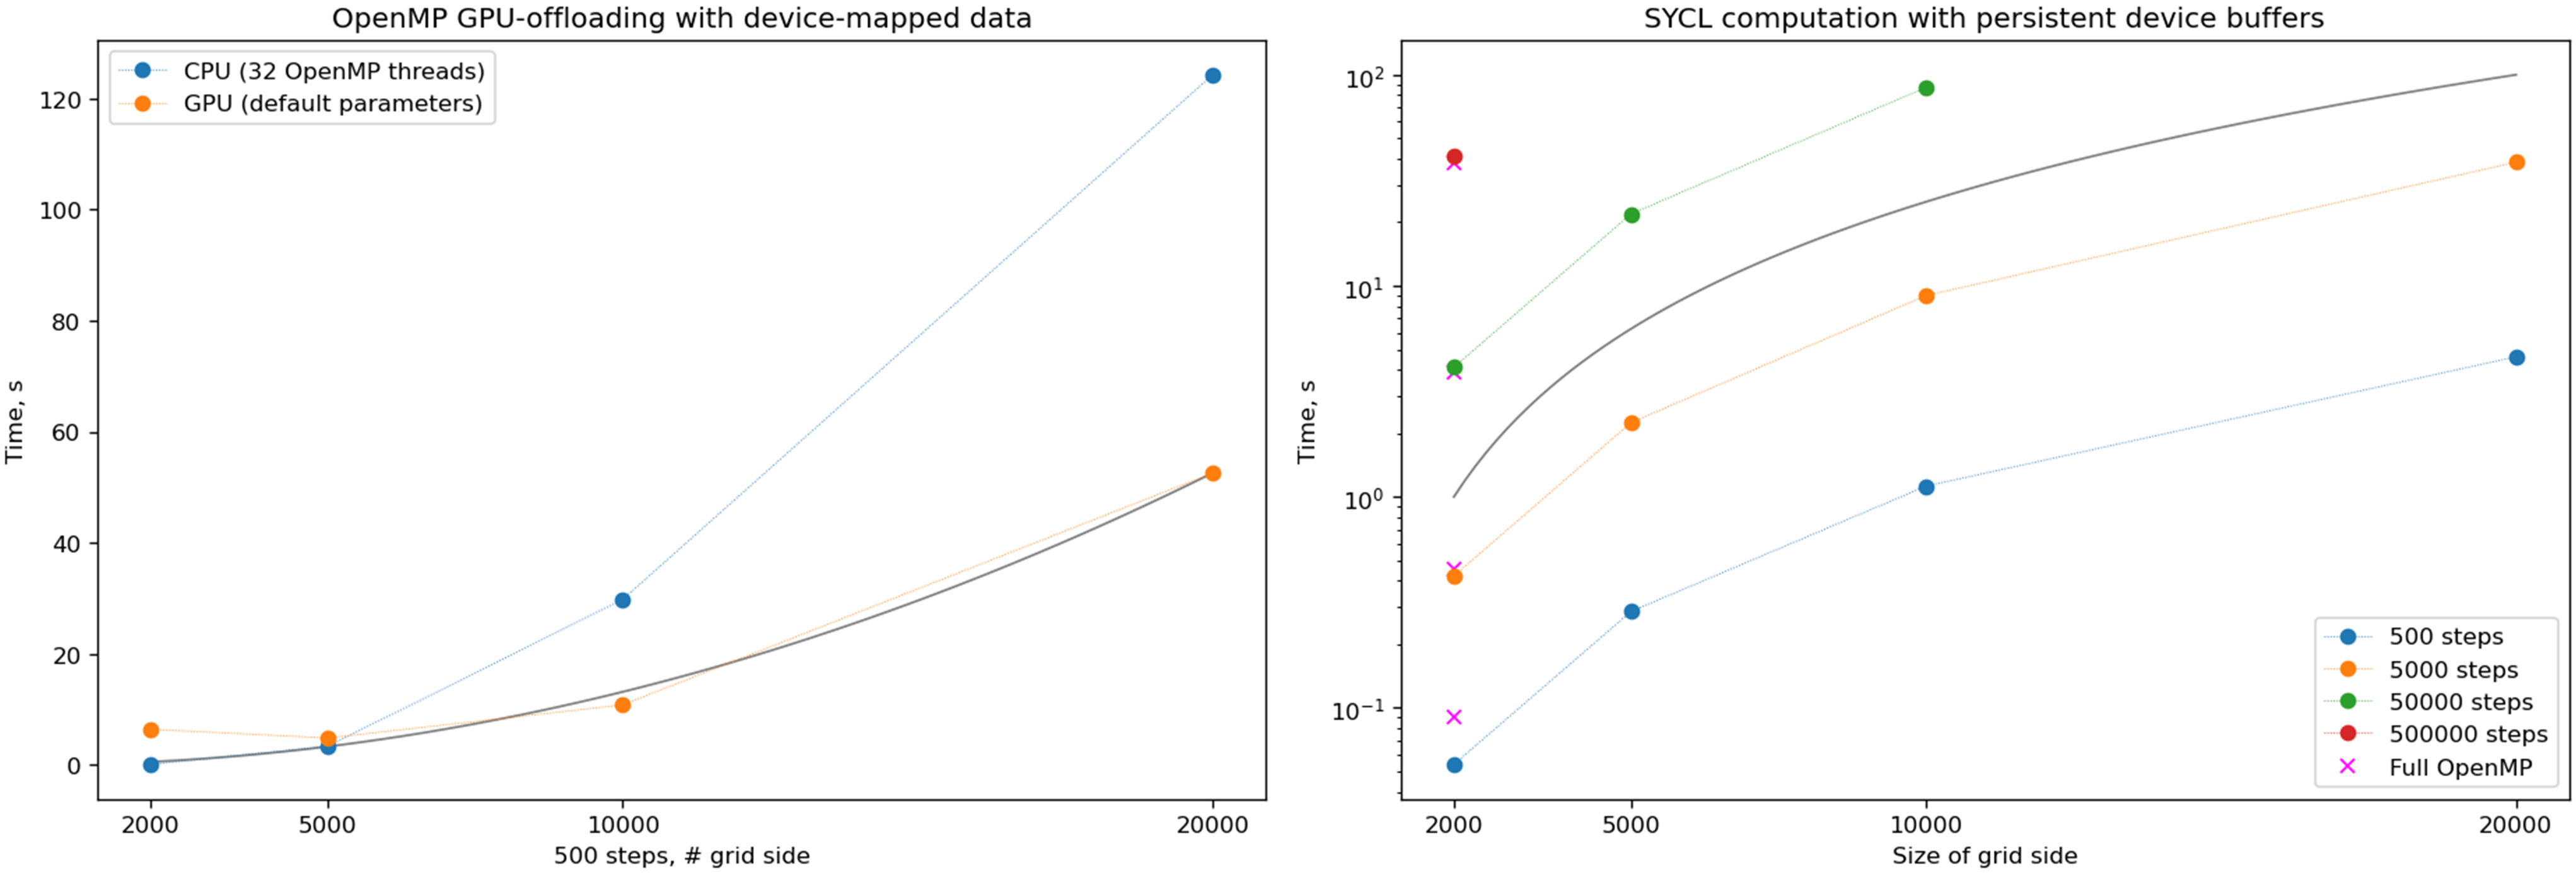
\includegraphics[width=0.9\textwidth]{fig_problem/heat_openmp_sycl_update.png}
\caption{Updated GPU parallelized stencil computations. Left for OpenMP GPU-offfloading with device-mapped data, and right fore SYCL GPU computation with persistent device buffers.}\label{fig:heat_openmp_sycl_update}
\end{figure}


% ---------------------------------------------------------------------- %


\subsection{Python: JIT and GPU acceleration}


\subsubsection{JIT acceleration in Python}


\par
As mentioned in previous subsections, the~\textbf{Numba} package allows developers to just-in-time (\textbf{JIT}) compile Python code to run fast on CPUs, but can also be used for JIT compiling for GPUs (although AMD GPU support is at the moment deprecated for Numba versions $>$ 0.53).
JIT seems to work well on loop-based, computationally heavy functions, so trying it out is a nice choice for initial source version.
The code examples for the stencil update scheme and the data generation function are provided in List~\ref{lst:13_heat_diffusion_stencil_gpu_python_jit_stencil_update} and List~\ref{lst:13_heat_diffusion_stencil_gpu_python_jit_data_generation}, respectively.


\lstinputlisting[language=python, caption={The stencil update scheme for Python GPU parallelization using JIT in Numba.}, label={lst:13_heat_diffusion_stencil_gpu_python_jit_stencil_update}, xleftmargin=0.05\textwidth, xrightmargin=0.05\textwidth]{code_examples/13_heat_diffusion_stencil_gpu_python_jit_stencil_update.py}


\lstinputlisting[language=python, caption={The data generation function for Python GPU parallelization using JIT in Numba.}, label={lst:13_heat_diffusion_stencil_gpu_python_jit_data_generation}, xleftmargin=0.05\textwidth, xrightmargin=0.05\textwidth]{code_examples/13_heat_diffusion_stencil_gpu_python_jit_data_generation.py}


\par
The alternative approach would be to rewrite stencil update code in NumPy style, exploiting loop vectorization.
You can try to run the provided Python examples using the Google Colab with instructions provided in the~\href{https://enccs.github.io/gpu-programming/0-setup/#running-on-google-colab}{Setup} on your local machine or LUMI node (non-GPU variants).
On LUMI, you can set up Python distribution as following:
\lstinputlisting[language=bash, firstline=40, lastline=47, label={lst:13_heat_diffusion_stencil_path}, xleftmargin=0.05\textwidth, xrightmargin=0.05\textwidth]{code_examples/13_heat_diffusion_stencil_path.pbs}


\par
A short summary of a typical Colab run is provided in Table~\ref{tbl:gpu_python_google_colab}. 
For later comparison, some benchmarks of the thread-parallel executable are provided in Table~\ref{tbl:gpu_python_google_colab}.


\begin{table}[!h]
\centering\caption{Run times of Numba JIT-enabled Python program in second.}\label{tbl:gpu_python_google_colab}
\begin{tabular}{ |c|c|c|c|c| } 
\hline
\textbf{Job size} & \textbf{JIT (LUMI)} & \textbf{JIT (Colab)} & \textbf{Job size} & \textbf{no JIT (Colab)} \\
\hline
S:2000 T:500 & 1.648 & 8.495 & S:200 T:50 & 5.318 \\
S:2000 T:200 & 0.787 & 3.524 & S:200 T:20 & 1.859 \\
S:1000 T:500 & 0.547 & 2.230 & S:100 T:50 & 1.156 \\
\hline
\end{tabular}
\end{table}


\par
Numba’s~\textbf{\textcolor{red}{@vectorize}} and~\textbf{\textcolor{red}{@guvectorize}} decorators offer an interface to create CPU- (or GPU-) accelerated Python functions without explicit implementation details.
However, such functions become increasingly complicated to write (and optimize by the compiler) with increasing complexity of the computations within.


\par
For NVIDIA GPUs, Numba also offers direct CUDA-based kernel programming, which can be the best choice for those already familiar with CUDA.
An example for stencil update written in Numba CUDA is shown in List~\ref{lst:13_heat_diffusion_stencil_gpu_python_naive}.
In this case, the data transfer functions~\textbf{\textcolor{red}{devdata = cuda.to\_device(data)}} and~\textbf{\textcolor{red}{devdata.copy\_to\_host(data)}} shown in the~\textbf{\textcolor{brown}{main\_cuda.py}} are already provided by the Numba package.


\subsubsection{CUDA acceleration in Python}


\par
Using the Google Colab (or your own machine), run provided Numba-CUDA Python program.
Try to change problem size parameters and rerun the computations:
\begin{itemize}
    \item \textbf{\textcolor{brown}{args.rows, args.cols, args.nsteps = 2000, 2000, 5000}} for notebooks.
    \item \textbf{\textcolor{brown}{srun python3 main.py 2000 2000 5000}} for command line.
\end{itemize}


\par
The obtained numbers from Google Colab are listed in Table~\ref{tbl:gpu_python_google_colab_numba}.


\begin{table}[!h]
\centering\caption{Run times of Numba CUDA Python program in second.}\label{tbl:gpu_python_google_colab_numba}
\begin{tabular}{ |c|c|c|c| } 
\hline
\textbf{Job size} & \textbf{JIT (LUMI)} & \textbf{JIT (Colab)} & \textbf{CUDA (Colab)} \\
\hline
S:2000 T:500 & 1.648 & 8.495 & 1.079 \\
S:2000 T:2000 & 6.133 & 36.61 & 3.931 \\
S:5000 T:500 & 9.478 & 57.19 & 6.448 \\
\hline
\end{tabular}
\end{table}


% ---------------------------------------------------------------------- %


\subsection{Julia acceleration}


\subsubsection{Julia code for CPU}


\par
A Julia version of the stencil example discussed above can be found below.
A simplified version of the HeatEquation module is provided at the~\href{https://github.com/ENCCS/HeatEquation.jl}{ENCCS repository}.
The source files are also available in the~\textbf{\textcolor{brown}{content/examples/stencil/julia}} subdirectory of this repository~\cite{gpu-programming-examples}.


\par
To run the example on the LUMI CPU partition, you should the following commands:
\lstinputlisting[language=bash, firstline=57, lastline=69, label={lst:13_heat_diffusion_stencil_path}, xleftmargin=0.05\textwidth, xrightmargin=0.05\textwidth]{code_examples/13_heat_diffusion_stencil_path.pbs}


\par
To run the example on the LUMI GPU partition, use instead the command below:
\lstinputlisting[language=bash, firstline=78, lastline=78, label={lst:13_heat_diffusion_stencil_path}, xleftmargin=0.05\textwidth, xrightmargin=0.05\textwidth]{code_examples/13_heat_diffusion_stencil_path.pbs}


\par
The code examples consisting of~\textbf{\textcolor{brown}{main.jl}},~\textbf{\textcolor{brown}{core.jl}},~\textbf{\textcolor{brown}{heat.jl}}, and~\textbf{\textcolor{brown}{project.toml}} are provided in List~\ref{lst:13_heat_diffusion_julia_main}, List~\ref{lst:13_heat_diffusion_julia_core}, List~\ref{lst:13_heat_diffusion_julia_heat}, and List~\ref{lst:13_heat_diffusion_julia_proj}, respectively.


\lstinputlisting[language=c++, caption={The~\textbf{\textcolor{brown}{main.jl}} file for the heat diffusion program in Julia.}, label={lst:13_heat_diffusion_julia_main}, xleftmargin=0.05\textwidth, xrightmargin=0.05\textwidth]{code_examples/13_heat_diffusion_julia_main.jl}


\lstinputlisting[language=c++, caption={The~\textbf{\textcolor{brown}{core.jl}} file for the heat diffusion program in Julia.}, label={lst:13_heat_diffusion_julia_core}, xleftmargin=0.05\textwidth, xrightmargin=0.05\textwidth]{code_examples/13_heat_diffusion_julia_core.jl}


\lstinputlisting[language=c++, caption={The~\textbf{\textcolor{brown}{heat.jl}} file for the heat diffusion program in Julia.}, label={lst:13_heat_diffusion_julia_heat}, xleftmargin=0.05\textwidth, xrightmargin=0.05\textwidth]{code_examples/13_heat_diffusion_julia_heat.jl}


\lstinputlisting[language=c++, caption={The~\textbf{\textcolor{brown}{project.toml}} file for the heat diffusion program in Julia.}, label={lst:13_heat_diffusion_julia_proj}, xleftmargin=0.05\textwidth, xrightmargin=0.05\textwidth]{code_examples/13_heat_diffusion_julia_project.toml}


\par
Note that the~\textbf{\textcolor{brown}{plots.jl}} dependency is commented out in~\textbf{\textcolor{brown}{main.jl}} (the 1$^{st}$, 35-36, and 41-42 lines in List~\ref{lst:13_heat_diffusion_julia_main}) and~\textbf{\textcolor{brown}{project.toml}} (the 3$^{rd}$ line in List~\ref{lst:13_heat_diffusion_julia_proj}) files.
This saves ~2 minute precompilation time when you first instantiate the Julia environment.
To generate plots, just uncomment the commented~\textbf{\textcolor{brown}{plots.jl}} dependency in the~\textbf{\textcolor{brown}{project.toml}} file (List~\ref{lst:13_heat_diffusion_julia_proj}), instantiate again, and import and use~\textbf{\textcolor{brown}{Plots}} in the~\textbf{\textcolor{brown}{main.jl}} file (List~\ref{lst:13_heat_diffusion_julia_main}).


\subsubsection{Julia port to GPU}


\par
Carefully inspect all Julia source files and consider the following questions:
\begin{itemize}
    \item Which functions should be ported to run on GPU?
    \item Look at the $initialize!()$ function and how it uses the $arraytype$ argument. This could be done more compactly and elegantly, but this solution solves scalar indexing errors. What are scalar indexing errors?
    \item Try to start sketching GPU-ported versions of the key functions.
    \item When you have a version running on a GPU (your own or the solution provided below), try benchmarking it by adding~\textbf{\textcolor{red}{@btime}} in front of $simulate!()$ in the~\textbf{\textcolor{brown}{main.jl}} file. Benchmark also the CPU version, and compare the obtained computational results.
\end{itemize}


\par
Some simple hints are provided below:
\begin{itemize}
    \item create a new function $evolve\_gpu!()$ which contains the GPU kernelized version of $evolve!()$;
    \item in the loop over timesteps in $simulate!()$, you will need a conditional like $if typeof(curr.data) <: ROCArray$ to call your GPU-ported functional;
    \item you cannot pass the struct $Field$ to the kernel. You will instead need to directly pass the array $Field.data$. This also necessitates passing in other variables like $curr.dx^2$, $etc$.
\end{itemize}


\par
More hints to upgrade the code for GPU acceleration using Julia are listed here.
\begin{itemize}
    \item since the data is two-dimensional, you’ll need $i = (blockIdx().x - 1) * blockDim().x + threadIdx().x$ and $j = (blockIdx().y - 1) * blockDim().y + threadIdx().y$;
    \item not to overindex the 2D array, you can use a conditional like $if~i>1~\&\&~j > 1~\&\&~i < nx+2~\&\&~j < ny+2$;
    \item when calling the kernel, you can set the number of threads and blocks like $xthreads = ythreads = 16$ and $xblocks, yblocks = cld(curr.nx, xthreads), cld(curr.ny, ythreads)$.
    \item call it with the command, $e.g.$, $@roc~threads=$ $(xthreads, ythreads) blocks=$ $(xblocks, yblocks)$ $evolve\_rocm!(curr.data,prev.data,curr.dx^2,curr.dy^2,nx,ny,a,dt)$.
\end{itemize}


\par
The solution for GPU acceleration using Julia are described below, and the code examples of~\textbf{\textcolor{brown}{main\_gpu.jl}} and~\textbf{\textcolor{brown}{core\_gpu.jl}} are provided in List~\ref{lst:13_heat_diffusion_julia_main_gpu} and List~\ref{lst:13_heat_diffusion_julia_core_gpu}, respectively.
\begin{itemize}
    \item The $evolve!()$ and $simulate!()$ functions need to be ported. The~\textbf{\textcolor{brown}{main.jl}} (List~\ref{lst:13_heat_diffusion_julia_main}) file also needs to be updated to work with GPU arrays.
    \item \lq\lq Scalar indexing\rq\rq~is the place where you iterate over a GPU array, which would be excruciatingly slow and is indeed only allowed in interactive REPL sessions. Without the if-statements in the $initialize!()$ function, the $generate\_field!()$ method would be doing disallowed scalar indexing if you were running on a GPU.
    \item The GPU-ported version is found below. Try it out on both CPU and GPU and observe the speedup. Play around with array size to see if the speedup is affected. You can also play around with the $xthreads$ and $ythreads$ variables to see if it changes anything.
\end{itemize}


\lstinputlisting[language=c++, caption={The~\textbf{\textcolor{brown}{main\_gpu.jl}} file for GPU acceleration of the heat diffusion program in Julia.}, label={lst:13_heat_diffusion_julia_main_gpu}, xleftmargin=0.05\textwidth, xrightmargin=0.05\textwidth]{code_examples/13_heat_diffusion_julia_main_gpu.jl}


\lstinputlisting[language=c++, caption={The~\textbf{\textcolor{brown}{core\_gpu.jl}} file for GPU acceleration of the heat diffusion program in Julia.}, label={lst:13_heat_diffusion_julia_core_gpu}, xleftmargin=0.05\textwidth, xrightmargin=0.05\textwidth]{code_examples/13_heat_diffusion_julia_core_gpu.jl}


\par
In summary, this section leans heavily on source code and material created for several other computing workshops by~\href{https://enccs.se/}{ENCCS} and~\href{https://www.csc.fi/en/home}{CSC} and adapted for the purposes of this lesson.
If you want to know more about specific programming models/framework, definitely check the reading materials below.
\begin{itemize}
    \item~\href{https://enccs.github.io/openmp-gpu/}{OpenMP for GPU offloading}
    \item~\href{https://enccs.github.io/sycl-workshop/}{Heterogeneous programming with SYCL}
    \item~\href{https://github.com/cschpc/heat-equation/}{Educational implementation of heat flow example} (incl. MPI-aware CUDA)
\end{itemize}



% -------------------------------------------------------------------- %
\clearpage
\section{List of Abbreviations}

%\chaptermark{List of Abbreviationsyyy}

\begin{abbrv}
\item[API]                   Application Programming Interface
\item[BPG]                   Best Practice Guide
\item[CHCAA]                 Center for Humanities Computing Aarhus
\item[CPU]                   Central Processing Unit
\item[CU]                    Computing Unit
\item[CUDA]                  Compute Unified Device Architecture
\item[DAG]                   Directed Acyclic Graph
\item[ERI]                   Electron Repulsion Integrals
\item[EU]                    Execution Unit
\item[FPGAs]                 Field Programmable Gate Arrays
\item[GPC]                   GPU Processing Clusters
\item[GPU]                   Graphics Processing Unit
\item[HIP]                   Heterogeneous-computing Interface for Portability
\item[HPC]                   High Performance Computing
\item[IMC]                   Interacting Minds Centre
\item[JIT]                   Just-in-Time
\item[LLVM]                  Low Level Virtual Machine)
\item[MCMC]                  Markov Chain Monte Carlo
\item[MIMD]                  Multiple Instruction Multiple Data
\item[MPI]                   Message Passing Interface
\item[NLP]                   Natural Language Processing
\item[OpenACC]               Open Accelerator
\item[OpenCL]                Open Computing Language
\item[OpenMP]                Open Multi-Processing
\item[PDE]                   Partial Differential Equation
\item[RDMA]                  Remote Direct Memory Access
\item[ROCm]                  Radeon Open Compute
\item[SDK]                   Software Development Kit
\item[SIMD]                  Single Instruction Multiple Data
\item[SIMT]                  Single Instruction Multiple Threads
\item[SMP]                   Streaming Multi-Processor
\item[SP]                    Streaming Processors
\item[SVM]                   Shared Virtual Memory
\item[USM]                   Unified Shared Memory
\item[VASP]                  Vienna Ab initio Simulation Package
\end{abbrv}


% -------------------------------------------------------------------- %
\clearpage
\section*{Further Documentation}
\bibliography{gpu_programming_bpg}



\end{document}
%{\centering{\textcolor{red}{\bf{\Huge WYL @ \today~\currenttime}}}}\\
